\documentclass[sigconf, nonacm]{acmart}

%% The following content must be adapted for the final version
% paper-specific
\newcommand\vldbdoi{XX.XX/XXX.XX}
\newcommand\vldbpages{XXX-XXX}
% issue-specific
\newcommand\vldbvolume{14}
\newcommand\vldbissue{1}
\newcommand\vldbyear{2020}
% should be fine as it is
\newcommand\vldbauthors{\authors}
\newcommand\vldbtitle{\shorttitle} 
% leave empty if no availability url should be set
\newcommand\vldbavailabilityurl{URL_TO_YOUR_ARTIFACTS}
% whether page numbers should be shown or not, use 'plain' for review versions, 'empty' for camera ready
\newcommand\vldbpagestyle{plain}


\usepackage[utf8]{inputenc}
\usepackage{times}
\usepackage{graphicx}
\usepackage{xcolor}
\usepackage{hyperref}
\usepackage{paralist}
\usepackage{listings}
\usepackage[inline]{enumitem}

\usepackage{microtype} % character spacing

\usepackage{booktabs} %added for tables (Andre)
\usepackage{algorithm}
\usepackage[noend]{algpseudocode}
\usepackage{svg}

\usepackage{xparse}
\makeatletter
\NewDocumentCommand{\LeftComment}{s m}{%
	\Statex \IfBooleanF{#1}{\hspace*{\ALG@thistlm}}\(\triangleright\) #2}
\makeatother

\definecolor{dkgreen}{rgb}{0,0.6,0}
\definecolor{gray}{rgb}{0.5,0.5,0.5}
\definecolor{mauve}{rgb}{0.58,0,0.82}
\lstset{language=SQL,
  basicstyle={\small\ttfamily},
  deletekeywords={key}, %not working
  belowskip=3mm,
  breakatwhitespace=true,
  breaklines=true,
  classoffset=0,
  columns=flexible,
  commentstyle=\color{dkgreen},
  framexleftmargin=0.25em,
  frameshape={}{}{}{},
  %frameshape={}{yy}{}{}, %To remove to vertical lines on left, set `frameshape={}{}{}{}`
  keywordstyle=\color{blue},
  numbers=none, %If you want line numbers, set `numbers=left`
  numberstyle=\tiny\color{gray},
  showstringspaces=false,
  stringstyle=\color{mauve},
  tabsize=3,
  xleftmargin =0em
}

\newcommand{\qcr}[1]{{\fontfamily{qcr}\selectfont #1}}
\newcommand{\code}[1]{\textsf{\small{#1}}}


\usepackage{balance}  % for  \balance command ON LAST PAGE  (only there!)

\usepackage{subcaption}
\graphicspath{{./images/}}

%Makes compact lists a little bit less compact
\setlength{\pltopsep}{0.3em}
\setlength{\plitemsep}{0.1em}

%\newcommand{\grumbler}[2]{{\color{red}{\bf #1:} #2}}
%\renewcommand{\grumbler}[2]{}
%\newcommand{\andre}[1]{\grumbler{andre}{#1}}
%\newcommand{\nuno}[1]{\grumbler{nuno}{#1}}
%\newcommand{\carla}[1]{\grumbler{carla}{#1}}

\newcommand{\outline}[1]{}
%\newcommand{\outline}[1]{\grumbler{outline}{#1}}

\newcommand{\emphvspace}{0.5\baselineskip}
%Single line
\newcommand{\lineemph}[1]{\vspace{\emphvspace}\hspace{2em}\emph{#1}\vspace{\emphvspace}}
%Multi line
\newcommand{\firstblockemph}[1]{\vspace{\emphvspace}\hspace{2em}\emph{#1}}
\newcommand{\middleblockemph}[1]{\hspace{2em}\emph{#1}}
\newcommand{\lastblockemph}[1]{\hspace{2em}\emph{#1}\vspace{\emphvspace}}
\newcommand{\emphfunction}[2]{\emph{#1}($#2$)}

\newtheorem{theorem}{Theorem}

\lstset{columns=fullflexible,
        mathescape=true,
        literate=
               {=}{$\leftarrow{}$}{1}
               {==}{$={}$}{1},
        morekeywords={fun}
        }

\definecolor{red}{RGB}{200,0,0}
\definecolor{green}{RGB}{0,200,0}
\definecolor{blue}{RGB}{0,0,200}
\usepackage{ifthen}
\newboolean{showcomments}
\setboolean{showcomments}{true} %
\ifthenelse{\boolean{showcomments}}
{\newcommand{\nbnote}[3]{
  %
  \fcolorbox{gray}{yellow}{\bfseries\sffamily\scriptsize#1}
  {\color{#2} \sffamily\small$\blacktriangleright$\textit{#3}$\blacktriangleleft$}
%
  %
  }
}
{\newcommand{\nbnote}[3]{}
 \newcommand{\version}{}
}
\newcommand{\andre}[1]{\nbnote{Andre}{blue}{#1}}
\newcommand{\carla}[1]{\nbnote{Carla}{green}{#1}}
\newcommand{\nuno}[1]{\nbnote{Nuno}{red}{#1}}


\begin{document}

\title{Global Views on Partially Geo-Replicated Data}

%%
%% The "author" command and its associated commands are used to define the authors and their affiliations.

\author{André Rijo, Carla Ferreira, Nuno Preguiça}
\affiliation{
\institution{NOVA LINCS, FCT, Universidade NOVA de Lisboa}
\country{Portugal}
}
%\email{a.rijo@campus.fct.unl.pt}
%\author{Carla Ferreira}
%\affiliation{NOVA LINCS, FCT, Universidade NOVA de Lisboa}
%\email{carla.ferreira@fct.unl.pt}
%\author{Nuno Preguiça}
%\affiliation{NOVA LINCS, FCT, Universidade NOVA de Lisboa}
%\email{nuno.preguica@fct.unl.pt}





\begin{abstract}

Many existing web services at a global scale have strict latency, availability, and fault tolerance requirements.
To address these requirements,  services are often deployed in data centers distributed 
across the globe, with users accessing the closest data center.
As the number of servers increases, so does the replication cost, which makes partial replication an attractive approach.
However, some queries may require data not replicated in every server (e.g. in an e-commerce system, the best-selling products across the globe).

In this paper, we present PotionDB, a novel geo-distributed key-value store that provides partial replication.
We present a replication scheme that allows data to be partially replicated, yet still, answer queries relative to global data efficiently.
We leverage existing partial and non-uniform replication algorithms to provide materialized views of data that may be split across multiple servers.
With these views, a client can obtain global information by querying a single server.
Our evaluation shows that queries concerning global data can be completed in less than one millisecond while maintaining high throughput, despite the extra operations required to keep views up-to-date. 

\end{abstract}


\maketitle


%%% do not modify the following VLDB block %%
%%% VLDB block start %%%
\pagestyle{\vldbpagestyle}
\begingroup\small\noindent\raggedright\textbf{PVLDB Reference Format:}\\
\vldbauthors. \vldbtitle. PVLDB, \vldbvolume(\vldbissue): \vldbpages, \vldbyear.\\
\href{https://doi.org/\vldbdoi}{doi:\vldbdoi}
\endgroup
\begingroup
\renewcommand\thefootnote{}\footnote{\noindent
This work is licensed under the Creative Commons BY-NC-ND 4.0 International License. Visit \url{https://creativecommons.org/licenses/by-nc-nd/4.0/} to view a copy of this license. For any use beyond those covered by this license, obtain permission by emailing \href{mailto:info@vldb.org}{info@vldb.org}. Copyright is held by the owner/author(s). Publication rights licensed to the VLDB Endowment. \\
\raggedright Proceedings of the VLDB Endowment, Vol. \vldbvolume, No. \vldbissue\ %
ISSN 2150-8097. \\
\href{https://doi.org/\vldbdoi}{doi:\vldbdoi} \\
}\addtocounter{footnote}{-1}\endgroup
%%% VLDB block end %%%

%%% do not modify the following VLDB block %%
%%% VLDB block start %%%
\ifdefempty{\vldbavailabilityurl}{}{
\vspace{.3cm}
\begingroup\small\noindent\raggedright\textbf{PVLDB Artifact Availability:}\\
The source code, data, and/or other artifacts have been made available at \url{\vldbavailabilityurl}.
\endgroup
}
%%% VLDB block end %%%

\section{Introduction}
\label{sec:introduction}

%	\item Num. DC a aumentar

The increasing reliance on web services in many domains of activity, from e-commerce to business applications
and entertainment, leads to stringent requirements regarding latency, availability,
and fault tolerance~\cite{Schurman2009latency,gomez}.
To address these requirements, cloud platforms have been adding new data centers at different geographic 
locations. By allowing users to access a service by contacting the closest data center, a global service can
provide low latency to users spread across the globe. The increasing number of data centers also contributes
for proving high availability and fault tolerance, by allowing a user to access the service by accessing any
available data center.

% serviços necessitam de data
% Replicar totalmente tem problemas

The database is a key component of any web service, storing the service's data. For supporting global
services running at multiple geographic locations, it is necessary to rely on a geo-replicated database~\cite{dynamo},
which maintains replicas of the data at the data centers where the service is running.
A number of geo-replicated databases have been proposed, providing different consistency semantics.
Databases that provide strong consistency \cite{spanner,cockroachdb,mdcc} intend to give  the illusion that 
a single replica exists, requiring coordination among
multiple replicas for executing (update) operations. This leads to high latency and may compromise 
availability in the presence of network partitions.
Databases that provide weak consistency \cite{eventual,dynamo,cops} allow any replica to process a
client request, leading to lower latency and high availability. As a consequence, these databases expose
temporary state divergence to clients, making it more difficult to program a system. 

Either case, geo-replicated databases usually rely on a full replication model, where each data 
center replicates the full database, with data being sharded across multiple partitions in each data 
center. 
As both the data managed by these systems increases in size and the number of data centers increases,
this approach leads to a number of problems.
First, storing all data in all data centers imposes a large overhead in terms of storage. 
Furthermore, storing some data in all data centers may be unnecessary, as data is only needed at some
geographic locations.
Second, increasing the number of data centers makes the replication process more complex and costly, 
as each update needs to be propagated to all other data centers.

For addressing these problems, partial replication is an attractive approach, with each data center
replicating only a subset of the data.
A number of works have been addressing the challenges of 
partial replication, for example by proposing algorithms to manage partially replicated data \cite{spanner,saturn,sipre, practi} and to decide which data is replicated in which replica \cite{slog, sipre}.

In this paper we address the problem of querying data in a weakly consistent partially geo-replicated database, 
focusing on recurrent queries for which the application could use a (materialized) view.
For example, consider an e-commerce system with users from multiple geographic locations.
In this case, the data pertaining users of a given location does not need to be replicated in all data centers
(but only in a few for fault tolerance). The same applies to other information, such as data on orders and 
warehouses.
Other data, such as information on products would be replicated in the regions where the product
is available for sale.  
Under this data placement, obtaining the list of best seller products is challenging, as it requires
accessing data that is located at multiple data centers.

Several possible solutions exist for this problem. 
First, it is possible to have a data center that replicates all data, and forward these queries to such data center.
Doing this imposes a latency penalty and requires a data center to host all data and execute all queries of this type. %Andre: also refer that this data center would be the bottleneck of the system?
Second, it is possible to execute the query by accessing multiple locations, by using, for example, 
a distributed processing system with support for geo-partitioned data \cite{kloudas2015pixida,jetstream}.
This approach requires running an additional external service and poses challenges for the consistency of the results returned and the data observed by users.
%, mostly when adopting weak consistency models (a local update that should
%be reflected in the result of the query may not be returned, as the update might have not been read by the 
%external service that accessed a different replica).

We propose a different approach: to maintain materialized views, as commonly available in relational databases.
Implementing such feature efficiently in a partially geo-replicated database requires 
addressing two main challenges. 
First, it is necessary to guarantee consistency between the base data available in a replica and the 
relevant materialized views. To achieve this, we designed both a transaction execution and a replication mechanism where updates 
to the base data and views are made visible atomically in each replica.

Second, it is necessary to efficiently support views with limits, used for example to support \emph{topK} 
queries. \carla{Later on top-k is defined as topK.}
To achieve this, we build on the concept of non-uniform replication \cite{Cabrita17Nonuniform}, in which the state
of different replicas may be different, given that the observable state is (eventually) the same.
This allows each replica to propagate only the updates that might be relevant to the observable 
state. Providing support for views required us to extend non-uniform replication from simple data 
types to more complex structures that could support a view with multiple columns.

We present the design and implementation of PotionDB, a geo-replicated key-value store with support  
for partial replication and materialized views. 
PotionDB provides weak consistency, for improved latency and availability, and support for highly
available transactions \cite{cure}.
Our views are kept up-to-date automatically without requiring any extra coding or update logic from the application programmer.
%Maybe mention about how the view is kept up-to-date even without any of the base data present in the replica?  
To our knowledge, our work is the first to address the problem of maintaining materialized views in such setting.  

\andre{We'll need to review the paragraph below after the evaluation section is ``finished for good''}

We evaluated our system using micro-benchmarks and \mbox{TPC-H} queries \cite{tpch}.
The results show that our algorithms for maintaining materialized views impose 
low overhead when executing asynchronously replicating transactions, particularly
for views with limits. 
\nuno{deviamos ter uns micro-benchmarks que comparassem o overhead com limites e sem limites}
%Additionally, the results show that executing queries by relying on the materialized views is much more 
efficient than using alternative mechanisms.  
Furthermore, our algorithms for maintaining materialized views in a decentralized way perform better 
that alternative approaches where the view is computed in a single data center, while being
able to keep consistency between the base and view data in every replica.

In this paper we make the following contributions:
%\begin{enumerate*}[(label=\roman*)]
\begin{compactitem}
	\item the design of a geo-replicated key-value store  with support for partial replication
	and views over partially replicated data; 
	\item replication algorithms for efficiently maintaining consistent materialized views over 
	partially replicated data;
	\item a language inspired in SQL for view specification in key-value stores, with view maintenance code automatically inferred from the specification;
	 \item an implementation and evaluation of the proposed approach with micro-benchmarks
	 and TPC-H.
\end{compactitem}

The remainder of the paper is organized as follows.
Section \ref{sec:overview} presents the system model, as well as PotionDB's architecture and API.
Section \ref{sec:consistency} describes PotionDB's consistency guarantees.
Section \ref{sec:transactions} describes PotionDB's transactional protocol, while Section \ref{sec:replication} describes PotionDB's replication protocol as well as data partitioning.
Section \ref{sec:views_for_apps} discusses how we adapted TPC-H to PotionDB, exemplifies how views can be specified given a query and discusses some details on how PotionDB generates the view and its automatic updating.
In Section \ref{sec:evaluation} we experimentally evaluate PotionDB using TPC-H and micro-benchmarks, while Section \ref{sec:related_work} presents related work and Section \ref{sec:conclusion} concludes.


%\outline{topicos
%
%\begin{itemize}
%	\item Num. DC a aumentar
%	\item Replicar totalmente tem problemas
%	\item Replicação parcial
%	\item Queries sobre dados replicados parcialmente
%	\begin{itemize}
%		\item Standard solution?
%	\end{itemize}
%	\item Views materializadas replicadas totalmente
%	\item Contribuições
%\end{itemize}
%}

\section{System Overview}
\label{sec:overview}

This section provides an overview of the functionality of PotionDB, focusing on its support for 
repetitive queries based on views.

PotionDB is designed for supporting global services deployed at multiple data centers. In these settings,
it is common that (at least some) data items are only needed at some geographic locations. 
As a running example, we will consider a large e-commerce company with online stores for different countries 
and clients spread across the world. 
The information system includes data of millions of products, with some products available only at some locations.
The system also includes information about customers and their purchases, with clients being associated with a given 
online store.
Furthermore, the system maintains information about the stock of products and their supply chains, with suppliers varying by location.
We note that similar patterns occurs in multiple other systems: online games, where players are partitioned depending
on their locations; social networks and news sites, where users connect to a regional site.

In this context, fully replicating the whole dataset might become too expensive.
Additionally, as data is tied to some geographic location, one can expect that the large majority of accesses
occurs on that location. 
To address this, PotionDB servers will run at multiple geographic locations.
Data items are replicated in only a subset of the locations, for providing high availability and fault tolerance.
By not replicating data in all data centers, PotionDB allows to minimize the replication cost, when
compared to solutions featuring full replication, saving on both storage, processing and networking costs.

Returning to our example, an online store might want to maintain the top selling products or top selling products
for buyers that bought some product (for recommendations).
An online game might want to maintain a leaderboard. 
A news site might maintain a list of topics with more likes across all regional sites.
All this information is relevant and must be replicated in all sites, while it needs to be computed with 
data from all data centers, i.e., there is no single data center that keeps all information for doing
these computations. 
Furthermore, it is common that only the top elements need to be maintained -- e.g. an online store
is only interested in the top N products sold.

To address this functionality, PotionDB supports the definition of materialized views that 
are the result of an aggregation over all data in the database. As data is updated, the materialized 
views are also updated (in the same transaction). 

%What do I want to define?
%Define formally objects and views.
%Define how objects are identified (key, bucket, type) and the idea of "objectID" (the triple). On the type, can define it generically (set, map, etc. Later can say those map to CRDT types)
%Define the API to process objects. Be short on the common parts of the API. Mention partial reads but in a generic form (give the example of set). Do not mention details on their workings - this will be somewhere else.
%Define the API to define views. I will need to think of this carefully, as we do not really have an API for this.
%Maybe can be something like saying views are just like normal objects... the detail is on how to keep them updated, and leave that for another section.

\subsection{Data model}
\label{subsec:datamodel}

PotionDB is a distributed key-value database.
We identify two types of values: base objects, $\mathit{Objs}$, and derived objects, $\mathit{Views}$.
We define the set of objects of a database, $\mathit{DB}$, as $\mathit{DB}$ = $\mathit{Objs} \cup \mathit{Views}$.
Informally, we classify as an object ($o$) any value that is either a base object ($b$) or view ($v$).
We distinguish between base objects and views whenever necessary for clarity.

The value of a view is defined as a function of the values of other object(s), i.e., 
$\forall\, v \in \mathit{Views} : v = \mathit{fun}_v(D_v)$, 
where \emph($D_v$) is the set of objects (potentially both base objects and other views) used to compute $v$.
We assume the computation is non-recursive, i.e., the value of a view is never based on its own value or, formally, 
$\forall\, v \in \mathit{Views} : v \notin D_v$.

Objects are uniquely identified by the triple $\mathit{(key, bucket, type)}$.
For presentation purposes, we assume the triple is a property of the object and we define $\mathit{id} = \mathit{(key, bucket, type)}$.
Whenever needed, we represent the aforementioned properties for a given object $o$ as
$o^{\mathit{id}}$, $o^{\mathit{key}}$, $o^{\mathit{bucket}}$, $o^{\mathit{type}}$.

\subsection{Interface}
\label{subsec:interface}

%<<<<<<< HEAD
%\begin{table}[]
%	\setlength\tabcolsep{4pt}
%	\begin{tabular}{ll} 
%		\toprule
%		\hspace*{-0.35em}get(txId, id) $\rightarrow$ value                  & begin(clk) $\rightarrow$ txId            \\
%		\hspace*{-0.35em}read(txId, id, op) $\rightarrow$ value             & commit(txId) $\rightarrow$ clk           \\
%		\hspace*{-0.35em}update(txId, id, op) $\rightarrow$ ok           & rollback(txId) $\rightarrow$ ok                           \\
%		& \\
%		\hspace*{-0.35em}readTx(clk, read(s)) $\rightarrow$ clk, value(s) & updateTx(clk, update(s)) $\rightarrow$ clk \\
%=======
\begin{table}[t]
\center
	\begin{tabular}{ll} 
		\toprule
		\code{get(txId, id) $\rightarrow$ value}                  & \code{begin(clk) $\rightarrow$ txId}            \\
		\code{read(txId, id, op) $\rightarrow$ value}             & \code{commit(txId) $\rightarrow$ clk}          \\
		\code{update(txId, id, op) $\rightarrow$ ok}          & \code{rollback(txId) $\rightarrow$ ok}                        \\[4pt]
		\multicolumn{2}{l}{\code{readTx(clk, read$^+$) $\rightarrow$ clk, value$^+$}} \\
		\multicolumn{2}{l}{\code{updateTx(clk, update$^+$) $\rightarrow$ clk}} \\
		\bottomrule
	\end{tabular}
	\vspace{0.8em}
	\caption{PotionDB's API.}
	\label{table:PotionDB_API}
\end{table}

PotionDB offers a transactional interface.
Thus, applications access the database by executing transactions.
Users can start transactions, execute reads and updates in the context of a given transaction and then either commit or abort the transaction.
PotionDB provides the following API, also summarized in Table \ref{table:PotionDB_API}:

\carla{We need to think about the notation and define macros. I was trying the font \textsf{sf} for the "code" but it does play well with the functions $o^{\mathit{id}}$.}
\begin{compactitem}
	\item \code{begin(clk) $\rightarrow$ txId}: starts a transaction and returns an identifier (\code{txId}) representing it. 
	\code{TxId} is used to associate reads and updates to this transaction, while \code{clk} ensures applications see a casually evolving state of the database. We detail this further in Section \ref{sec:transactions};
	
	\item \code{get(txId, id) $\rightarrow$ value}: returns the full state of object $o^{\mathit{id}}$ in the context of transaction \code{txId}.
	E.g., if $o^{\mathit{id}}$'s type is a set, then all of its elements are returned;
	
	\item \code{read(txId, id, op) $\rightarrow$ value}: executes a read operation \code{op} on object $o^{\mathit{id}}$ in the context of transaction \code{txId}, 
	returning the result of \code{op}. E.g., if $o^{id}$ is a set, $\mathit{lookup(a)}$ checks if element $a$ is in the set;
	\item \code{update(txId, id, op) $\rightarrow$ ok}: associates an update of object $o^{id}$ to transaction \code{txId}. 
	\textsf{$op$} represents the operation to be applied to modify $o^{\mathit{id}}$'s state.
	Updates are executed upon commit. If $o^{\mathit{id}}$ does not exist, it is created on commit;
	\item \code{commit(txId) $\rightarrow$ clk}: commits transaction \code{txId}, applying all associated updates.
	The clock generated by commit is returned for use in later transactions;
	\item \code{abort(txId) $\rightarrow$ ok}: cancels transaction \code{txId}, discarding all associated updates;
	\item \code{readTx(clk, read$^+$) $\rightarrow$ clk, values...}: executes a read-only transaction with one or more reads; \carla{Is the read a sequence of read operations?}
	\item \code{updateTx(clk, update$^+$) $\rightarrow$ clk}: executes a write-only transaction with one or more updates.
\end{compactitem}
\carla{Explain why we don't need op arguments}

We provide ``static'' read-only (\code{readTx}) and write-only (\code{updateTx}) transactions, 
as well as dynamic transactions (\code{begin}, \code{commit}, \code{abort}) where both reads and writes can be mixed.
The former are adequate for situations in which the set of operations is already known a priori, and thus the whole transaction can be issued to the database in one round trip.
The latter provides more flexibility for the application developer, as it allows for data to be read and then an action to be taken based on the result of said reads, all in the context of the same transaction.
For example, in a social network scenario, user $A$ may want to do a publication only if user $B$ is offline, so that user $B$ cannot find out that user $A$ is active.
For this, a dynamic transaction is needed, as we only want the publication to succeed if the user $B$ is offline.
Without dynamic transactions, we could first read user $B$ as offline, then user $B$ comes online and only afterwards the publication is done, which would lead to incorrect results.

\subsection{Architecture}
\label{subsec:architecture}

%Maybe I don't need to always refer "more details in Section x, y, z if I provide an overview in the Introduction?"
%TODO: Maybe make a scheme where we spread the servers accross the globe? That would look nicer. I think it is OK if only one of the "servers" shows its internal structure.

\begin{figure}
	\centering
	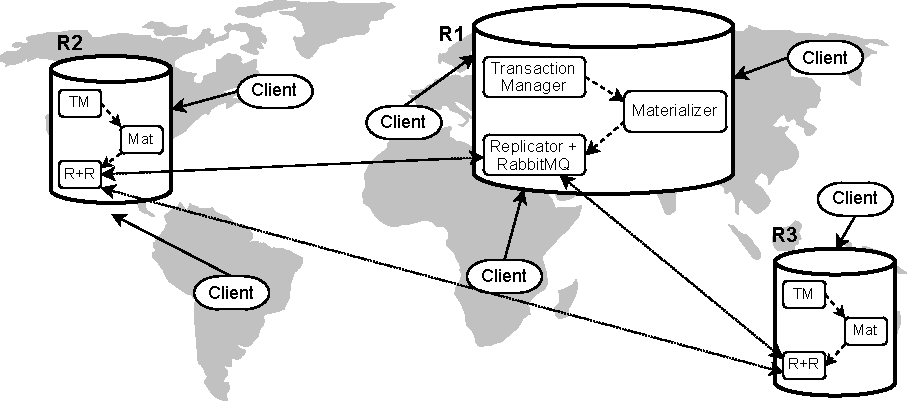
\includegraphics[width=\linewidth]{PotionDBArch}
	\caption{PotionDB Architecture}
	%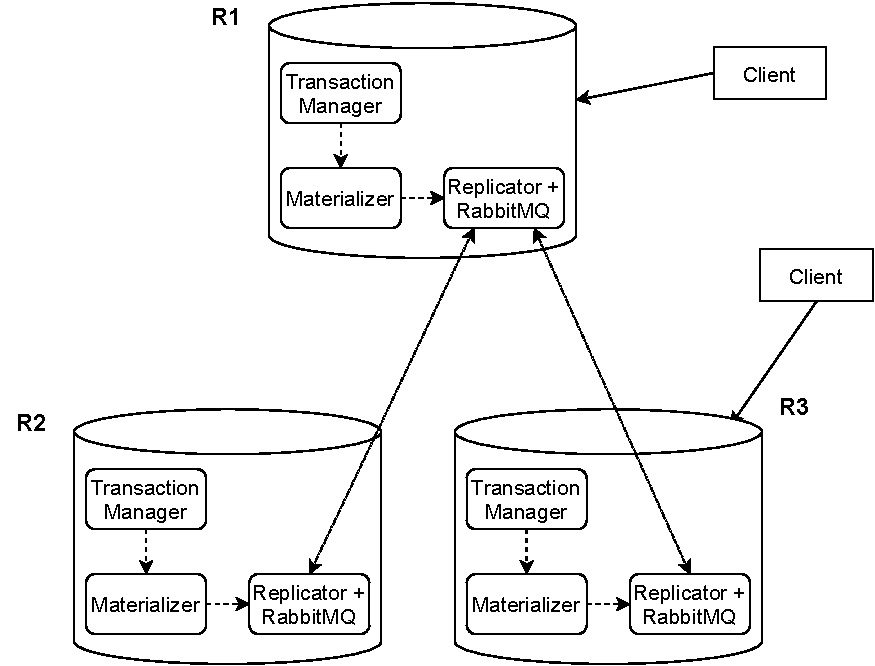
\includegraphics[width=.95\linewidth]{potiondb_architecture}
	%\caption{PotionDB Architecture~\carla{wasted space}}
	\label{fig:arch}
\end{figure}

We designed PotionDB with geo-replication in mind.
Thus, we assume PotionDB instances are spread across the globe (Figure \ref{fig:arch}).
Each instance only replicates a subset of the whole datastore's data.
The system administrator has control over where each object is replicated.
This allows to account for data locality to ensure fast access to data, while keeping replication and storage costs in check.
Objects without locality on their access pattern can be replicated everywhere if desired.
We detail this more in Section \ref{sec:replication}.

%I think details on how transactions work and guarantees do not belong here. So this is OK (but still needs to be explained somewhere).
Clients communicate with the nearest PotionDB instance to ensure low latency.
A client's transactions are locally executed in the PotionDB's instance the client is connected to.
Updates are propagated asynchronously to other replicas.
If a client's transaction accesses objects not locally replicated, other instances with said objects are contacted and involved in the transaction.
We note this should be an exceptional case, not the norm.
We leave further details for Section \ref{subsec:operationsNonLocal}.

The internal architecture of PotionDB is inspired by Cure~\cite{cure} and is split into three main components:

%Not sure if I'll need these abbreviations later. Consider removing if unused.
\begin{compactitem}
	\item TransactionManager (TM). This component is responsible for receiving and replying to client's requests.
	It coordinates transactions, implementing a transactional protocol (details shown in Section \ref{sec:transactions}) which ensures the consistency of reads and updates, as well as transactions' atomicity.
	\item Materializer: This component stores the objects on their latest version, alongside the necessary data to generate previous versions when necessary.
	Garbage collection keeps the amount of metadata in check.
	\item Replication: This component ensures that committed transactions are replicated asynchronously to other PotionDB instances.
	It is also responsible for receiving remote transactions and forwarding them to the TransactionManager for local execution.
	The replication component is aware of each instances' replication scheme, ensuring each one only receives updates for objects it replicates. We detail this in Section \ref{subsec:partial}.
\end{compactitem}

\subsection{CRDTs}
\label{subsec:CRDTs}
%Maybe CRDTs should go to a "Background" section. If we ever have that, Consistency can likely go there too.
%Should I mention the CRDTs we implement are the op-based ones? I will mention that in Replication.

PotionDB's objects and views are implemented as CRDTs \cite{crdt}.
CRDTs, Conflict-free Replicated Data Types, are a group of data structures which ensure concurrent updates do not conflict and that the state of all replicas eventually converges, assuming all updates are eventually delivered.
Many kinds of CRDTs have been proposed in the literature, forming a rich library of object types, e.g., counter, register, flag, set, map and topK (leaderboard).  \carla{maybe topK needs to be further explained}
Instead of direct assignments, CRDTs support rich operations to directly modify an object’s existing state, e.g., an increment on a counter.
Thus, application developers can pick the CRDTs corresponding to the data types appropriate for their application(s), without having to worry on how to handle concurrency conflicts.
CRDTs, together with our transactional causal consistency support and provisioning of snapshots (Section \ref{sec:consistency}), ease the life of application developers, as they will encounter less anomalies compared to other weak consistency solutions.
This avoids the need for ad-hoc mechanisms that are error-prone to compensate anomalies \cite{crdt, cure, bayou, coda}. \carla{check refs 17, 18, 22, 23 on the paper Composition in State-based Replicated Data Types}

In PotionDB we support the following data types: counters, registers, sets, maps, topK, average and max/min.
Our CRDTs support multiple operations and reads which ease their usage. 
E.g., in a map, both single and group additions/removals can be executed; for reads, the whole map can be read, directly check if a certain key exists or get the value of a key.
We further extended some CRDTs designs to make them more expressive.
E.g., our topK supports both additions and removals, as well as extra fields necessary to answer queries; we also provide topSum, a variant of topK, which supports incrementing or decrementing an existing entry.
Our maps are composable, i.e., the value of a map can be any other CRDT, which further enhances the expressiveness of PotionDB.
%Does the composability need some example to justify it?

These extensions and multi-operations, as well as the variety of data types, makes CRDT's implementation in PotionDB cumbersome, as it is necessary to ensure the states converge despite the execution of concurrent operations, as well the sequential semantics of the object is respected. \carla{Is the sequential semantics of CRDTs something well-known?}
It is also necessary to support efficient replication of each CRDT's updates.
We also had to support version management for each CRDT in order to provide our casually consistent snapshots.
However, our efforts allow us to efficiently support complex OLAP queries. %Should I refer again it eases application developer's lifes?
For instance, we fully implemented TPC-H's dataset and update operations in PotionDB.
Furthermore, using PotionDB's view API, we have defined efficient, automatically maintained views for each query in TPC-H.
Said views utilize many of PotionDB's data types, which showcases the expressiveness of PotionDB's API and data types.
%For instance, we implemented the TPC-H's \cite{tpch} dataset, update operations and six of their queries, including defining efficient, maintainable views for each query.
%We also analysed the remaining queries and sketched solutions for implementing all remaining queries using PotionDB's objects and views, which demonstrates PotionDB's expressivety. %Maybe I should say data types instead of "objects and views"?
We leave details on our TPC-H implementation for Section \ref{sec:views_for_apps}.
%Do I need to refer here that I explain NuCRDTs (or non-uniform replication) in another section?
%Should I explain here in detail our extensions to TopK and TopSum? May be a bit difficult to explain the later here without explaining non-uniform replication.

%New view: top 10 of customers with highest value sales. So it's like a top and a sum too.
%Or can still keep the TopSales but maybe instead have all the information needed be on the sales table. Can always explain the advantage with how the information can be split across servers

\subsection{View API}
\label{subsec:viewAPI}
%TODO: In other sections I may have to update where it says things like "how views are updated is agnostic to our solution" and similar. This is present likely in transactions and replications' sections. Since now we do provide a way to take care of update generation automatically.

PotionDB's materialized views can speed up the execution of queries by aggregating and  summarizing data partitioned across multiple servers, without a single server containing all the information required for the view.
With a simple read on a view, complex OLAP queries over global data can be quickly served, while still making full usage of data locality to save on replication costs.

Defining materialized views by directly composing PotionDB's data types, while possible, can be quite complex and cumbersome.
This is further aggravated by the need to keep views updated, which would require the application developer to write code for updating both the base objects and views.

To ease the deployment of views, we define and provide a specification language inspired in SQL \cite{sequel}.
By utilizing this language, the programmer can define views with ease, as PotionDB automatically infers the objects needed to support the view, as well as generate the required view updates whenever a relevant base object is inserted, updated or deleted. 
%To avoid this, we specify a language inspired in SQL \cite{sequel} to specify materialized views.
%From this specification, PotionDB can automatically infer the required objects to support the view, as well as automatically generate the necessary view updates' whenever a relevant base object is inserted, updated or deleted.
We detail this automated process in Section \ref{subsec:generated_view}.
Generated views are read in the same way as any other object (check Table \ref{table:PotionDB_API}).
%Note that the API to read a view's state is the same as the one previously described to read other objects.
%Updating or reading a view is done with the same interface used for other objects, as described in Section \ref{subsec:CRDTs}.
%Details on how we keep a view up-to-date and consistent with the objects it builds upon is left for Sections \ref{subsec:viewsTransaction} and \ref{subsec:repl_views}.
%As such in this section we focus on how can a view be specified, namely how to make it depend on the state of other objects.

\begin{table}[t]
	\setlength\tabcolsep{3.5pt}
	\small
	\begin{minipage}{0.5\textwidth}
		\centering
		\begin{tabular}{llllll}
			\multicolumn{6}{c}{\textbf{Sales}} \vspace{0.4em} \\%\hline
					\hline
			\multicolumn{1}{|l|}{ID} & \multicolumn{1}{l|}{ProdName} & \multicolumn{1}{l|}{Customer} & \multicolumn{1}{l|}{Price} & \multicolumn{1}{l|}{Cost} & \multicolumn{1}{l|}{SaleDate} \\ \hline
			\multicolumn{1}{|l|}{1}  & \multicolumn{1}{l|}{Laptop}      & \multicolumn{1}{l|}{Bob}      & \multicolumn{1}{l|}{1200}       & \multicolumn{1}{l|}{500} & \multicolumn{1}{l|}{28/01/23} \\
			\multicolumn{1}{|l|}{2}  & \multicolumn{1}{l|}{Phone}      & \multicolumn{1}{l|}{Bob}      & \multicolumn{1}{l|}{350}       & \multicolumn{1}{l|}{100} & \multicolumn{1}{l|}{07/02/23} \\
			\multicolumn{1}{|l|}{3}  & \multicolumn{1}{l|}{Laptop}      & \multicolumn{1}{l|}{Alice}      & \multicolumn{1}{l|}{1200}      & \multicolumn{1}{l|}{500} & \multicolumn{1}{l|}{10/02/23} \\
			\multicolumn{1}{|l|}{4}  & \multicolumn{1}{l|}{Phone}      & \multicolumn{1}{l|}{Alice}      & \multicolumn{1}{l|}{350}       & \multicolumn{1}{l|}{100} & \multicolumn{1}{l|}{13/02/23} \\
			\multicolumn{1}{|l|}{5}  & \multicolumn{1}{l|}{Disk}      & \multicolumn{1}{l|}{Charlie}      & \multicolumn{1}{l|}{100}        & \multicolumn{1}{l|}{20} & \multicolumn{1}{l|}{15/02/23} \\ 
			\multicolumn{1}{|l|}{6}  & \multicolumn{1}{l|}{Phone}      & \multicolumn{1}{l|}{Bob}      & \multicolumn{1}{l|}{350}       & \multicolumn{1}{l|}{100} & \multicolumn{1}{l|}{16/02/23} \\
			\multicolumn{1}{|l|}{7}  & \multicolumn{1}{l|}{Disk}      & \multicolumn{1}{l|}{Bob}      & \multicolumn{1}{l|}{100}       & \multicolumn{1}{l|}{20} & \multicolumn{1}{l|}{16/02/23} \\ \hline
		\end{tabular}
		\vspace{1em}
		\captionof{table}{\textit{Sales} table.}
		\label{table:sales}
	\end{minipage}
\end{table}

\begin{figure}
	\setlength\tabcolsep{3.5pt}
	\begin{minipage}{0.19\textwidth}
		\small
		\begin{tabular}{lll}
			\multicolumn{3}{c}{\textbf{TopSales}} \vspace{0.4em}        \\
			\hline                                               
			\multicolumn{1}{|l|}{Customer}   & \multicolumn{1}{l|}{Profit} & \multicolumn{1}{l|}{NSales} \\ \hline
			\multicolumn{1}{|l|}{Alice} & \multicolumn{1}{l|}{950}     & \multicolumn{1}{l|}{2}        \\
			\multicolumn{1}{|l|}{Bob}  & \multicolumn{1}{l|}{580}      & \multicolumn{1}{l|}{3}        \\
			\multicolumn{1}{|l|}{Charlie}   & \multicolumn{1}{l|}{80}      & \multicolumn{1}{l|}{1}        \\ \hline
		\end{tabular}
		\vspace{1em}
		\captionof{table}{\textit{TopSales} materialized view for February. This view builds upon \textit{Sales} objects.}
		\label{table:topSales}
	\end{minipage} \hfill
	\begin{minipage}{0.27\textwidth}
	\begin{lstlisting}[language=SQL]
CREATE VIEW (key, bucket) AS
SELECT attribute1, ..., attributeN
FROM container
WHERE condition(s) 
[ORDER BY ... ]
[LIMIT ...]
		\end{lstlisting}
		\captionof{figure}{Specification of views in PotionDB}
		\label{fig:viewSQL}
	\end{minipage}
\end{figure}

\begin{figure}[t]
\begin{lstlisting}[language=SQL]
CREATE VIEW (TopSales, views) AS 
SELECT ProdName sum(Price - Cost) AS SumProfit
	      count(sales.ID) AS NumSales 
FROM sales 
WHERE SaleDate.Month == [MONTH] and SaleDate.Year == 2023
ORDER BY SumProfit DESC, NumSales DESC 
LIMIT 10
\end{lstlisting}
	\caption{Specification of the view \emph{TopSales}.}
	\label{fig:topSalesSQL}
\end{figure}

Figure \ref{fig:viewSQL} showcases the aforementioned language.
Clause \qcr{CREATE} defines the key and bucket of the view.
The type is automatically inferred from the specification.
Clause \qcr{FROM} defines which objects to use to build the view, and \qcr{SELECT} chooses which attributes of the objects should be used for the view.
The attributes for the view can potentially be one of the following aggregating functions of objects' attributes: \qcr{sum}, \qcr{count}, \qcr{max}, \qcr{min}, \qcr{avg}.
Clause \qcr{WHERE} allows to define conditions that are used to decide whenever a given object is considered for the view or not, depending on certain attributes of the object (e.g., only include European customers in the view).
Clause \qcr{ORDER BY} sorts the rows of the view given one or more attributes of the view.
Lastly, \qcr{LIMIT} indicates that this view represents a top, i.e., a leaderboard, and optionally defines a maximum number of elements to be considered as being in the top.

Any parameter of the intended query should be indicated between []. 
For conditions in \qcr{WHERE}, usual comparison operators are supported, as well as operations over strings (e.g., \qcr{startsWith}). %Should we mention in theory we could support directly comparing dates?
Simple conditional expressions are also supported inside aggregates, to further boost the language expressiveness.	%This is useful e.g. for Q14, that way we can use one single average object instead of two.

%Now explain from.
In PotionDB we have objects instead of tables.
Thus, to provide a ``table-like'' vision, we assume the objects can be organized in containers - e.g., we could define that all objects representing customers are in a \emph{customers} container.
The \qcr{FROM} clause then refers to one (and only one) container. %\footnote{PotionDB actually supports more than one container in \emph{From}, as long as each object from the first container matches exactly one object of each of the remaining containers. We discuss this further in Section \ref{subsec:limitations}.}. 
This abstraction allows for a view to easily refer to objects as if they were organized in tables, as well as consider objects that have not yet been created.
Objects in the same container can still be in different buckets, e.g., have a bucket for each country and have each customer associated to its home country's bucket.
Thus, views can refer to objects that are not replicated in the local server.
We assume an object's container is non-mutable. %Do I need to refer anything further about containers (e.g. that they have no implications on implementation?)
\carla{Buckets where not introduced yet.}

%Note: Is the explanation below necessary? I believe it is not. Probably would be enough to say that table contains an example of a materialized view.
%The explanation is a bit difficult since none of this maps to actually anything in the implementation...
Figure~\ref{fig:topSalesSQL} shows the specification of a view which answers the following query: \emph{``Who were the top 10 most profitable customers on any given month of 2023? And, for each of the top clients of said month, how many products did each client buy?"}
Example data of the base objects and view can be seen, respectively, in Tables~\ref{table:sales} and \ref{table:topSales}.
Such a query can be useful to identify customers to which to direct special promotions in order to keep them as regular customers, as well as identify if high profit customers tend to buy many cheap products or few but expensive ones.
%Such a query can be useful to identify products that may need to be restocked, see if promotions/advertisement were effective, etc.
%This view is implemented with a topSum CRDT, taking data from all products and sales, as specified in \emph{From}.

The \qcr{FROM} clause specifies that all objects belonging to the container \emph{Sales} should be considered, while \qcr{SELECT} lists which attributes should be part of the view.
The \qcr{WHERE} clause ensures only sales done on 2023 are considered, with the parameter \qcr{[MONTH]} ensuring the results are separated per month.
Thus, the user can query the view to obtain the top sales for any desired month of 2023.
Meanwhile, \qcr{ORDER BY} defines how to sort the rows, using attribute \qcr{NumSales} as a tie-breaker, while \qcr{LIMIT} specifies how many elements are considered to be ``in the top".
More complex queries are also possible, namely, our specification language allows specifying efficient views for most of TPC-H's queries - out of TPC-H's 23 queries, we managed to specify views for 20 queries using our language.

%I think the extension below is not hard to do - it is just a very restricted form of join, as it must be a 1:1 match. But helps in many cases. What I still need to think about, is how to include that in the specification language in a way that it is clear.
%Implementing is not too complicated as it should be a simple GET of the primary key.
\emph{\textbf{Extensions.}} We extend the specification language as follows.
On the \qcr{FROM} clause, multiple containers are supported, as long as each object from the first container matches, through condition(s) defined in \qcr{WHERE}, exactly one object of each of the other containers.
This allows for views to fetch data that may be in other objects that are relevant for the view.
E.g., in the TopSales, we could fetch the customer's nation from the customer's container.

We also provide an alternative interface for views which gives the application developer more control over the created views.
The application developer can specify a trigger (i.e., code) that is run on the database to generate updates for views.
Each trigger is associated to a container and an event (new, update or delete object) and can generate updates for one or more views.
Each time the respective event regarding objects of said container occurs, the trigger's code is executed.
Any updates generated by the trigger are appended to the current transaction.
The trigger can, if needed, read the local objects and see all updates in the transaction. %Idea: can define a trigger on a "new order" but that trigger accesses the new items being added in the same transaction.
This mechanism allows to specify some views not possible with our view API, further extending the possibilities of views in PotionDB.
For instance, by using triggers, all queries in TPC-H can be served efficiently with views in PotionDB.

%%%%%%%%%%%%%%%%%%%%%%%%%%%%%%%%%%%%%%%%%%%%%%%
%%%%%%%%%%%%%%%%%%%%%%%%%%%%%%%%%%%%%%%%%%%%%%%
%%%%%%%%%%%%%%%%%%%%%%%%%%%%%%%%%%%%%%%%%%%%%%%
%%%%%Incomplete sections written by Nuno. I tried to use this as a base.%%%%%
%Some parts were moved to other Sections, e.g., to Consistency and Transactions
\if 0
\subsection{Data model}

PotionDB a key-value database,  where values can be base objects, $Objs$,  or derived objects,
$Views$, with $DB = Objs \cup Views$. For simplicity of presentation we consider that the key is a property of
the object and say that the database, $DB$, is composed by a set of objects, $DB = Objs \cup Views$. 
When needed, we represent the key of object $o \in DB$ as $o^{key}$.

The value of a derived object is defined as a function of the value of other database objects, i.e.,
$\forall v \in Views, v=fun_v(D_v)$, with  $D_v$ the set of database objects used to compute $v$.
We assume the computation is non-recursive, i.e., the value of an object is never a function of its own value, 
$\forall v \in Views, v \not \in dom(v)$, with $dom(v)$ the set of objects used, directly or indirectly, to 
compute the value of $v$.

\subsubsection{Data Access}

Database objects have a type and provide an interface with read and update operations, 
where read operations do not change the value of the database and update operations change
its value. Applications access the database by executing transactions, which are sequences of
read and update operations. 

\begin{figure}[h]
\begin{lstlisting}
begin() $\rightarrow$ txId
commit( txId)  $\rightarrow$ ok | error
rollback( txId)

get( txId, id) $\rightarrow$ value
read( txId, id, op) $\rightarrow$ value
update( txId, id, op) $\rightarrow$ value
\end{lstlisting}

\caption{PotionDB data access API.}\label{fig:dataapi}
\end{figure}

Figure~\ref{fig:dataapi} presents the API provides for data access. Th




an interface with a set of operations, 








\andre{I repeated the uid explanation from Database Model and API to here... where should it stay?}

PotionDB provides a key-value store interface with support for transactions.
Objects are uniquely identified (uid) by the triple (key, bucket, type), where key is a user provided name for the object, bucket identifies where the object should be replicated and type is the type of object.
We support both \emph{read} and \emph{update} operations on an object, as well as operations to \emph{start}, \emph{commit} and \emph{abort} transactions.
More precisely, said operations have the following format:

\firstblockemph{get(uid) $\rightarrow$ object}

\middleblockemph{read(uid, op, params) $\rightarrow$ data}

\middleblockemph{update(uid, op, params))} \\

\middleblockemph{beginTx(startTs)}

\middleblockemph{commitTx()}

\lastblockemph{abortTx()}

We now explain the arguments of each operation and the expected result.
\andre(Any suggestions for a better phrase here...?)

\emph{get(uid) $\rightarrow$ object}. Given an object identified by \emph{uid}, it returns the state of the object.
E.g., in a set, it returns all the elements in the set.

\emph{read(uid, op, params) $\rightarrow$ data}. Performs a partial read in the object identified by \emph{uid}, returning the result of said read. 
\emph{Op} identifies the type of read operation to apply, while params correspond to the arguments necessary (if any) for that read operation.
E.g., in a set, emph{get(uid, lookup, ``e'')} returns \emph{true} if the set identified by uid contains the element ``e'', \emph{false} otherwise.

\emph{update(uid, op, params)}. Applies an update to the object identified by \emph{uid}, modifying its state.
\emph{Op} and \emph{params} have the same meaning as in \emph{read()}.
E.g., in a set, \emph{update(uid, add, ``e'')} adds the element ``e'' to the set identified by uid.

\emph{beginTx(startTs)}. Starts a new transaction. Optionally, a starting timestamp \emph{startTs} can be supplied. This ensures that a client will not read older versions when contacting a different replica from where he executed his previous operations.
\andre{TODO: Add reference to some place where I explain this properly...?}

\emph{commitTx()}. Commits a transaction, applying the effect of every update operation issued since the respective \emph{beginTx}.

\emph{abortTx}. Cancels a transaction, ensuring the updates issued since the respective \emph{beginTx} have no effect.

\andre{I think somewhere I'll have to explain the following: a) how beginTx works when receiving a startTs; b) how are commits/aborts handled (i.e., when updates are applied); c) that reads return right away and consider the temporary effects of updates issued in that transaction}




\subsection{System model}

We consider a system composed by $n$ sites, with $R = \{r_1,\ldots,r_n\}$ the set
of sites (where each site is typically a data center).
Each database object is replicated in a 
subset of the sites, i.e., $\forall o \in DB, Reps(o) \subseteq R$, with $Reps(o)$ the set
of the sites that replicate $o$.





\subsection{System model}


Applications access the database by issuing transactions. A transaction starts with a \texttt{begin} operation, 
and contains a sequence of read and update operations 

is a sequence of operations,
strating with %\teg




given  $fun_v$ the function used to compute the value of $v$ and $dom(v)$ the set of database objects used



given  $fun_v$ the function used to compute the value of $v$ and $dom(v)$ the set of database objects used
to compute the value of $v$, $\not \exists v_i \in dom(v): v \in dom(v_i)$.

 
$\forall v \in Views, \exists D_v \subset DB, v = fun_v(D_v)  \wedge $, with $fun_v$ the function used to compute 
the value of $v$. 

here the values of the database used to compute 


 $fun_v$ can be computed without .


Typically 

The database additionally contains a set of derived objects, or views, $Views$, where each 

 

We consider a database composed by a set of objects partially replicated in
multiple data centers.
The code of an operation executes a sequence of reads
and updates enclosed in a transaction.
As the transaction executes in an initial replica, the effects of updates are 
recorded and queued for replication upon transaction commit.
The propagation of updates can be asynchronous and must respect causal order.
Hereafter, we use the term operation to refer the updates produced by the 
execution of the transaction code in the initial replica.

We denote by $o(S)$ the state after applying the updates of
operation $o$ to state $S$.
A database snapshot, $S_n$, is the state of the database after
executing a sequence of operations $o_1,\ldots,o_n$
in the initial database state, $S_{init}$, i.e., $S_n =
o_n(\ldots(o_1(S_{init})))$.
The set of operations reflected in snapshot $S$ is denoted by $Ops(S)$,
e.g., $Ops(S_n) = \{o_1,\ldots,o_n\}$.
The state of a replica results from applying both local and remote
operations, in the order received.

%\textls[-25]{
We say that an operation $o_a$
%that executed initially in the database snapshot $S_a$
happened-before operation $o_b$ executed initially in  database snapshot $S_b$,
$o_a \! \prec o_b$ iff \mbox{$o_a \in Ops(S_b)$}.
Operations $o_a$ and $o_b$ are concurrent, $o_a \! \parallel \! o_b$ iff
$o_a \!\not \prec o_b \! \wedge \! o_b \!\not \prec \! o_a$ \cite{happensbefore}.
%}

For an execution of a given set of operations $O$, the happens-before relation defines
a partial order among operations, \mbox{$\mathcal{O} = (O,\prec)$}.
We say $\mathcal{O'} = (O,<)$ is a valid serialization of $\mathcal{O} = (O,\prec)$
if $\mathcal{O'}$ is a linear extension of $\mathcal{O}$, i.e., $<$ is a total order
compatible with $\prec$.

Operations can execute concurrently, with each replica
executing operations according to a different valid
serialization.
To guarantee state convergence, we assume the system gives the programmer 
the choice of various deterministic conflict resolution policies
on a per-object basis, i.e., the result of
applying updates that were executed concurrently is deterministic
independently of the execution order.
In our prototype, we rely on CRDTs
\cite{crdt,walter} to achieve this goal.

We consider that application correctness can be expressed in
terms of invariants \cite{bailisiser,indigo,cise}.
An invariant is a logical condition expressed over the database
state.
A given state $S$ preserves an invariant $I$ iff $I(S) = \mathit{true}$,
where $I(S)$ is a function that checks the validity of the invariant in state $S$.
A state $S_i$ is \emph{I-valid} (or simply valid) iff $I(S_{i}) = \mathit{true}$; otherwise the state is
\emph{I-invalid} (or simply invalid).
We require the initial state, $S_{init}$, to be valid.

We say that $\mathcal{O'} = (O,<)$ is an I-valid serialization of \mbox{$\mathcal{O} = (O,\prec)$}
if $\mathcal{O'}$ is a valid serialization of $\mathcal{O}$, and $I$ holds in every state that
results from executing any possible prefix of $\mathcal{O'}$.
If $I$ is the conjunction of all application invariants, then we say that
an application is correct if, in any possible execution of that application,
every replica evolves through a sequence of I-valid states.
We say that an operation $o_1$ conflicts with $o_2$ if the execution of
$o_1$ makes the preconditions of $o_2$ false in some database state.





\subsection{Data Definition API}
\label{subsec:old_dataAPI}

As previously mentioned, PotionDB provides support for partial replication.
As such, it is essential to have a mechanism to choose which servers should replicate each object.

All objects in PotionDB have a ``bucket'' associated to it.
Buckets define groups of objects that are replicated in the same subset of replicas. In other words, two objects with the same bucket value will be replicated in the same set of replicas.
For each replica, the system admin can define which buckets will be replicated in it.

To exemplify, recall the e-commerce example described in Section \ref{sec:overview}.
The customers can be partitioned based on their country's continent by taking the following steps: 

\begin{enumerate}
	\item Define one bucket per continent;
	\item Configure the servers so that each replica replicates the bucket of its continent (+ possibly others for fault tolerance);
	\item When adding a customer to the database, specify the bucket correspondent to the customer's continent.
\end{enumerate}

We leave details on the internal workings of our replication algorithm, namely how it ensures each object is only sent to the right subset of replicas, to Section \ref{subsec:replication}.

%Section \ref{subsec:replication} gives more details on how PotionDB handles replication, namely how it ensures each object is only sent to the right subset of replicas.

%It's worth noting that clients must ensure they are communicating with a server which replicates the buckets they want to operate on, since each server only replicates a subset of the buckets and doesn't forward operations to other servers.

%(será aqui??)
%apresentar como se define a que partição pertence cada objeto.


\subsection{Data Access API}

\andre{I repeated the uid explanation from Database Model and API to here... where should it stay?}

PotionDB provides a key-value store interface with support for transactions.
Objects are uniquely identified (uid) by the triple (key, bucket, type), where key is a user provided name for the object, bucket identifies where the object should be replicated and type is the type of object.
We support both \emph{read} and \emph{update} operations on an object, as well as operations to \emph{start}, \emph{commit} and \emph{abort} transactions.
More precisely, said operations have the following format:

\firstblockemph{get(uid) $\rightarrow$ object}

\middleblockemph{read(uid, op, params) $\rightarrow$ data}

\middleblockemph{update(uid, op, params))} \\

\middleblockemph{beginTx(startTs)}

\middleblockemph{commitTx()}

\lastblockemph{abortTx()}

We now explain the arguments of each operation and the expected result.
\andre(Any suggestions for a better phrase here...?)

\emph{get(uid) $\rightarrow$ object}. Given an object identified by \emph{uid}, it returns the state of the object.
E.g., in a set, it returns all the elements in the set.

\emph{read(uid, op, params) $\rightarrow$ data}. Performs a partial read in the object identified by \emph{uid}, returning the result of said read. 
\emph{Op} identifies the type of read operation to apply, while params correspond to the arguments necessary (if any) for that read operation.
E.g., in a set, emph{get(uid, lookup, ``e'')} returns \emph{true} if the set identified by uid contains the element ``e'', \emph{false} otherwise.

\emph{update(uid, op, params)}. Applies an update to the object identified by \emph{uid}, modifying its state.
\emph{Op} and \emph{params} have the same meaning as in \emph{read()}.
E.g., in a set, \emph{update(uid, add, ``e'')} adds the element ``e'' to the set identified by uid.

\emph{beginTx(startTs)}. Starts a new transaction. Optionally, a starting timestamp \emph{startTs} can be supplied. This ensures that a client will not read older versions when contacting a different replica from where he executed his previous operations.
\andre{TODO: Add reference to some place where I explain this properly...?}

\emph{commitTx()}. Commits a transaction, applying the effect of every update operation issued since the respective \emph{beginTx}.

\emph{abortTx}. Cancels a transaction, ensuring the updates issued since the respective \emph{beginTx} have no effect.

\andre{I think somewhere I'll have to explain the following: a) how beginTx works when receiving a startTs; b) how are commits/aborts handled (i.e., when updates are applied); c) that reads return right away and consider the temporary effects of updates issued in that transaction}


%\begin{verbatim}
%begin_tx()
%commit_tx()
%rollback_tx()
%
%get( key) -> object
%readOp( key, op, params) -> data
%updateOp( key, op, params)
%\end{verbatim}
%
%Explicar o que são - isto ém qual o resultado esperado.


\subsection{View Definition API}
\label{subsec:old_viewAPI}

PotionDB supports materialized views, which can speed up the execution of certain queries by summarizing data spread across multiple objects.
The data referred by a view does not need to be all replicated in a single server - such data can be partitionated across multiple servers.

Views can be read the same way as non-view objects, by using the same \emph{get} and \emph{read} interface.
On the other hand, updates work differently - PotionDB automatically updates views by using user supplied \emph{triggers}.
A view object is created when the first read, or an update generated by a trigger, is defined for it.

We support the following type of views:
\begin{itemize}
	\item max, min, sum, average: aggregation functions used to summarize information from usually multiple counter objects;
	\item topK/leaderboard: keeps a list of the \emph{n} elements with highest score. That is, a list of pairs (id, score) ordered from highest to lowest score. In practice, this implements the functions \emph{limit} and \emph{orderby}. An example of this view can be the top 100 customers with highest spendings in a store.
	\item common types of objects like counters, registers, sets and maps can be used as views. E.g., it is possible to have a counter which keeps track of how many times a given object was modified.
\end{itemize}

As referred, views are updated automatically by making use of user-supplied triggers.
The intuition behind triggers is to automatically generate updates to views, by defining how updates on certain objects translate into updates on views.
\andre{How do I refer that this is a common practice too in relational databases?}
We extend our key-value store API presented before with the following operation, in order to support the definition of triggers:

\firstblockemph{Create Trigger name}

\middleblockemph{On uid1}

\middleblockemph{With operationName1(arguments)}

\middleblockemph{Do Update uid2}

\lastblockemph{With operationName2(arguments)}

\emph{Create Trigger name} specifies the name associated to this trigger, so that it can later be removed if needed.
\emph{On uid1} specifies the object that activates this trigger, while \emph{with operationName1(arguments)} specifies the type of operation, as we may want a trigger to only be fired on, e.g., adds.
\emph{Do Update uid2} specifies the object (view) which will be updated by the trigger, while \emph{with}  \emph{operationName2} \emph{(arguments)} specifies which operation will be applied on the view.

A simple example would be:

\firstblockemph{Create Trigger t1}

\middleblockemph{On (key1, bucket, COUNTER)}

\middleblockemph{With inc(c)}

\middleblockemph{Do Update (key2, bucket, REGISTER)}

\lastblockemph{With set(c)}

With this trigger, everytime an increment (but not decrements) is applied to the counter identified by (key1, bucket, COUNTER), an update is created for the register object identified by (key2, bucket, REGISTER).
The value used to increment the counter (argument \emph{c}) is then used to update the register.
In practice, this makes the register keep track of the latest increment applied to the counter.

It is also possible to define more generic triggers that are fired whenever a subset of objects are updated.
This is done by allowing the key and bucket of uid1, i.e., the object that triggers, to be a regular expression.
We support the RE2 \cite{RE2sintax} sintax for regular expressions.

To exemplify a generic trigger, consider that we have multiple counter objects identified by (counter1, bucket, COUNTER), (counter2, bucket, COUNTER), ..., (counterN, bucket, COUNTER), along with one topK object identified by (topk1, bucket, TOPK).
Assume our goal is for the topK to register the maximum increment of each counter.
One way of achieving this is by defining the following trigger:

\firstblockemph{Create Trigger t2}

\middleblockemph{On (counter[0-9]\textsuperscript{+}, bucket, COUNTER)}

\middleblockemph{With inc(c)}

\middleblockemph{Do Update (topk1, bucket, TOPK)}

\lastblockemph{With add(counter[0-9]\textsuperscript{+}, c)}

In this particular case, any object that simultaneously meets the requirements of
\begin{enumerate*}[label=(\roman*)] 
	\item being a counter; 
	\item belonging to the bucket \emph{bucket};
	\item key starts with \emph{counter}, followed by one or more numbers;
\end{enumerate*}
will trigger an update to the topK whenever an increment is applied.
The key of the counter object is used for the id of the entry in the topK.

\andre{I added this new paragraph to explain @ custom code}.

More complex queries may require a view which needs multiple steps or intermediate calculations to update.
For such scenarios, the current implementation of PotionDB allows generic code to be associated to the trigger.
Ideally, a specific data manipulation language would be used for this purpose (e.g., \cite{oracleTriggers}), but this sits outside of the scope of the paper and is thus left as future work.
We leave further details on the inner workings of triggers, as well as views, to Section \ref{sec:views}.





\subsection{System API}



%\textbf{need better examples}.
%For instance, an asian customer is more likely to consult the stock of stores in his country rather than in an european country.
%Thus, it makes sense that both asian customers' and asian stores' data to be replicated mainly in asian data centers (plus possibility a subset of others for fault tolerance purposes).
%That is, the servers for which data will be replicated can be choosen based on the geographic location, as its relevance depends on such factor.




%=========================================================================================
%=========================================================================================
%=========================================================================================
%=========================================================================================
\if 0

\section{Motivation example}
\label{sec:example}

%TODO: I need to include here the complete example query. And explain why the tradicional way with key-value stores is non-efficient. And why a view theorically makes it both easier and more efficient.
%Use as a starting point the text in "Old stuff that may still be useful"

In order to both facilitate the understanding of the rest of the paper, as well as show the usefulness of queries supported by materialized views, we present the following example scenario.

Consider a large scale commerce company with stores and clients spread across the world.
Assume the company keeps data of millions of products, with each store having its own stock of products available.
Also consider that there are millions of both current and past customers and, among other data, all sales ever done are kept in the database, for both product warranty and statistical purposes.

Fully replicating the whole dataset would have proibitive costs.
It is also unecessary, as both the relevance of the data and likehood of being accessed from are dependent on the location.
For instance, an asian customer is more likely to consult the stock of stores in his country rather than in an european country.
Thus, it makes sence that both asian customers' and asian stores' data to be replicated mainly in asian data centers (plus possibility a subset of others for fault tolerance purposes).
That is, the servers for which data will be replicated can be choosen based on the geographic location, as its relevance depends on such factor.

To keep the example simple, we will only consider three types of objects: customers, products and sales.
The simplified scheme of each object can be found on Figure \ref{fig:objects}.

\begin{figure}
	%\begin{table}[]
	\centering
	\begin{tabular}{|l|l|}
		\multicolumn{2}{c}{Customer} \\ \hline
		id            & int          \\ \hline
		name          & string       \\ \hline
		age           & int          \\ \hline
		country       & string      \\
		\hline
	\end{tabular} \hspace{0.7em}
	\raisebox{0.225\height}{\begin{tabular}{|l|l|}
			\multicolumn{2}{c}{Products} \\ \hline
			id           & int           \\ \hline
			name         & string        \\ \hline
			value        & int   \\
			\hline       
	\end{tabular}} \hspace{0.7em}
	\begin{tabular}{|l|l|}
		\multicolumn{2}{c}{Sales} \\ \hline
		id            & int       \\ \hline
		custID        & int    \\ \hline
		productID     & int       \\ \hline
		amount        & int	\\
		\hline      
	\end{tabular}
	\caption{Example objects}
	\label{fig:objects}
	%\end{table}
\end{figure}

Customers represent clients that at some point in time have bought at least one product from one of the stores.
Products represents items that may be (or have been) for sale.
Sales represents the aquisition of one or more units of a product by a client, where custID and productID refer to, respectively, the customer's and product's id field.

For the purpose of this example, we'll consider the following replication scheme for each type of object:
\begin{itemize}
	\item \emph{Customer:} replicated in the data centers present in the continent correspondent to his country (plus a few other data centers for fault-tolerance purposes);
	\item \emph{Products:} replicated in all data centers;
	\item \emph{Sales:} replicated in the same data centers as of the customer who bought the product. 
\end{itemize}

Despite the fact that some objects aren't replicated everywhere, PotionDB will still support queries that refer to a global view of the database.
E.g., queries such as ``top 100 customers who have spent the most across all stores'' must be efficiently handled by PotionDB, even though no server contains all customer and sales data. 
This kind of queries allows to gather important real-time statistics which allow businesspersons to make decisions and changes on the business strategy to improve its rentability.
\andre{Should I refer tpc-h here?}

The following is an example of a query requiring a global view of the database:

\lineemph{Get the top 100 customers who have spent the most across all stores. For each customer, the name, age, country and total value spent must be returned.}

Without views and by using just the three kinds of objects in Figure \ref{fig:objects}, executing this query would require communication with multiple data centers across the world, as both sales and customers' data is partitioned.
Since there are millions of customers and sales records, this would imply downloading large amounts of data and also spending a considerable amount of CPU time for data joining.
After the joins are complete, it is still needed to calculate the total value spent for each customer and sort descendingly based on the total value spent by each customer.
Only after this whole process is complete can the query be answered correctly.
Due to the sheer amount of data involved, this query would have unnaceptable performance if executed in this way.

Defining the right view(s) avoids having to do for each query the process referred above.
For the example query above, a view that keeps, for each customer, his name, age, country and total value, ordered by total value, can answer efficiently the query with a single get operation.
With this we no longer need to contact multiple data centers and execute millions of gets and result processing.

On Section \ref{sec:views} we address multiple difficulties related to supporting and keeping views updated, as well as our solutions for such difficulties in PotionDB.

\fi
\fi
%=========================================================================================
%=========================================================================================
%=========================================================================================
%=========================================================================================


\section{{Consistency}}
\label{sec:consistency}

By default, PotionDB provides Transactional Causal Consistency (TCC).
We also support the weaker Read committed (RC) consistency. %Do I need to justify why we provide both? Basically the later is provided to achieve higher throughput.
We now detail the guarantees provided by PotionDB under both models.

\subsection{Transactional Causal Consistency}
\label{subsec:transactionalcausal}

%I introduce here the idea of snapshots. Maybe it should be before, e.g. Nuno had defined it in a draft of the system model.
%Maybe on Causality I should just use operation "a" and "b" like every other paper does... instead of "op1" and "op2"
%In VLDB, Paragraph is like another subsection - "10.1.0.1" doesn't look good, so I changed to \emph
\emph{Causality.} 
We leverage on the happens-before relationship defined by Lamport~\cite{lamport78} to define causality.
We represent that $op_1$ happened before $op_2$ as $op_1 \prec op_2$.
We can say that $op_1 \prec op_2$ iff any of the following conditions is true:

\begin{compactitem}
	\item Thread-of-execution: if $op_1$ and $op_2$ are operations in the same thread of execution (i.e., same client) and $op_1$ happens prior to $op_2$, then $op_1 \prec op_2$;
	\item Reads-from: if $op_1$ writes a value and $op_2$ reads the value written by $op_1$, then $op_1 \prec op_2$;
	\item Transitivity: if there is an $op_3$ such that $op_1 \prec op_2$ and $op_2 \prec op_3$, then $op_1 \prec op_3$.
\end{compactitem} 

We say two operations are casually related iff $op_1 \prec op_2$ or $op_2 \prec op_1$.
%By contrast, if neither condition is true, then the operations are concurrent.
By contrast, if $op_1 \nprec op_2$ and $op_2 \nprec op_1$, then $op_1 \parallel op_2$, i.e., are concurrent.

\emph{Causal Consistency.}
With causal consistency, it is required that the values observed by the clients respect causality.
Formally, given a read $r$ issued by a client, the result returned by $r$ must be the result of executing all write operations that preceed it according to the happens-before order.
As an example, if we assume a set and the operations $add(a)$ $\prec$ $add(b)$ $\prec$ $rem(c)$ $\prec$ $add(c)$ $\prec$ $rem(b)$, $r$ must return the set $\{a, c\}$, i.e., the result of executing the aforementioned operations according to the happens-before order.
%As an example, if we assume registers, $r$ must return the value written by the write that causally preceeds it.

If $op_1$ and $op_2$ are concurrent, they can be applied by any order.
Specifically, they may be executed by different orders in different replicas.
If both operations are a write for the same object, this could lead to replicas' state diverging forever \cite{cops, cure}, i.e., returning different results for the same read.
In this situation we say the writes are conflicting.
We assume in our model of causal consistency that some mechanism of conflict resolution is provided to solve conflicts in a per-object basis, i.e., that for any two conflicting writes the result is deterministic independently of the execution order.
In our solution, we leverage CRDTs to solve these conflicts~\cite{crdt}.
This model of causal consistency with a conflict resolution mechanism is referred by some authors as causal+ consistency \cite{cops, cure, chainreaction}.
We refer to this simply as causal consistency.
%I have to introduce CRDTs somewhere and "explain why they are wonderful" (API, automatic conflict resolution in different flavours, etc)

%I thought about referring to per-object and cross-object causality, and then saying we offer cross-object. But I couldn't find a way without making things more confusing or seem unecesary. I believe the rules we state in "Causality" already make it clear enough it is "cross-object", as rule 1 and 3 are generic enough to refer to different objects.
%If I need an example for cross-object being useful, check Eiger's paper, just before Section 4.1.

\emph{Transactional Causal Consistency.}
We extend the idea of causality to transactions.
In a transaction, it is desirable to have a consistent view of the database - i.e., observe a state where all the causality relationships are respected.
We define such a state as a snapshot.

Formally, we denote by $op(S)$ the state after applying the update(s) of $op$ to state $S$.
Let $S_{\mathit{init}}$ be the initial, empty state of the database.
We can define a snapshot $S_n$ as the state of the database after executing a sequence of operations $op_1, ..., op_n$ according to some valid serialization that respects the happens-before relationship, i.e., $S_n = op_1(...(op_n(S_{\mathit{init}})))$.
Since the serialization respects the happens-before relationship, $S_n$ is a consistent snapshot of the database.

%Try to avoid the repetion below.
All reads and updates of a transaction execute on top of a consistent snapshot, i.e., reads return the effects of $op_1, ..., op_n$ in $S_n$ and all updates happen after $op_1, ..., op_n$.
Our transactions are atomic and generate a new consistent snapshot when committed.
I.e., given any transaction $T$ executing on snapshot $S_n$ with operations $op_{t1}, ..., op_{tn}$, either $T$ commits and $S_t$ = $op_{tn}(...(op_{t1}(S_n)))$ (all operations on the new snapshot) or it aborts and $\forall\, op_{t} \in T : op_t \notin \mathit{Ops}(S_{t})$ (none of the operations are in the new snapshot, i.e., $S_{t}$ = $S_n$), where $\mathit{Ops}(S)$ denotes the list of operations that generated $S$ from $S_{\mathit{init}}$.
 
Our PotionDB prototype provides Transactional Causal Consistency (TCC) by default, i.e., our transactions always observe a consistent snapshot of the database.
Transactions are atomic, i.e., either all the effects of the updates in the transaction are reflected in the next state of the database or none are.

\subsection{Read committed}
\label{subsec:readcommitted}
%TODO: Maybe a table with all the symbols we use like in Cure?
%Note for self:  PotionDB does not provide repeatable reads under the weaker consistency model, because the same read during one transaction can return different values under Rc
Read committed (RC) is a consistency model which guarantees that only states resulting from committed transactions can be read.
This model provides weaker guarantees than transactional causal consistency.
However, on write-heavy scenarios (e.g., 75\%-25\% write-read workloads), the provision of consistent snapshots for TCC is expensive.
This is common problem for systems providing some sort of causal consistency.
E.g., Cure~\cite{cure}, Eiger~\cite{eiger}, GentleRain~\cite{gentlerain}, and COPS~\cite{cops} also have considerable performance drops when update ratios are high.
Thus, we provide RC for write-heavy scenarios where maintaining a high read throughput is a must.

Intuitively, under RC, PotionDB returns for each object the latest (committed) version available.
Thus, reads for different objects may return different versions.
This can be undesirable for some applications.
For example, if we want to access the data of a customer alongside his list of purchases, and assuming both informations are stored in two different objects, it is desirable to read both under TCC in order to observe a consistent state, as the objects are correlated.
%For example, if for a given product we have two different objects, one stating the number of sales and the other the total value of the sales, it is desirable to read both objects under TCC to observe a consistent state, as the objects are correlated.
However, for situations of reading unrelated objects or single objects, we argue RC is strong enough.
This scenario is somewhat common as we expect most complex queries in PotionDB to be served by a single view and, thus, a single read.
Besides, the application developer can always fall back to TCC whenever necessary.

We now define precisely our guarantees under RC.
First, consecutive reads of the same object either return the same state or a more recent state, whenever in the same transaction of not.
I.e., consider a transaction T, reads $R_1(o) \in T$ and $R_2(o) \in T$, as well as the states returned by them, respectively, $S_1(o)$ and $S_2(o)$.
Under RC, we have that $R_1(o) \prec R_2(o) \implies S_1(o) \prec S_2(o)$. \carla{I changed $s_i$ to $S_i$}
Thus causality on a single object is respected, but isolation from other transactions is not.
Under TCC, both reads would return the same state, while under RC, $S_2(o)$ could reflect changes from some other transaction that committed in the meantime.

Causality across objects is also not respected.
Assume $R_1(o_1) \in T$ and $R_2(o_2) \in T$, with $o_1^{id} \neq o_2^{id}$.
Under RC, the following is possible: $R_1(o_1) \prec R_2(o_2) \land S_2(o) \prec S_1(o)$.
I.e., reads of different objects may return states corresponding to different snapshots.

For two transactions $T_1$, $T_2$, with $T_1 \prec T_2$, there is still no causality across objects. However, for $R_1(o) \in T_1$, $R_2(o) \in T_2$, $S_1(o)$ $\prec$ $S_2(o)$.

\section{Transactions}
\label{sec:transactions}

PotionDB employs a transactional protocol in order to ensure the database's state evolves correctly and that transactions observe casually consistent snapshots.
This is necessary as internally PotionDB is sharded for performance, thus coordination is required.
Furthermore, our transactional protocol is also responsible for ensuring transaction's atomicity, as well as ensure views and their base objects are updated simultaneously and kept consistent.

In this section we describe PotionDB's sharding, our commit and reading protocols as well as how views are kept up-to-date with their base objects. %Do I need to make it clear the transactional protocol is commit + read?


%A table summarizing all symbols could be useful.
%Each PotionDB instance is internally sharded, as described in Section \ref{subsec:sharding}.
%Thus, to enable the provisioning of casually consistent snapshots of the whole database, coordination among partitions is required to execute transactions, ensuring state evolves correctly.
%If no coordination was employed it would be possible to observe inconsistent states of the database - e.g., observe a state where a base object is already updated but its base view is not. %I don't think I need to motivate this further... is it necessary to say this would lead to application errors/difficulties for the application developer, or that it would break transactional causal consistency?

%We define the following notation to help with our protocols definition in this section. %Maybe I should define a table for this like in Cure?
%Let $T$ be the current transaction being considered, $p_T$ the set of partitions for which there is a read or write in $T$, $p_{w(T)}$ the same but for writes only.
%Let $S_1, ..., S_n$ be the set of servers of the system.
%Let $clk^p_i$ be the value of the physical

\subsection{Sharding}
\label{subsec:sharding}

%Maybe I can mention doing sharding based on some other criteria (e.g., to make better usage of views + objects) is left as future work/orthogonal line of research.

Internally, the Materializer component (our datastore) is sharded.
This allows multicore CPUs to be efficiently utilized,
with reads and updates executing in parallel whenever possible.
Each object $o$ is assigned to only one shard, based on a hash of $o^{\mathit{id}}$.
For clarity, let $o^{\mathit{shard}}$ be the shard where $o$ is stored.
Each shard also has a unique id used for clock disambiguation.
For simplicity, it is also possible to obtain the shard of $o$ from its $id$, or from any read/update operation regarding $o$.

Each shard has one dedicated thread.
This avoids the usage of locks when accessing objects, simplifying the implementation and avoiding other issues such as lock contention.
It also allows for reads and updates on non-overlapping shards to execute in parallel.
In a way, our approach is similar to the one used in H-Store \cite{h-store}.
However, instead of running multiple instances of PotionDB and sharding the data across those instances, we shard the dataset across threads of the same database instance, as this allows for a more efficient communication between shards when necessary.
%Do I need to justify further the H-Store reference? 

%This needs us to define that we access the server with read() and update() before.
%The intuition is that in a given transaction, operations for different shards can execute concurrently without any conflict.
%For multiple transactions, if all transactions are read-only, then there is no conflict either as states do not change.
%However, when considering updates, if there is an overlap of updates of different transactions for the same shard, then there is a conflict, as the results may differ depending on the execution order.
%I am not sure if the "intuition" above is necessary at all.

Ideally, all transactions would execute concurrently at will, and long transactions would also execute concurrently across shards.
However, concurrent writes to the same shard conflict, as the results may different depending on execution order.
Thus, we now define some notations in order to precisely describe the scenarios where operations, i.e. reads and writes, can be executed concurrently.
First, for a given transaction $T$, let $W_T$ and $R_T$ be, respectively, the set of writes/reads present in $T$.
We say that $o \in W_T$ (resp. $o \in R_T$) if there exists a write (resp. read) operation in $W_T$ (resp. $R_T$) for object $o$.
Furthermore, $\mathit{sh}_{W_T}$ (resp. $\mathit{sh}_{R_T}$) returns the set of shards for which at least one object $o$ resides in each shard, i.e., 
$\forall\, s \in \mathit{sh}_{W_T} : \exists o^{\mathit{shard}} \in W_T : \mathit{shard} = s$ (and similarly for $R_T$).

The scenarios where transactions can safely execute concurrently are as follows:

\begin{compactitem}
	\item Subsets of operations of a given transaction $T$ that belong to different shards may always execute concurrently;
	\item For a given set of transactions $T_1$, ..., $T_n$, if all transactions are read-only, they can execute freely in any order, exploiting full concurrency between shards;
	\item For a given set of transactions $T_1$, ..., $T_n$, with a subset of the operations being writes, the transactions can execute concurrently as long as 
	$\forall\, T_a, T_b \in T_1, ..., T_n :T_a \neq T_b \implies (\mathit{sh}_{W_{T_a}} \cap \mathit{sh}_{W_{T_b}} = \emptyset)$ (informally, there is no intersection of shards between any of the write sets). Note that the read sets can intersect freely.
\end{compactitem}

In PotionDB, views are defined to answer complex queries directly with a single read.
Due to the nature of hashing, views are likely spread across different shards.
Thus, we expect most transactions will access few shards, allowing transactions to execute concurrently even in the presence of concurrent updates to unrelated objects. Our practical evaluation shows that sharding improves PotionDB's performance considerably.
\andre{TODO: I don't actually have any results that demonstrate this. (Maybe I can just remove this phrase)}

%Other possible solutions to make use of multi-core CPUs are possible, for instance:
%\begin{compactenum}
%	\item \label{item:locks} using locks to protect the same object from being concurrently modified;
%	\item \label{item:multiplePotion} running multiple PotionDB servers in the same computer.
%\end{compactenum}
%
%Alternative \ref{item:locks} is difficult to implement efficiently, as the right level of lock granularity is needed.
%Deadlocking, lock overhead, and fairness are also concerning.
%Our solution does not need to lock data, thus avoiding lock overhead and deadlocks, while also being easier to implement.
%
%Alternative \ref{item:multiplePotion} would imply more replicas running in the system, which increases both replication and storage costs.
%This would also imply concurrency conflicts even in the same computer. \carla{computer or replica?}
%Finally, while this solution can allow more clients to be processed in the same period of time, and is rather easy to implement, it does not improve the performance of each client, as each transaction must be done in a single replica (and thread) to avoid breaking consistency. \andre{Does this need to be explained? The idea here is that we would lose the "write follows reads/writes" property.}

Some existing solutions shard data across multiple machines in a data center \cite{cops, eiger, cure, mdcc, gentlerain}.
While this requires coordination between machines for executing cross-shard transactions (e.g. with 2PC), it allows to scale the dataset size further than what a single machine can handle.
This is, however, orthogonal to our research, as we focus on scalability of each individual server.
%Any need to mention we could adapt this to PotionDB if desired?

\subsection{Clocks}

Let $S_1$, ..., $S_n$ be the set of servers in the system. \carla{$S$ is already used as state, cannot be used as server.}
Each server $S_j$ keeps a global vector clock $\mathit{vc}_G$, with one entry for each $S_k \in S_1, ..., S_n$.
This clock represents the latest snapshot available in $S_j$.
Each shard $\mathit{sh}_i$ also keeps a local vector clock $\mathit{vc}_i$.
The local vector clock symbolises the latest snapshot available in $sh_i$, which may be different from $\mathit{vc}_G$.
Any shard can access the server's physical clock, $\mathit{pc}$.
Each shard $\mathit{sh}_i$ also keeps a list of prepared vector clocks, $prep_i$, as well as a list of commits on hold, $\mathit{hold}_i$.
While we leverage on physical clocks for our protocols, the correctness of our protocols is independent of the skew of physical clocks between servers.
We assume $pc$ to be monotonically increasing when accessed sequentially.
However different shards may concurrently read the same value of $pc$ - in this case, the shard's id is used to break the tie.
%In fact, any monotonically increasing clock would suffice for implementing $\mathit{pc}$.

A transaction $T$ has two clocks associated - a read vector clock, $T\!.\mathit{rc}$, and a commit clock, $T\!.\mathit{cc}$ (single scalar).
The former represents the snapshot to be read by the transaction, while the latter is the snapshot that will be generated by the transaction's updates on commit.
Applying a local commit only advances $S_j$'s entry in a vector clock, hence why a single scalar is enough for $T\!.\mathit{cc}$.
Updates are only applied when a transaction is committed. 
Reads are applied as soon as they are issued. %This phrase probably belongs in another place.

\subsection{Commit protocol}

%Variables:
%txnInfo: txnID -> VectorClk x set(shardID)

\begin{algorithm}
	\begin{algorithmic}[1]
		\Statex tID, svID,  shID  \Comment{transaction, server, and shard identifiers}
		\Statex OP = $\{$\code{read}, \code{update}$\}$  \Comment{operations}
		\Statex oID = Key$\times$Bucket$\times$Type \Comment{object identifier}
		\Statex \textbf{global}
		\Statex \quad globalVC: VC  \Comment{global vector clock of $S_j$}
		\Statex \quad txInfo: svID $\to$ \textsf{set}$\langle$shID$\rangle$ \Comment{shards written by each server}
		\Statex \quad ongoingTxs: \textsf{set}$\langle$Txs$\rangle$ \Comment{ongoing transactions}
		
		\Function{startTransaction}{clientVC: VC} \label{alg_line:startTransaction}
		\State \textbf{wait until} clientVC $\leq$ globalVC	\label{alg_line:waitClientClk}
		\State readVC $\leftarrow$ globalVC
		\State txId $\leftarrow$ \Call{generateUniqueId}{ }
		\State txInfo[txId] $\leftarrow \emptyset$ 
		\State \textbf{return} txId, readVC
		\EndFunction
		\Function{updateOp}{txId: tID, objId: oID, op: OP}
		\State txInfo[txId] $\leftarrow$ txnInfo[txId] $\cup$ objId$^{\mathit{shard}}$	
		%Maybe on Sharding subsection I should mention we can get the shard of any object, update or read by doing ^{shard} (instead of just saying of any object)
		\State \textbf{send} \Call{update}{txId, objId, op} \textbf{to} objId$^{\mathit{shard}}$
		\EndFunction
		\Function{\textls[-20]{readOp}}{txId: tID, readVC: VC, objId: oID, op: OP} \label{alg_line:readTM}
		\State \textbf{send} \Call{read}{txId, readVC, objId, op} \textbf{to} objId$^{\mathit{shard}}$
		\EndFunction
		\Function{commitTx}{txId: tID, readVC: VC}
		\ForAll{sh \textbf{in} txInfo[txId]	} \Comment{all shards written by txId}
		\State \textbf{send} \Call{prepare}{txId} \textbf{to} sh	\label{alg_line:prepare}
		\EndFor
		\State maxTs = $\bot$	\Comment{initialize timestamp}
		\ForAll{sh \textbf{in} txInfo[txId]}	
		%\State suggestedTs $\gets$ \textbf{reply of} sh \textbf{from}  \textsc{prepare}
		\State  \textbf{receive} suggestedTs \textbf{from} sh
		\State maxTs $\leftarrow$ \Call{max}{maxTs, suggestedTs} \label{alg_line:maxTs}
		\EndFor
		\ForAll{sh \textbf{in} txInfo[txId]}	
		\State \textbf{send} \Call{commit}{txId, readVc, maxTs} \textbf{to} sh \label{alg_line:commitSend}
		\EndFor
		\EndFunction
		\LeftComment{An always running routine}
		\Function{globalClockUpdate}{ } \label{alg_line:globalClockUpdate}
		\ForAll{T \textbf{in} ongoingTxs}
		\ForAll{sh \textbf{in} txInfo[T.txId]}
		\State  \textbf{receive} reply \textbf{from} sh
		\EndFor
		\State globalVC[j]  $\leftarrow$ \Call{max}{globalVC[j], T.cc}
		%The max is needed because  two transactions (this one, other) on disjoint partitions could commit concurrently (safe) and the other transaction commit first with a higher ts than this one.
		\State txInfo[T.txId] $\leftarrow$  $\bot$ 
		\EndFor
		\EndFunction
	\end{algorithmic}
	\caption{Transaction manager of S\textsubscript{j}: commit and read protocol}
	\label{alg:commit_tm}
\end{algorithm}

\begin{algorithm}
	\begin{algorithmic}[1]
		\Statex \textbf{global}
		\Statex \quad vc$_i$: VC \Comment{latest applied clock of sh$_j$}
		\Statex\quad  prep$_i$: \code{heap}$\langle$TS$\rangle$ \Comment{list of (sorted) prepared timestamps}
		\Statex \quad hold$_i$: \code{heap}$\langle$tID$\times$VC$\times$TS$\rangle$ \Comment{commits on hold (txId, rc, cc)} 
		%commits that have been confirmed but not yet applied (due to some timestamp in prepi that is smaller or another timestamp in holdi with a smaller value)
		\Statex \quad txUpds: tID $\to$ \code{list}$\langle$OP$\rangle$ \Comment{Transaction updates}
		%Note: implementation-wise, prepi and holdi are heaps. Is that more appropriate to say than list/queue? The important part for the algorithm is to be sorted by timestamp.
		%IMPORTANT NOTE FOR THE CORRECTNESS OF THE ALGORITHM: I think rremote transactions may affect the correctness of this protocol if we only use a single scalar for the commit timestamp. 
		%More precisely, assume e.g. T1 is about to be prepared on sh1, sh2 and sh3, and T2 is a remote transaction for sh1, sh2. 
		%We could have the prepare of T1 be before T2 is applied on sh1 but after being applied on sh2. 
		%Should we ensure T1 is only committed after T2 is applied in both sh1 and sh2? 
		%Our implementation does that, the algorithm here (and the explanation in the paper) does not. 
		%The change to the algorithm to support that is to make sure the whole vector clock is considered when deciding and applying the commit, instead of only a timestamp.
		%Or maybe all of this doesn't matter because T1 and T2 are supposed to be concurrent anyway.
		\Function{prepare}{txId: tID} \label{alg_line:prepstart}
		\State ts  $\leftarrow$ (pc, j)  \Comment{current physical clock of sh$_j$}
		\State prep$_i$.\Call{sortedAdd}{ts, txId}
		\State \textbf{send} ts \textbf{to} TM 	\label{alg_line:prepfinish} \Comment{reply to transaction manager}
		\EndFunction
		\Function{commit}{txId: tID, rc: VC, cc: TC}
		\State minPrep $\leftarrow$  prep$_i$.\Call{min}{ }.txId
		\State prep$_i$.\Call{remove}{txId}	\label{alg_line:removePrep}
		\If{\Call{canCommit}{txId, cc}} \label{alg_line:call_canCommit}
		\Call{applyCommit}{txId, rc, cc}
		\Else \
		hold$_i$.\Call{sortedAdd}{cc, txId, rc}
		\EndIf
		\LeftComment{if txId was lowest prep$_i$, then lowest commit in $\mathit{hold_i}$ may be applicable}
		\If{minPrep $\neq$ prep$_i.$\Call{min}{ }.txId}		
		\State \Call{applyHoldCommits}{ } \label{alg_line:call_checkHold}	%Even if txID’s was put on hold, it may have been the lowest prepare and, thus, another commit on hold may be OK to be applied now
		\EndIf 
		\EndFunction
		\Function{canCommit}{txId: tID, maxTs: TS} \label{alg_line:start_canCommit}
		
		\If{prep$_i$.\Call{isEmpty}{ } $\wedge$ hold$_i$.\Call{min}{ }.cc $<$ maxTs $\vee$ \\ 
			\qquad \ prep$_i$.\Call{min}{ }.ts $<$ maxTs $\vee$ \\ 
			\qquad \  hold$_i$.\Call{notEmpty}{ } $\wedge$ 
				hold$_i$.\Call{min}{ }.cc $<$ maxTs}
		\State \textbf{return} false
		\EndIf
		\LeftComment{safe to commit, as for all $T$ in prep$_i$ or hold$_i$ T.ts $>$ maxTs}
		\State \textbf{return} true
		\EndFunction \label{alg_line:finish_canCommit}
		\LeftComment{I don't think we need the pseudo-code for this function.}
		\Function{applyHoldCommits}{}()	\label{alg_line:start_checkHold}
		%Checks if holdi.min() can be applied (i.e., prepi.min() > holdi.min()). If yes, remove txn from holdi, apply, and repeat process. If not, stop. I don’t think we need the pseudo-code of this.
		\If{hold$_i$.\Call{isEmpty}{}()} \textbf{return}
		\EndIf
		\If{prep$_i$.\Call{isEmpty}{ }}
		\While{hold$_i$.\Call{notEmpty}{ }}
		\State txId, rc, cc $\leftarrow$ hold$_i$.\Call{removeMin}{ }
		\State \Call{applyCommit}{txId, rc, cc}
		\EndWhile
		\State \textbf{return}
		\EndIf
		\State minPrep $\leftarrow$ prep$_i$.\Call{min}{ }.ts
		\For{\textbf{all} (txId, rc, cc) \textbf{in} hold$_i$}
		\If{cc $<$ minPrep}
		\State hold$_i$.\Call{removeMin}{ }	\Comment{same as (txId, rc, cc)}
		\State \Call{applyCommit}{txId, rc, cc}
		\Else \ \textbf{return}
		\EndIf
		\EndFor
		\EndFunction	\label{alg_line:finish_checkHold}
		\Function{applyCommit}{txId: tID, rc: VC, maxTs: TS}
		%Applies the updates. I omitted the details of applying updates as I believe they are unnecessary
		\Statex \hspace*{1.5em} $\cdots$ \Comment{apply updates to the CRDTs}
		\State vc$_i$[j]  $\leftarrow$  maxTs
		\State txUpds[txId] $\leftarrow$  $\bot$
		\State \textbf{send} reply \textbf{to} TM \label{alg_line:applyCommitReply} 
		\Comment{received by \Call{\textls[-30]{globalClockUpdate}}{}}
		\EndFunction
		\Function{update}{txId: tID, objId: oID, op: OP}
		\State txUpds[txId].\Call{append}{op}
		\EndFunction
		\Function{applyRead}{txId: tID, rc: VC, objId: oID, op: OP}	\label{alg_line:readShard}
		\If{rc $\geq$ objs[objId].\Call{lastVersion}{ }}
		\State \textbf{return} 	objs[objId].\Call{read}{txUpds[txId]}	\label{alg_line:read}
		\Else
		\ \textbf{return} objs[objId].\Call{readInThePast}{txUpds[txId]}	\label{alg_line:readInThePast}
		\EndIf
		\EndFunction
	\end{algorithmic}
	\caption{Materializer: Commit and read protocol execution on S\textsubscript{j}'s shard sh\textsubscript{i}}
	\label{alg:commit_shard}
	%IMPORTANT NOTE: There’s a situation @ applyRead that is not addressed in neither the pseudo-code nor the last version of the code (it is addressed in the one that was used for the paper’s evaluation however. Also addressed in the text description in the paper). To more easily explain this, consider:
	%T1: writes only to shard P1. Assume P1 prepares T1 with clock 1.
	%T2: writes only to shard P2. Assume P2 prepares T2 with clock 2.
	%Now, assume T2 is committed successfully in P2. Thus, the global clock in Transaction Manager (TM) is updated to 2. Also assume that T1 is prepared in P1 but not committed yet (e.g., because the coordinator thread for T1 is sleeping). Now assume T3 with read clock 2. T3 can process as the read clock (2) is the same as the global clock (2) Now assume a read in T3 is issued for P1. P1 would happily read it unless there is a queue for “future reads” (would need to check prepares on hold/commits on hold)
\end{algorithm}

Algorithms \ref{alg:commit_tm} and \ref{alg:commit_shard} contain the commit protocol from the point of view of, respectively, the transaction coordinator (Transaction Manager) and the shards.
First, a prepare message is sent to all shards in $W_T$ (Alg. \ref{alg:commit_tm}, line \ref{alg_line:prepare}).
Each $\mathit{sh}_i$ replies with the value of $\mathit{pc}$ at the time the message is processed and also stores it in $\mathit{prep}_i$ (Alg. \ref{alg:commit_shard}, lines \ref{alg_line:prepstart}-\ref{alg_line:prepfinish}).
Timestamps are unique as $\mathit{pc}$ is monotonically increasing and $\mathit{sh^{id}}$ is used for tie breaking between concurrent accesses to $\mathit{pc}$.
Thus, all shards in $W_T$ will return different timestamps and no two transactions in $S_j$ will have a proposed value in common.
$\mathit{T.cc}$ is set equal to the highest returned timestamp (Alg. \ref{alg:commit_tm}, line \ref{alg_line:maxTs}).
A commit message is then sent to all shards in $W_T$ (Alg. \ref{alg:commit_tm}, line \ref{alg_line:commitSend}).

A shard $\mathit{sh}_i$ in server $\mathit{S_j}$ proceeds as follow when a commit message for transaction $T$ is received.
First, it checks if the commit can be applied, which can only be if no prepare or commit on hold has a smaller timestamp (Alg. \ref{alg:commit_shard}, lines \ref{alg_line:call_canCommit}, \ref{alg_line:start_canCommit}-\ref{alg_line:finish_canCommit}).
If so, the commit and $T$'s updates are applied and $\mathit{vc}_i[j]$ is updated to $T\!.\mathit{cc}$.
Otherwise, the commit is queued in $\mathit{hold}_i$ to be applied later, as other transactions may commit with a lower $\mathit{cc}$ than $T\!.\mathit{cc}$.
In either case, $T$'s prepared clock is removed from $\mathit{prep}_i$ (Alg. \ref{alg:commit_shard}, line \ref{alg_line:removePrep}). 
If $T$'s value in $prep_i$ was the lowest, then the commits on hold are checked for appliance (Alg. \ref{alg:commit_shard}, line \ref{alg_line:call_checkHold}), as now the conditions for commit may be true for the lowest commit on hold.
%If $T$'s value in $prep_i$ was the lowest, then the commits on hold are checked for appliance (???), as $T$'s prepare may have been the only one with a value lower than the $cc$ of the commits on hold.

The client is informed of the commit as soon as all shards in $W_T$ receive the commit message, even if some shards queued the commit.
On the other hand, $\mathit{vc}_G$ is updated only when all shards in $W_T$ actually finish applying the commit (Alg. \ref{alg:commit_shard}, line \ref{alg_line:applyCommitReply}).
This is achieved with the help of a routine that is responsible for receiving commit replies of shards and updating $\mathit{vc_G}$ (Alg. \ref{alg:commit_tm}, line \ref{alg_line:globalClockUpdate}).
To be precise, we set $\mathit{vc}_G[j] = \mathit{max}(\mathit{vc}_G[j], T\!.\mathit{cc})$.
It is necessary to select the maximum as transactions accessing disjoins sets of write shards may commit concurrently.
Note that this does not break consistency as the write sets are disjoint -- thus no racing conditions occur to the same object.
Furthermore, the read protocol considers this possibility when applying reads. \andre{Actually, at the moment our read protocol/algorithm does not consider this, as it would imply a reading queue in the shards... and having to check for queued reads whenever a commit is applied...}
%Maybe the part above could be shortened as we have the algorithm.

%Maybe this should be before commit?
\subsection{Consistent reads}

PotionDB provides transactional causal consistency as described in Section \ref{subsec:transactionalcausal}.
Thus, all reads in a transaction observe a consistent view of the database, even when accessing multiple shards.
%Intro may be unecessary given the Transactions section's intro

Algorithms \ref{alg:commit_tm} and \ref{alg:commit_shard} showcase how we provide consistent reads.
Clients' new transaction requests include a clock representing the latest snapshot observed by the client (Alg \ref{alg:commit_tm}, line \ref{alg_line:startTransaction}). %Any need to say this is optional? For max read throughput (but with potencial causality loss) we support not including a clock
This ensures causality is maintained even if the client changes servers.
When a transaction $T$ is started, $T$ is put on hold until $\mathit{clientVC} \leq vc_G$ for all positions in the vector clocks (Alg \ref{alg:commit_tm}, line \ref{alg_line:waitClientClk}).
This ensures $T$ only effectively starts when $S_j$ is capable of serving a snapshot equal or newer than the one requested by the client.
Reads are sent (Alg \ref{alg:commit_tm}, line \ref{alg_line:readTM}) to the shards and executed (Alg \ref{alg:commit_shard}, line \ref{alg_line:readShard}) as soon as the client issues them, i.e., reads do not wait for commit.

%This is the paragraph that was used before putting the algorithm, instead of the paragraph above. I feel like this one is still better/more precise but does not match easily the pseudo-code.
%When a transaction $T$ is started, its read clock $T.rc$ is set as $T.rc = max(vc_G, clientClk)$, where $max$ does a pairwise max for each entry.
%If at the time of reading, $\exists i \in S_1, ..., S_n : T.rc[i] > vc_G[i]$, the reads will be put on hold before being sent to the shards. 
%When $\forall i \in S_1, ..., S_n, vc_G[i] \geq T.rc[i]$, i.e., the replica can already provide the snapshot requested by the client's clock, the reads will be sent to the respective shards.
%Reads are executed as soon as the client issues them, i.e., does not wait for commit. %Do I need to justify? I would assume this is fairly standard behaviour.

The shards receive $T.rc$ when applying reads.
If $T.rc$ belongs to the past, the correspondent version of the object is calculated - we achieve this by keeping a list of recent updates of each object and undoing the necessary operations (Alg \ref{alg:commit_shard}, line \ref{alg_line:readInThePast}). %Should I mention more details on this mechanism are outside of the scope of this paper?
%Maybe I should change the applyR
If it is the latest, the state is read directly (Alg \ref{alg:commit_shard}, line \ref{alg_line:read})\footnote{On an exceptional scenario, the read may have to be put on hold. This only happens when write transactions with disjoint sets of write shards commit concurrently, and a new snapshot reflecting one of the transaction's $cc$ is issued before the other transaction finishes being applied. In practice, this is a very rare occurrence. For simplicity, this is not included in Alg. \ref{alg:commit_shard}.}.

On the Transaction Manager, waiting for the snapshot to be available can happen when the client changes servers or if the client recently committed some writes and the server is lagging behind, as PotionDB replies to the client as soon as it is known that a transaction will be committed.
The former is exceptional - we assume clients are sticky, as data has locality.
The later is uncommon and is still better than forcing the client to wait during the commit - with our solution, the commit will very likely be applied during RTT.
Even if not, i.e. the next request of the client arrives before the commit is fully applied, our solution is still beneficial -  the client only waits for the commit duration instead of commit duration + RTT.
%The above maybe should be discussed somewhere else. Maybe like a section of discussion of our protocols trade-offs?

%Reads reflect the effect of previous updates in the same transaction.
%That is, even though updates are not applied until a transaction is committed, reads still reflect the state that would result from applying said updates on $T.rc$'s snapshot.
Reads reflect the effect of previous updates in the same transaction, despite updates not being applied until the transaction commits.
PotionDB achieves this by, for a given $\mathit{read(o)}$, calculating the effects of all $\mathit{update(o)} \in T$ that have been issued before said read on top of $T.rc$'s snapshot ($\mathit{txUpds[txId]}$ in Alg. \ref{alg:commit_shard}, lines \ref{alg_line:read}-\ref{alg_line:readInThePast}).
Then the state of $o$ reflecting such changes is returned.

%\subsection{Commit protocol}
%%Probably I should write the pseudo-code of this algorithm?
%\carla{Replying to Andre's comment. Yes, an algorithm is needed.}
%We apply a two-phase commit protocol as follows.
%First, a prepare message is sent to all shards in $W_T$.
%Each $\mathit{sh}_i$ replies with the value of $\mathit{pc}$ at the time the message is processed and also stores it in $\mathit{prep}_i$. %Do I need to say it also stores the transaction ID?
%Since the values returned by $\mathit{pc}$ are monotonically increasing and efectively unique (due to $\mathit{sh}$'s id being used for tie breaking), 
%%Since $\mathit{pc}$ is monotonically increasing, 
%all shards in $W_T$ will return different values and no two transactions in $S_j$ will have a proposed value in common.
%We set $T\!.\mathit{cc}$ equal to the highest returned clock.
%A commit message is then sent to all shards in $W_T$.	%I may need to prove how this still converges - I remember me and Carla talked about this and it is not obvious.
%
%A shard $\mathit{sh}_i$ proceeds as follows when it receives a commit message.
%A commit can only be applied if
%\begin{enumerate*}[label=(\roman*)] 
%	\item all prepared clocks except the one for $T$ are higher than $T.\mathit{cc}$ and
%	\item there is no $T_a.\mathit{cc}$ in $\mathit{hold}_i$ for which $T_a.\mathit{cc} < T\!.\mathit{cc}$.
%\end{enumerate*}
%If so, the commit and $T$'s updates are applied and $\mathit{vc}_i[S_j]$ is updated to $T\!.\mathit{cc}$.
%Otherwise, the commit is queued in $\mathit{hold}_i$ to be applied later, as other transactions may commit with a lower $\mathit{cc}$ than $T\!.\mathit{cc}$.
%In either case, $T$'s prepared clock is removed from $\mathit{prep}_i$ and $\mathit{sh}_i$ replies with a committed message.
%
%If $T$'s commit was applied in shard $i$, or $T$'s prepare clock was the lowest value in $\mathit{prep}_i$, 
%the transaction with lowest $\mathit{cc}$ in $\mathit{hold}_i$, $T_h$, is verified for appliance, with the same rules as above.
%If the conditions hold, $T_h$ is removed from $\mathit{hold}_i$ and applied as described above, 
%and the verification process repeats for the next lowest in $\mathit{hold}_i$.
%This process loops until $\mathit{hold}_i$ is empty or the lowest commit in $\mathit{hold}_i$ cannot be applied. %Do I need to state that vc is updated?
%
%A client receives a confirmation of transaction committed, along with $T\!.\mathit{cc}$, as soon as all shards in $W_T$ receive the commmit message.
%This happens even if any of the shards queued the commit.
%On the other hand, $\mathit{vc}_G$ is updated only when all shards in $W_T$ actually finish executing the transaction.
%To be precise, assuming the transaction was committed on server $S_j$, we set $\mathit{vc}_G[j] = \mathit{max}(\mathit{vc}_G[j], T\!.\mathit{cc})$.
%It is necessary to select the maximum, as transactions accessing disjoins sets of write shards may commit concurrently.
%Note that this does not break consistency as the write sets are disjoint -- thus no racing conditions occur to the same object.
%Furthermore, the reading protocol consider this possibility when applying reads.

%Maybe this should be before commit?
%\subsection{Consistent reads}
%\label{subsec:consistentReads}
%PotionDB provides transactional causal consistency as described in Section \ref{subsec:transactionalcausal}.
%Thus, all reads in a transaction observe a consistent view of the database, even when accessing multiple shards.
%%Intro may be unecessary given the Transactions section's intro
%
%We provide consistent reads as follows.
%Clients' new transaction requests include a clock representing the latest snapshot observed by the client. %Any need to say this is optional? For max read throughput (but with potencial causality loss) we support not including a clock
%This ensures causality is maintained even if the client changes servers.
%When a transaction $T$ is started, its read clock $T.rc$ is set as $T.rc = max(vc_G, clientClk)$, where $max$ does a pairwise max for each entry.
%If at the time of reading, $\exists i \in S_1, ..., S_n : T.rc[i] > vc_G[i]$, the reads will be put on hold before being sent to the shards. 
%When $\forall i \in S_1, ..., S_n, vc_G[i] \geq T.rc[i]$, i.e., the replica can already provide the snapshot requested by the client's clock, the reads will be sent to the respective shards.
%Reads are executed as soon as the client issues them, i.e., does not wait for commit. %Do I need to justify? I would assume this is fairly standard behaviour.
%
%The shards receive $T.rc$ when applying reads.
%If $T.rc$ belongs to the past, the correspondent version of the object is calculated - we achieve this by keeping a list of recent updates of each object and undoing the necessary operations. %Should I mention more details on this mechanism are outside of the scope of this paper?
%If it is the latest, the state is read directly \footnote{On an exceptional scenario, the read may have to be put on hold. This only happens when write transactions with disjoint sets of write shards commit concurrently, and a new snapshot reflecting one of the transaction's $cc$ is issued before the other transaction finishes being applied. In practice, this is a very rare occurrence.}.
%
%Waiting for the snapshot to be available can happen when the client changes servers or if the client recently committed some writes and the server is lagging behind, as PotionDB replies to the client as soon as it is known that a transaction will be committed.
%The former is exceptional - we assume clients are sticky, as data has locality.
%The later is uncommon and is still better than forcing the client to wait during the commit - with our solution, the commit will very likely be applied during RTT.
%Even if not, i.e. the next request of the client arrives before the commit is fully applied, our solution is still beneficial -  the client only waits for the commit duration instead of commit duration + RTT.
%%The above maybe should be discussed somewhere else. Maybe like a section of discussion of our protocols trade-offs?
%%Actually on the implementation, we wait on the startTxn() to avoid having to re-read the global clock (which would require locking). But the protocol has no such restriction in my opinion.
%
%%Reads reflect the effect of previous updates in the same transaction.
%%That is, even though updates are not applied until a transaction is committed, reads still reflect the state that would result from applying said updates on $T.rc$'s snapshot.
%Reads reflect the effect of previous updates in the same transaction, despite updates not being applied until the transaction commits.
%PotionDB achieves this by, for a given $read(o)$, calculating the effects of all $update(o) \in T$ that have been issued before said read on top of $T.rc$'s snapshot.
%Then the state of $o$ reflecting such changes is returned.

\subsection{Views}
\label{subsec:viewsTransaction}

One key goal in PotionDB is to keep views consistent with their base data.
As such, it is desirable for views to be correctly updated whenever one of their base objects is.

We achieve this by requiring that, whenever an object $o$ that is base object of some views $v_1, ..., v_k$ is updated in $T$, the respective updates for views $v_1, ..., v_k$ must be included in $T$.
To be precise, for each view $v_i \in v_1, ..., v_k$, the update for $v_i$ must set back vi’s state to $v_i = fun_{(v_i)}(o, ...)$.
The intuition is, for each view $v_i \in v_1, ..., v_k$, an update that correctly reflects the changes of $o$ in $v_i$ must be issued in $T$.
With this, views' state can progress correctly and, furthermore, they are updated at the same logical time as their base objects, thus keeping views and their base objects consistent.

In summary, views must be updated in the same transaction as their base objects.
These view updates can be provided in different ways - e.g., automatically through database triggers \cite{oracleTriggers, dbtoaster} or through a proxy close to PotionDB that uses application logic to generate the views' updates.
How those updates are supplied is agnostic to our protocol, as long as they are included in the same transaction.
%Should I refer here how we do it in PotionDB? Or mention the Section?
%Should I mention that automated view updating isn't really a "solved" problem but rather more of a "forgotten" problem?

\subsection{Operations on objects not locally replicated}
\label{subsec:operationsNonLocal}

PotionDB is a partially replicated database.
As such, not every object is replicated everywhere.
%In an optimal scenario, clients only need to access data that is present in a nearby server.
Ideally, partial replication is done in such a way that data is distributed according to its relevance in the geographical area where each server is located in.
This is also the scenario for which PotionDB is optimized.
We do however recognize the need for queries that may involve global data (namely analytic/statistical queries), hence why we provide materialized views of data not locally replicated.

Nevertheless, in case a client sporadically needs to access an object not served by a view and not locally replicated, the client can still request it to his local server $S_i$.
$S_i$ will request from other server(s) the objects needed, on version $T.rc$.
If needed, the other servers will wait until they can provide the requested version.
Afterwards, the servers reply to $S_i$ with the requested objects.
$S_i$ then applies the operations for the requested objects locally, and said operations are committed together with the rest of the transaction and propragated the same way as local operations are.
Since all operations are executed on version $T.rc$, TCC is provided even for transactions with objects not locally replicated.
%The request will be forwarded to a server with said object.
%On transaction commit, said server will also execute the requested operation and return its result.
%Forwarded requests are executed under RC, thus different versions may be read from the rest of the transaction.

We believe for most use cases, good data locality when doing partial replication, alongside global views, will ensure the mechanism referred above will rarely to never be necessary.
We note that data which may be revelant everywhere can be fully replicated if so is desired.

\section{Replication}
\label{sec:replication}
Replication in PotionDB is asynchronous and partial.
Operations are executed locally, without needing to contact other replicas.
Periodically, new updates are propagated asynchronously to other replicas, according to causal order.
Since objects in PotionDB are operation-based CRDTs, for each transaction's updates we propagate the updates themselves.
Updates received are applied according to causal order, keeping the replicas consistent and ensuring state convergence.
%Do I need to mention transactions here?

In this section we discuss how objects can be partitioned across PotionDB instances and how our replication algorithm takes advantage of this partitioning.
Afterwards, we explain how views are kept consistent with their base objects despite partial replication.
Finally, we describe how we incorporate non-uniform replication to further reduce views' storage and replication costs.

\subsection{Buckets}
\label{subsec:buckets}
%Explain how we partition the objects
%Maybe some picture showing an example of objects split across buckets and being replicated in different servers?
As described in Section \ref{subsec:datamodel}, objects are uniquely identified by the triple ($key, bucket, type$).
Buckets are the unit of partitioning - objects with the same bucket value will be replicated by the same subset of servers.
Each server replicates a subset of buckets.
The same bucket can be replicated in many servers, potenTially all if desired.
In the typical use case, views will be replicated in every server, which can be achieved by associating them to the same bucket and adding that bucket to all servers.
For ease of usage, PotionDB supports using regular expressions for defining the set of buckets a server replicates.
This allows, e.g., for a server to replicate any bucket that ends in "Europe".

%Consider changing this example with a picture. Also, is this example necessary?
To exemplify, consider the e-commerce example in Section \ref{sec:overview}.
Let us assume we want to distribute the customer's data according to their home country's continent + one other continent for fault tolerance purposes.
This could be achieved with the following steps:

\begin{compactenum}
	\item Define one bucket per continent (Europe, Asia, etc.);
	\item Configure each server to replicate the continent it is located in + another continent. Do this in such a way that each continent is replicated in, at least, two data centers;
	\item When adding a new customer to the database, specify the bucket correspondent to the customer's continent.
\end{compactenum}

\subsection{Partial replication}
\label{subsec:partial}
%Maybe this subsection title is not the best - this handles both replication and the partial part.
%Note: In theory our replication implementation sends the transactions as a map of bucket -> shardID -> updates. But this is not necessary for the correction of the algorithm itself, so I will abstract from that.
%In the subsection above I defined how to "attribute" the objects to different partitions. Now I have to explain how the replication itself happens.
%Explain the algorithm. Do not consider views. Refer on how we maintain the consistency.

%I will either need a subsection to talk about publish/subscribe and RabbitMQ, or to talk it here. Consider having a figure showing rabbitMQ + PotionDB and how the communication is done.

\begin{algorithm}
	\begin{algorithmic}[1]
		\State $\mathit{lastSentClk}$ \Comment{last $T$'s clock that was replicated.}
		\State $\mathit{receivingTxs}$ \Comment{$\mathit{serverId} \to$ ($\mathit{txId, rc, cc, shardId \to [upds]}$)} %For each (remote) server, keeps the data of the transaction being received. This is needed as each transaction is sent split by buckets.
		\LeftComment{Executes periodically}
		\Function{replicate}{}()
		\ForAll{shards $\mathit{sh}$}
		\State send \Call{GetTransactions}{$\mathit{lastSentClk}$} to $\mathit{sh}$	%I didn't write the pseudo-code for this one
		\EndFor
		\State $\mathit{txCache = [(shardId \to T)]}$ just the type
		\State $\mathit{safeClk = \top}$	\Comment{Clock that all partitions already committed.}
		\ForAll{shards $\mathit{sh}$}
		\State $\mathit{txns, shClk} \gets$ reply of $\mathit{sh}$ to \Call{GetTransactions}{}
		\State $\mathit{safeClk} = $ \Call{min}{$\mathit{safeClk, shClk}$}
		\State $\mathit{txCache}$.\Call{sortedAdd}{shardId,$\mathit{txns}$} adds to the list of pairs sorted by t.cc and shardID
		\EndFor{}
		\Comment{Iterate over all pairs (shard, trx) for each transaction}
		\For{\textbf{each} $\mathit{txShards} \in \mathit{txCache}$ \&\& $\mathit{txShards.cc} \leq \mathit{safeClk}$}
		\State $\mathit{txPerBucket =}$ \Call{splitTxPerBucket}{$\mathit{txShards}$} \label{alg_line:call_splitTxPerBucket}
		\For{\textbf{each} $\mathit{bucket, upds} \in \mathit{txPerBucket}$}
		\State send ($\mathit{bucket, upds, txShards.rc, txShards.cc}$,   $\mathit{txShards.txId}$) to servers replicating $\mathit{bucket}$	\label{alg_line:sendTx}	%In our prototype, send this to the RabbitMQ instance of Si.
		\EndFor
		\EndFor
		\State send ($\mathit{CLK, safeClk}$) to all servers
		\State $\mathit{lastSentClk = safeClk}$
		\EndFunction
		\LeftComment{I don't think it's needed for this function's pseudo-code to be here.}
		\Comment{parameter is a set}
		\Function{splitTxPerBucket}{shardId$\to$T $\mathit{txShards}$}
		\State $\mathit{txPerBucket = bucket \to shard \to [upds]}$
		\For{\textbf{each} $\mathit{sh} \in \mathit{txShards}$}
		\For{\textbf{each} $\mathit{upd} \in \mathit{txShards.upds}$}
		\State $\mathit{txPerBucket[upd^{bucket}][sh]}$.\Call{add}{$\mathit{upd}$}
		\EndFor
		\EndFor
		\State \textbf{return} $\mathit{txPerBucket}$
		\EndFunction
		\LeftComment{Executed when message is received}
		\Function{receiveBucket}{$\mathit{\textrm{Bucket } bucket, \textrm{[Update] } upds}$, $\mathit{\textrm{Clock } rc, \textrm{Timestamp } cc, \textrm{Id } txId, \textrm{Id } serverId}$}
		%Note: the communication layer ensures messages are received in order. I.e., all buckets of a transaction will be received before the next transaction, and CLK will be the last message.
		%So this means, per server, we have one transaction being received at each moment
		\If{$\mathit{txId} \neq \mathit{receivingTxns[serverId].txId}$}
		\State send \Call{remoteTxn}{$\mathit{receivingTxns[serverId], serverId}$} to $\mathit{TM}$ \Comment{New tx. Old one is complete.}
		\State $\mathit{receivingTxns[serverId] = \bot}$
		\EndIf
		\State $\mathit{receivingTxns[serverId].txId, .rc, .cc = txId, rc, cc}$
		\State $\mathit{receivingTxns[serverId].upds}$.\Call{addAll}{$\mathit{upds}$}
		\EndFunction
		\Function{receiveClock}{$\mathit{\textrm{Timestamp }ts, \textrm{Id }serverId}$}
		\If{$\mathit{receivingTxns[serverId] \neq \bot}$}
		\State send \Call{remoteTxn}{$\mathit{receivingTxns[serverId], serverId}$} to $\mathit{TM}$
		\State $\mathit{receivingTxns[serverId] = \bot}$
		\EndIf
		\State send \Call{remoteClk}{$\mathit{ts, serverId}$} to $\mathit{TM}$
		\EndFunction
	\end{algorithmic}
	\caption{Replication protocol on S\textsubscript{j}'s Replicator}
	\label{alg:replication_repl}
\end{algorithm}

\begin{algorithm}
	\begin{algorithmic}[1]
		\State $\mathit{queued}$ \Comment{$serverId \to [T | CLK]$}	\label{alg_line:queued}	%Since for each server the transactions arrive by T.cc order, they are also stored by T.cc order.
		%\Function{remoteTxn}{$\mathit{\textrm{Id }txId, \textrm{Clock }rr, \textrm{Timestamp }cc, \textrm{Id\to[Update] }updsPerShard, \textrm{Id }serverId}$}
		\Function{remoteTxn}{$\mathit{\textrm{Id }txId, \textrm{Clock }rc, \textrm{Timestamp }cc}$, Id$\to$[Update] $\mathit{updsPerShard}$, Id $\mathit{serverId}$}
		\If{$\mathit{rc \leq vc_G}$}	\label{alg_line:remoteCheck}
		\For{\textbf{each} $\mathit{sh, upds} \in \mathit{updsPerShard}$}
		\State send \Call{applyRemoteTx}{$\mathit{cc, upds, serverId}$ to $\mathit{sh}$}
		\EndFor
		\ForAll{$\mathit{sh} \in \mathit{updsPerShard}$}
		\State wait for sh to finish or sh confirmation or sh to reply
		\EndFor
		\State $\mathit{vc_G[serverId]} = \mathit{cc}$
		\State \Call{checkPendingRemote}{}()
		\Else
		\State $\mathit{queued[serverId]}$.\Call{append}{$\mathit{cc, txId, rr, updsPerShard}$}
		\EndIf
		\EndFunction
		\Function{remoteClk}{$\mathit{\textrm{Timestamp }ts, \textrm{Id }serverId}$}
		\If{$\mathit{queued[serverId]}$.\Call{isEmpty}{}()}
		\State send \Call{applyRemoteClk}{$\mathit{ts, serverId}$ to all shards}
		\State wait for all shards to finish
		\State $\mathit{vc_G[serverId]} = \mathit{ts}$
		\State \Call{checkPendingRemote}{}()
		\Else
		\State $\mathit{queued[serverId]}$.\Call{append}{$\mathit{ts}$}
		\EndIf
		\EndFunction
		\Function{checkPendingRemote}{}()
		\State $\mathit{finished = false}$
		\While{$\mathit{!finished}$}
		\State $\mathit{finished = true}$
		\For{\textbf{each} ($\mathit{serverId, txs} \in \mathit{queued}$)}
		\For{\textbf{each} ($\mathit{sh, upds} \in \mathit{txs[0].updsPerShard}$)}
		\State send \Call{applyRemoteTx}{$\mathit{txs[0].cc, upds}$, $\mathit{serverId}$} to $\mathit{sh}$
		\EndFor
		\ForAll{$\mathit{sh} \in \mathit{txs[0].updsPerShard}$}
		\State wait to finish
		\EndFor
		\State $\mathit{vc_G[serverId] = txs[0].cc}$
		\State $\mathit{finished = false}$
		\State $\mathit{txs}$.\Call{removeFirst}{}()
		\EndFor
		\LeftComment{Note: when a $\mathit{CLK}$ is popped from the queue, we send \Call{applyRemoteClk}{}() to all shards and update vc\textsubscript{G}.}
		\EndWhile
		\EndFunction
		%IMPORTANT NOTE: I skipped the code related with NuCRDTs. Namely, when applying remote transactions (and only those), each partition has to check if any of the NuCRDTs generated new operations – if so, those are sent to the TM. The TM collects all those operations and issues a new transaction to be committed – all partitions that generated NuCRDT ops are involved in the commit. After commit, the transaction is sent to replication like any other transaction. The only special caveat is that this transaction’s updates are not locally applied, only on remote, as the local NuCRDTs already know of these operations.
		%Should I include this in the pseudo-code?
	\end{algorithmic}
	\caption{Remote transactions on S\textsubscript{j}'s Transaction Manager}
	\label{alg:replication_tm}
\end{algorithm}

\begin{algorithm}
	%Note: Likely not necessary I suppose...
	\begin{algorithmic}[1]
		\Function{applyRemoteTx}{$\mathit{\textrm{Timestamp }cc, \textrm{[Update] }upds}$, Id $\mathit{serverId}$}
		\Statex \hspace*{1.5em} (...)	\Comment{Applying the updates to the CRDTs}
		\State $\mathit{vc_j[serverId] = cc}$
		\EndFunction
		\Function{applyRemoteClk}{$\mathit{\textrm{Timestamp }cc, \textrm{Id }serverId}$}
		\State $\mathit{vc_j[serverId] = cc}$
		\EndFunction
		\Function{getTransactions}{lastClk: VC}
			\State txns $\leftarrow$ list of transactions after VC in log
			\State safeClk $\leftarrow \bot$
			%Any suggestion to compact the two lines inside the if and the two lines inside the else into one each?
			\If{minPrep.\Call{nonEmpty}{ }}
				\State safeClk $\leftarrow $ minPrep.\Call{min}{ }.clk
				\State safeClk[j] $\leftarrow$ safeClk[j] - 1	%Note: j = Server j. Not sure if a comment here is needed, but the explanation is: no upcoming commit will have a clock for Sj that is <= minPrep.min().clk[j]-1
			\Else
				\State safeClk $\leftarrow$ vc$_i$
				\State safeClk[j] $\leftarrow$ pc
			\EndIf
			\State \textbf{send} (txns, safeClk) \textbf{to} Replicator
		\EndFunction
	\end{algorithmic}
	\caption{Materializer: Remote transactions execution on S\textsubscript{j}'s shard sh\textsubscript{i}}
	\label{alg:replication_shard}
\end{algorithm}

%I may need to define somewhere that transactions have a commit clock associated to them.
When a transaction commits locally, it is queued for replication.
Periodically, our replication algorithm collects queued transactions and sends them asynchronously to other replicas.
Algoritms \ref{alg:replication_repl}, \ref{alg:replication_tm} and \ref{alg:replication_shard} showcase the roles of, respectively, the Replicator, TransactionManager and Materializer in the replication algorithm.

%Not referred/explained: how we get the list of transactions that are ready to replicate and haven't been replicated already.

Given a transaction $T$, we group all updates $u \in T$ according to each update's bucket (Alg \ref{alg:replication_repl}, line \ref{alg_line:call_splitTxPerBucket}).
Let $T^{bkt}$ be the sublist of updates of $T$ such that, $\forall u(o) \in T^{bkt}, o^{bucket} = bkt$.
Note that $T^{bkt}$ maintains the order of updates, that is, for any pair of updates $u_1$, $u_2 \in T^{bkt}$, if $u_1 \prec u_2$ in $T$, then $u_1 \prec u_2$ in $T^{bkt}$.
This ensures updates for the same object are applied by causal order and, thus, the correct final state is reached in every replica.

%I want to say our algorithm's unit of delivery is T_{bkt}. We demand no order in sending T_{bkt}, but we do demand that T1 \prec T2 => All T1_{bkt} are sent before any T2_{bkt}  gets sent.
For a given transaction $T$, all of its $T^{bkt}$ can be sent in an arbitrary order (Alg \ref{alg:replication_repl}, line \ref{alg_line:sendTx}).
We do however require that for any $T_1$, $T_2$: $T_1 \prec T_2 \implies$ all $T_1^{bkt}$ is sent before any $T_2^{bkt}$ is.
Thus, our algorithm sends transactions according to the serialization order.
We assume an underlying communication mechanism that ensures causal order delivery, ensuring that all servers receive transactions from a given server $S_i$ according to their serialization order in $S_i$.
We also assume some mechanism that allows knowing which buckets each server replicates, in order to only send to each server the $T^{bkt}$s relevant for the receiving server.
%For a given transaction $T$, we do not require any order for its $T_{bkt}$s to be sent.
%We do however require that, $\forall bkt : \exists u(o{bucket}) \in T \land bucket = bkt$, all the respective $T_{bkt}$ get sent before the next transaction.
%This ensures that each server, for each transaction, receives all updates of said transaction for all buckets it replicates before receiving the next transaction.

%Note: This probably belongs to the transaction algorithm description.
Assume $S_1, ..., S_n$ is the list of PotionDB servers and $S_i \in S_1, ..., S_n$.
$\forall j \in (1, ..., n \setminus i)$, server $S_i$ has a queue $q_j$ which holds the transactions received from $S_j$ sorted by the order received (Alg \ref{alg:replication_tm}, line \ref{alg_line:queued}).
A transaction $T$ on the head of a queue is only applied if $T.rc \leq S_i$'s $vc_G$ (Alg \ref{alg:replication_tm}, line \ref{alg_line:remoteCheck}).
Note that transactions from different servers can be applied by any order if they are concurrent. 
If they are not, e.g. if for two transactions $T_1$, $T_2$ from different replicas we have $T_1 \prec T_2$, then $T_2.rc$ will not be $\leq$ $S_i$'s $vc_G$ until $T_1$ is applied.
Thus, $T_2$ will be applied after $T_1$, maintaining causality. %I do not know if this explanation is generic enough - the idea here is that, for transactions causally related from different replicas, they will be applied with causal order, as their clocks will enforce so (we cannot apply a transaction until the replica's clock reflects all preceding transactions).

In our PotionDB prototype we leverage on RabbitMQ \cite{rabbitmq} for handling communication between replicas.
RabbitMQ is a message broker which allows consumers to register the topics of messages in which they are interested.
We associate a topic to a bucket in order to allow servers to only receives updates for buckets they are replicating.

We use RabbitMQ as follows. We run a RabbitMQ instance alongside each PotionDB instance.
When a server starts, it contacts other server's RabbitMQs and subscribes the topics matching the buckets it replicates.
To replicate, a server sends updates to its RabbitMQ instance.
Transactions are sorted by serialization order and each transaction is split in buckets, as described previously.
Updates are sent in group to RabbitMQ, with one group per bucket of a transaction.
The group's topic is set to the value of the bucket.
This allows RabbitMQ to later forward the updates to each interested PotionDB instance, ensuring each server receives only the relevant buckets and maintaining the transaction order.
The receiving server rebuilds the transaction as it receives the buckets.
The end of a transaction is signalized either by receiving another transaction from the same server, or by a special message in the case of being the last transaction that is being replicated so far.

%I am unsure which text of RabbitMQ is better, thus I leave the old one here too:

%PotionDB uses RabbitMQ \cite{???} for handling communication between replicas.
%RabbitMQ is a message brooker which allows consumers to register the topics of messages in which they are interested.
%We leverage on topics to ensure each replica only fetches the messages containing updates for objects in buckets they are replicating.

%We use RabbitMQ as follows.
%Each PotionDB server runs alongside it a RabbitMQ instance.
%When a replica starts, it contacts other server's RabbitMQs and subscribes to all messages whose topics match the buckets it replicates.
%When a replica wants to publish new updates, it splits those updates by buckets (while maintaining causality), ensuring each message only contains updates for one bucket and whose topic value is that bucket.
%Those updates are then sent to the local RabbitMQ instance, which then forwards them to interested PotionDB instances.
%A receiving replica then rebuilds the transactions, applying the transaction once every update (for the buckets it replicates) of a transaction is received.
%Causality related transactions will be applied according to their original order.

%We also use RabbitMQ to support the addition of new replicas without stopping the system.
%However, such mechanism is outside of the scope of this paper and thus we don't describe it here.

\subsection{Views}
\label{subsec:repl_views}
%TODO: This section needs a review. I want to shorten it. But I think, better do after I do the section that describes views at Transaction level.
%The implications view support has on replication. How we maintain views consistent when replicating. Careful with overlap between view explanation here and on the Transaction algorithm.
%I probably need to revisit this section after writing the main view section
Section \ref{subsec:viewsTransaction} described how, for a single replica, views are kept consistent with their base data.
Consistency is maintained by forcing view updates to be in the same transaction as the base objects' updates, ensuring both updates are visible at the same logical time.
%Should I instead just refer "Because we provide TCC, the views' updates will be visible at the same logical time as the base objects' updates."
%Said consistency is maintained by forcing view updates to be in the same transaction as the base objects' updates
%Since transactions are atomic and generate a new snapshot, the views' updates will be visible at the same logical time as the base objects' updates. 

Assuming full replication, ensuring view consistency is relatively straightforward.
Consider the following two possibilities:

\begin{compactenum}
	\item \label{repl_sol_1} Replicate only the updates for base objects, and have the receiving replica generate the correspondent view updates. The replica would then apply all updates in the context of the same transaction;
	\item \label{repl_sol_2} Replicate both base objects and view updates together. 
	Since base objects and their view's updates are in the same transaction, the replication algorithm would send them together and the receiving replicas would apply them atomically and generate a new causally consistent snapshot.	
\end{compactenum}

Partial replication poses challenges to both solutions.
First, possibility \ref{repl_sol_1} would require a way to automatically generate view updates based solely on base object updates, which is far from trivial \cite{ahmed2020automated}. %I need citations of papers that talk about automatic view updating.
It would also require propagating all base objects' updates (and possibly current state), which is undesirable, as it would defeat the purpose of partial replication.
Both requirements are undesirable.

Possibility \ref{repl_sol_2} faces different challenges.
Namely, 
\begin{enumerate*}[label=(\roman*)] 
	\item \label{item:view_challenge1}the source replica may not replicate a view but may replicate some of its base objects;
	\item \label{item:view_challenge2}the receiving replica may replicate a view but not some of the updated base objects.
\end{enumerate*}
A solution must account for both challenges.
We decide to follow this possibility, as it does not have undesirable requirements and allows for replicas to only receive and process updates for objects in buckets they replicate.

An initial solution to support possibility \ref{repl_sol_2} is to require views to be replicated in every server.
This can be achieved by associating views to bucket(s) that are replicated everywhere.
Challenge \ref{item:view_challenge1} is addressed as every server with base objects relevant to some view will now also have said views and, thus, include the necessary view updates in the local transactions and replicate said updates.
Every server will receive view updates and apply them as all servers replicate the bucket(s) with views.
As for challenge \ref{item:view_challenge2}, a server will receive all view updates and updates only for the base objects (potencially none) it replicates. %Do I need to refer that those view and base object updates will be received in the same transaction? That's already mentioned at the start of this subsection. And the previous subsection states that replication keeps updates of the same transaction in... the same transaction.
%If the server only replicates the view, only the view updates will be received.
%In any case, all servers will eventually converge to the same view state.
Thus, views will be kept up to date (i.e., states will converge) in all servers, even if some do not replicate all (or even none) of the base objects.

We now provide an informal proof sketch of how views are updated correctly.
We need to prove three properties:
\begin{enumerate*}[label=(\roman*)] 
	\item \label{viewProp1} a server replicating a view $v$ receives all updates for $v$;
	\item \label{viewProp2} $v$ is always consistent with its base objects in any given server;
	\item \label{viewProp3} the state of $v$ in different replicas eventually converges.
\end{enumerate*}

For property \ref{viewProp1}, assume all servers replicate all views.
When a base object of $v$ is updated, $v$ is updated in the same transaction.
The whole transaction will be sent to replication, and split by buckets.
Because all servers replicate all views, all servers will receive $v$'s updates and all servers will send $v$'s updates generated by their local transactions.
Thus, all servers receive all of $v$'s updates.

Property \ref{viewProp3} follows up from the propositions above.
Given all servers receive all of $v$'s updates, they are applied by causal order and concurrent operations are commutative (views are CRDTs), then all replicas will converge when the set of updates applied is the same.

Property \ref{viewProp2} can be proven by leveraging on how buckets are replicated.
A server receives updates for all objects it replicates.
Assume server $S_1$ replicates objects $o_1, ..., o_k$ and that view $v = fun_v(o_1, ..., o_k, ..., o_n)$.
Thus, $S_1$ replicates the buckets of $o_1, ..., o_k$ and will receive all updates for $o_1, ..., o_k$.
Since objects and their views are updated together, updates for $v$ will be applied in the same transactions as updates for $o_1, ..., o_k$, and made visible at the same logical time.
Consequently, views and their base objects are kept consistent.
Note that $S_1$ does not replicate $o_k+1, ..., o_n$, therefore consistency between those base objects and $v$ does not apply for those objects.
However, as proven before, $S_1$ will still receive the view updates corresponding to $o_k+1, ..., o_n$ updates and thus $v$ is kept up-to-date and will converge with other replicas. %The last 2 sentences may be unecessary.

To be precise, the requirement to ensure views are kept up-to-date can be relaxed.
Our exact requirement is for $v$ to be replicated in every server that replicates any of the objects in $o_1, ..., o_n$.
Replication in other servers is optional, e.g., for fault tolerance or faster access in other locations.
This relaxation can be useful, e.g., for views concerning data of only one country or continent.

%I need to do some mathematical proof of convergence/consistency here I think.

%What do I really want to prove?
%I want to prove every server will receive the view updates. Even if no base objects.
%Maybe I can do this by contradiction. I think I just have to try to write something and see how it goes


%I need to find a way to define precisely our requirements to ensure views are kept up to date. Maybe think even if there's a (mathematical) way to describe views' updates based on the objects' updates. May be easier to do this after talking about views on the transaction part.
%Or maybe how views are kept up-to-date could be its own section, after both Transaction, Consistency and Replication. And then tackle all topics in a row.

\subsection{Non-uniform replication}
\label{subsec:nonuniform}
%Note: we do not really guarantee causality when considering non-uniform CRDTs. How should we handle this? Do we mention this in the paper? Or maybe mention how we could "fix" this?

Cabrita et. al \cite{Cabrita17Nonuniform} introduce the concept of non-uniform distributed system.
In a non-uniform distributed system, the state of any given object $o$ can diverge between replicas forever, as long as when the system is in a quiescent state, the \emph{observable state} of all replicas is the same.
Two observable states are defined as equivallent iff, for each possible query, the result is equivalent when executed on either states.

Non-uniform replication allows to save on both replication, processing and storage costs, as not all updates for a given object $o$ need to be replicated and applied everywhere.
E.g., in a topK object, only the k entries in the top must be replicated everywhere.
Adding an element that does not belong to the top does not need to be replicated.
Even if removals are considered, not all entries need to be replicated everywhere - e.g., entries that are far from the top or that were removed before ever entering the top do not need to be replicated.

We leverage on non-uniform replication, namely on non-uniform CRDTs (NuCRDTs) to provide materialized views with good space efficiency.
The savings on space and operation processing are considerable, as in some scenarios most data is not relevant for queries.
E.g., in an global e-commerce scenario, consider the query "top 10 most sold products worldwide".
Even with hundreds of thousands of products, only a small subset of entries needs to be replicated everywhere to correctly reply the query, as the vast majority of entries will never be relevant.
In PotionDB, we support the following NuCRDTs: max/min, average, topK (with removals) and topSum.
We extended the specification of some NuCRDTs for better expressivety.
For instance, our topK supports extra data on each entry in order to contain all the information relevant for the query (e.g., in the previous example, one may want to display the product name, number of sales and total value of the sales).
Furthermore, our topSum also supports decrements, allowing support for dynamic leaderboards where points can be added or subtracted whenever necessary.
This can be useful, e.g., to represent the top 10 most sold products in the last 30 days - when a new day comes by, sales from the first day must be removed (subtract) and sales from the new day must be accounted for (addition).
%Should I mention computational CRDTs? The average is, in theory, a computational CRDT...
%Do I need to describe what is the heuristic for TopSum and how we support subtractions?

With NuCRDTs, only updates that change the visible state must be replicated right away.
We adapted our transaction execution algorithm to account for this - an update is only queued for replication if the visible state changed. 
If the operation may be relevant later on (e.g., an add that is close to the top), it is stored locally. ~\footnote{Operations in this category are still replicated right away to a small subset of replicas to account for faults.}
If not, i.e., it is known it will never be relevant, e.g., when adding an element outside of the top for a topK without removes, it is discarded.

%Supporting NuCRDTs in PotionDB has the following implications on the replication algorithm.
%First, only operations that change the observable state are replicated - when executing transactions, PotionDB checks if said state changed.
%Otherwise, the operation is still stored locally if it may be relevant later on.
%If it is known that the operation will never be relevant, e.g. when adding an element outside of the top for a topK without removes, the operation is discarded.

When operations are applied in a NuCRDT, some previously non-relevant operations may become relevant.
E.g., in a topK, removing an entry in the top will promote another entry to the top - if this promoted entry was not replicated previously, it will need to be replicated now.
This can happen when executing either local or remote transactions.
PotionDB supports both situations as follows.
In the former case, the newly relevant operations are appended to the transaction and will, thus, be replicated normally.
In the latter case, a new transaction is created that holds the newly relevant operations that were generated by the NuCRDTs that were modified in the remote transaction being applied.
This new transaction is locally committed but without applying said operations, as they were already applied locally before.
The transaction is then replicated to other replicas, which apply it normally.
This new transaction may potencially make more operations relevant.
However it is ensured the observable states will eventually converge.
eventually the observable state will converge.
We forward the interested reader to \cite{Cabrita17Nonuniform} for proofs and more details on non-uniform replication.

\section{Designing views for applications}
\label{sec:views_for_apps}

%I think it needs a different motivation
In order to evaluate PotionDB's performance and demonstrate the expressivity of PotionDB's views and objects, we implemented TPC-H's data model, along with all proposed updates and a subset of the proposed queries.
In this section we discuss the experience of adapting a SQL-oriented database scenario like TPC-H to PotionDB, focusing on view design and shortcomings of our solution.

\subsection{Dataset and partial replication}
\label{subsec:dataset}

%I think this one is OK
TPC-H's dataset represents an e-commerce scenario. %If we define a section with a recurring example, point to it.
Tables are used to represent customers, suppliers, parts (products), orders, nations and regions (continents).
Two extra tables represent associations: partsupply and lineitem represent, respectively, a part provided by a supplier and a product sold in an order. %Do I need to refer orders can have multiple products?

The dataset is adequate for partial replication.
We defined a bucket for each region and partitioned each table as follows:

\begin{compactitem}
	\item Customer, Supplier, Nation, Region, Orders, Partsupply: associated to one region bucket. 
	All but orders and partsupply have a nation or region directly associated to it, which is used to select the bucket.
	For orders and partsupply, we use, respectively, the customer's and supplier's region.
	\item Parts: associated to the bucket \emph{parts} which is fully replicated.
	This is because both multiple suppliers and multiple customers across the globe may, respectively, supply/order the same part.
	Our analysis of TPC-H's dataset shows this happens frequently.
	\item Lineitem: associated to both the customer's and supplier's region, as this information is relevant for both.
\end{compactitem}

We highlight that views are fully replicated with a common bucket associated to them all.
Thus, queries that access worldwide data, which are frequent in TPC-H, can  be served efficiently in any server.

\subsection{Converting tables to objects}
\label{subsec:tables_to_objects}

All tables in TPC-H have either an unique key (e.g., customer key for customer) or multiple keys that, when combined, are unique (e.g., part key + supplier key for partsupply).
We use those as keys for our objects.	%Basically we have unique keys for each row that we use as the key of our objects

Each entry in a table maps directly to a map CRDT.
E.g., each customer is represented by a map, with the map's object key being the customer's key.
Each field of the table is also a CRDT - we use whichever data type most closely matches the data in the tables - e.g. registers for strings, counters for numbers.
Buckets are associated to each object as previously described.
%Should I say something @ containers here?

\subsection{Specifying views for queries}
\label{subsec:views_for_queries}

%Should we make it clear somewhere our PotionDB prototype does not have this specification implemented/supported?
Given a query, the application developer can specify one or more views that hold the necessary data to answer the query directly, without requiring to read multiple objects, do joins or other resource-consuming processing.

As in relational databases, the challenge is, thus, to specify the right views for the application's queries.
PotionDB's view API (Section \ref{subsec:viewAPI}) and its similarities with SQL make this challenge somewhat similar to the one faced when using relational databases.
PotionDB automatically generates the necessary objects and update rules for the view(s), ensuring views are correctly updated when any base object is inserted/updated/deleted.
Such inference takes out a considerable burden from the application developer.

We now illustrate how to obtain a materialized view’s specification for a given query. 
Consider query 3 (Q3) of TPC-H, defined in Figure \ref{fig:q3}
\footnote{For simplicity of the example, we assume data is not normalized. Thus, some fields from customer and order tables are assumed to be available on lineitem.}:

\begin{figure}[h]
	Return the first 10 rows: \\
	SELECT orderkey, sum(price*(1-discount)) AS renevue, \\
	\hphantom{SELECT }orderdate, shippriority \\
	FROM lineitem \\
	WHERE mktsegment = [SEGMENT] and orderdate $<$ [DATE] and shipdate $>$ [DATE]\\
	GROUP BY orderkey, orderdate, shippriority \\
	ORDER BY revenue DESC, orderdate \\
\caption{SQL of TPC-H's Query 3}
\label{fig:q3}
\end{figure}

%\begin{figure}[h]
%	Return the first 10 rows: \\
%	SELECT l.orderkey, sum(l.price*(1-l.discount)) AS renevue, \\
%	\hphantom{SELECT }o.orderdate, o.shippriority \\
%	FROM lineitem, orders, customer \\
%	WHERE c.mktsegment = [SEGMENT] and c.custkey = o.custkey and l.orderkey = o.orderkey and o_orderdate < [DATE] and l_shipdate > [DATE]\\
%	GROUP BY l_orderkey, o_orderdate, o_shippriority
%	ORDER BY revenue DESC, o_orderdate \\
%\end{figure}

The idea behind Q3 is to detect orders of high value for a certain market segment that haven't been fully shipped as of a given date.
The top 10 of such orders is presented, sorted by revenue and using as tiebreaker the orderdate.
The query has two parameters - DATE and SEGMENT, where date can only take values between 1995-03-01 and 1995-03-31.

For the view, we want to select the same fields as in the query, so that all necessary information is in the view.
This avoids having to fetch extra data from other objects, which could imply communication with other servers due to partial replication.
The \emph{from} and \emph{order by} clauses are also unchanged. %Do I need to justify this?
Since the query only needs to list the top 10 rows, we add a \emph{limit} 10 clause.
Furthermore, we need to modify the \emph{where} clause to add restrictions to DATE - this query parameter only varies between 1995-03-01 and 1995-03-31, so we add ``and 1995-03-01 $\leq$ DATE $\leq$ 1995-03-31''.
This is necessary so that only lineitem objects whose \emph{where} clause is valid for these ranges are reflected in the view's state.
No restriction is needed for SEGMENT, as all values of SEGMENT are to be considered for the view.
Finally, the group by cause is not used in PotionDB.

The final materialized view can be specified as follows:

\begin{figure}[h]
	CREATE view (Q3, views) AS \\
	SELECT orderkey, sum(price*(1-discount)) AS renevue, \\
	\hphantom{SELECT }orderdate, shippriority \\
	FROM lineitem \\
	WHERE mktsegment = [SEGMENT] and orderdate $<$ [DATE] and shipdate $>$ [DATE] and 1995-03-01 $\leq$ DATE $\leq$ 1995-03-31\\
	ORDER BY revenue DESC, orderdate \\
	LIMIT 10 \\
\caption{PotionDB specification of a view for TPC-H's Query 3}
\label{fig:q3_view}
\end{figure}

\subsection{Generated view}
\label{subsec:generated_view}

We now show how PotionDB, given a view specification, generates the right objects to hold the view's data and its updates.
For the sake of brevity and simplicity, we do not dive deep into the details of the algorithm, instead showing the intuition behind it.

Recall the view specification in Figure \ref{fig:q3_view}.
\emph{Limit} tells PotionDB that the view's data will be represented by a TopK or TopSum.
\emph{Order By} specifies how the top's elements will be sorted - first by revenue, then orderdate.
These elements will be the "value" of each entry.
The id of each entry will be composed by the elements in \emph{select} not used in \emph{order by}. %NOTE: I can change this if we want to use a clause or similar like ID() just for TopK/TopSum
After analysing select, PotionDB concludes the \emph{revenue} field in \emph{order by} is a sum and, thus, decides to use a TopSum in order to support increments and decrements of an entry.

The parameters of the query, [SEGMENT] and [DATE], in practice represent different variations of the query.
That is, the query may be instantiated with different values of both SEGMENT and DATE.
As such, it is necessary for the materialized view to support all these variations efficiently, without requiring expensive filtering or processing.
PotionDB accomplishes this by deploying a different object for each value of a parameter - in this case, a different TopSum CRDT for each pair of SEGMENT, DATE. 
The key of each object is the concatenation of “Q3” with the value of SEGMENT, followed by DATE’s. 
The order of the parameters in the key is the order of their appearence in \emph{Where}. 
Executing the right variation of the query is as simple as building the key and executing a single read in the database.
%For this, a different object is used for each pair of SEGMENT, DATE - the key of the view for each object is the concatenation of "Q3", the value of SEGMENT followed by DATE.
%The order is the same as the order by which the parameters appear in \emph{Where}.
%Executing the right variation of the query is as simple as building the key and doing a direct get on the database.
 
 %There is an alternative solution (which we actually do in our implementation depending on the query) for handling parameters. This different solution consists in using Map CRDTs, one per parameter, and embed them on each other. So the idea is kinda like "levels" of filtering. Should we describe this solution instead? Advantages: easier because only one key for the view, defined by the user. Disadvantages: can't do internal sharding because everything is condensed into a single big object.
 
 Given the information above, PotionDB decides to support Q3’s materialized view with a TopSum CRDT per pair of SEGMENT, DATE.
 Each pair's CRDT is only initialized when the first respective update is executed, thus it is not necessary to know the possible values of SEGMENT.
 That is, we support parameters whose set of possible values is unknown and remain efficient by only initializing objects as necessary.
 
 \subsection{Generating updates}
 \label{subsec:generated_updates}
 %NOTE: Important limitation of our algorithm for this view API - we do not support a view based on another view, unless it is a map!!!
 
 %Should I explain the algorithm in detail? I think for that I would need to present the pseudo-code or at least some parts of it, like e.g. say which structures are needed to gather information collected by parsing the specification, and how triggers are generated from that.
After determining the view objects used to represent the view, PotionDB generates two triggers that will be used to update those view objects.
One trigger corresponds to new/updates of objects relevant to the view (base objects), while the other to removals of said objects.	%Is this safe to say? I don't know how updates would do actually.
The respective trigger is fired when a base object is added/updated/removed, generating the necessary updates for the view.
These updates are then appended to the current transaction, ensuring views get updated simultaneously with the respective base objects.
The set of base objects of a view is determined by the \emph{from} clause - only objects with the container specified activate the triggers.
The conditions in the \emph{where} clause further restrict which objects generate updates for the view.

For the generation of the triggers themselves, for brevity sake we only present the intuition behind update generation and not the full algorithm.
For the rest of the explanation, assume \emph{view} refers to all possible variants generated by the parameters, while \emph{subview} refers to one of the variants.
Assuming the objects in the container are maps, PotionDB uses the field names in \emph{select}, \emph{where} and \emph{order by} as the map's keys to obtain the necessary values.

The fields that are compared to parameters are used to build the key for the subview to be updated - when compared as equality, only a single subview is updated. If inequality, the update is isued for all keys of subviews for which the \emph{where} clause is true. %By inequality I mean, < and >.
Testing $=, <, >, \leq, \geq$ and $\neq$ between two fields or between a field and some constant value is straightforward. 
Comparing with a parameter is done as follows.
If comparing by equality and no restriction is defined for the parameter (e.g. SEGMENT), the field's value is directly used to build the update's key.
Otherwise, if a restriction is defined, it is verified if the value respects said restriction (e.g. DATE).
When comparing by inequality, the condition must be tested for every possible value of the parameter - thus, when \emph{where} has an inequality with a parameter, bounds must be defined for the parameter.

Since the objects used to represent a view are known, knowing which type of update to generate is straightforward.
The matching of fields in select with the view is also straightforward - this was already necessary to do previously to determine the required CRDT(s) to represent the view.
In the example of Figure \ref{fig:q3_view}, it is known that a new lineitem is an increment to a TopSum, an update an increment or decrement depending on the change, and a remove a decrement.
This is known as it was previously determined that the view is represented by a TopSum due to limit and the existence of a sum aggregation.
It is also known which fields compose the id and value parts of the TopSum entry, as this was previously defined too.
Tables \ref{table:new_lineitems} and \ref{table:view_update} showcase, respectively, the example of two new lineitems and the respective view updates.

%Note: Probably the caption should be of both tables?
\begin{table}
	\small
	%\setlength\tabcolsep{0.1pt}
	\setlength\tabcolsep{5pt}
	\begin{minipage}{0.26\textwidth}
	\begin{tabular}{lcc}
		\multicolumn{1}{c}{}               & Item1                          & Item2                          \\ \hline
		\multicolumn{1}{|l|}{orderkey}     & \multicolumn{1}{c|}{5}         & \multicolumn{1}{c|}{5}         \\
		\multicolumn{1}{|l|}{partkey}      & \multicolumn{1}{c|}{20}        & \multicolumn{1}{c|}{10}        \\
		\multicolumn{1}{|l|}{suppkey}      & \multicolumn{1}{c|}{4}         & \multicolumn{1}{c|}{3}         \\
		\multicolumn{1}{|l|}{linenumber}   & \multicolumn{1}{c|}{1}         & \multicolumn{1}{c|}{2}         \\
		\multicolumn{1}{|l|}{quantity}     & \multicolumn{1}{c|}{10}        & \multicolumn{1}{c|}{1}         \\
		\multicolumn{1}{|l|}{orderdate}    & \multicolumn{1}{c|}{15/03/95}  & \multicolumn{1}{c|}{15/03/95}  \\
		\multicolumn{1}{|l|}{shipdate}     & \multicolumn{1}{c|}{19/03/95}  & \multicolumn{1}{c|}{17/03/95}  \\
		\multicolumn{1}{|l|}{shippriority} & \multicolumn{1}{c|}{high}      & \multicolumn{1}{c|}{high}      \\
		\multicolumn{1}{|l|}{mktsegment}   & \multicolumn{1}{c|}{furniture} & \multicolumn{1}{c|}{furniture} \\
		\multicolumn{1}{|l|}{price}        & \multicolumn{1}{c|}{50}        & \multicolumn{1}{c|}{100}       \\
		\multicolumn{1}{|l|}{discount}     & \multicolumn{1}{c|}{10}        & \multicolumn{1}{c|}{0}         \\
		\multicolumn{1}{|l|}{...}          & \multicolumn{1}{c|}{...}       & \multicolumn{1}{c|}{...}       \\ \hline
	\end{tabular}
		\vspace{1em}
		\captionof{table}{New lineitems}
		\label{table:new_lineitems}
	\end{minipage}
	\begin{minipage}{0.2\textwidth}
	\begin{tabular}{lc}
		\multicolumn{2}{c}{furniture, 16/03/95}                            \\ \hline
		\multicolumn{1}{|l|}{orderkey}     & \multicolumn{1}{c|}{5}        \\
		\multicolumn{1}{|l|}{revenue}      & \multicolumn{1}{c|}{140}      \\
		\multicolumn{1}{|l|}{orderdate}    & \multicolumn{1}{c|}{15/03/95} \\
		\multicolumn{1}{|l|}{shippriority} & \multicolumn{1}{c|}{high}     \\ \hline
		\multicolumn{1}{}{} & \multicolumn{1}{}{} \vspace*{-0.4em}    \\ 
		\multicolumn{2}{c}{furniture, 17/03/95}                            \\ \hline
		\multicolumn{1}{|l|}{orderkey}     & \multicolumn{1}{c|}{5}        \\
		\multicolumn{1}{|l|}{revenue}      & \multicolumn{1}{c|}{40}       \\
		\multicolumn{1}{|l|}{orderdate}    & \multicolumn{1}{c|}{15/03/95} \\
		\multicolumn{1}{|l|}{shippriority} & \multicolumn{1}{c|}{high}     \\ \hline
		\multicolumn{1}{}{} & \multicolumn{1}{}{} \vspace*{-0.4em}    \\
		\multicolumn{2}{c}{furniture, 18/03/95}                            \\ \hline
		\multicolumn{1}{|l|}{orderkey}     & \multicolumn{1}{c|}{5}        \\
		\multicolumn{1}{|l|}{revenue}      & \multicolumn{1}{c|}{40}       \\
		\multicolumn{1}{|l|}{orderdate}    & \multicolumn{1}{c|}{15/03/95} \\
		\multicolumn{1}{|l|}{shippriority} & \multicolumn{1}{c|}{high}     \\ \hline
	\end{tabular}
\vspace{1em}
\captionof{table}{Updated views. Note that none of the other pairs of (SEGMENT, DATE) get updated.}
\label{table:view_update}
	\end{minipage}
\end{table}

\subsection{Limitations}	%Not sure if this section is still relevant
\label{subsec:limitations}

The main limitation of PotionDB's views is that they are designed for recurring queries - that is, each view is defined to precisely answer a given query.
While the parameters give some flexibility, if the queries themselves are constantly changing instead of just varying the values of the parameters, it might be challenging to define views in PotionDB to serve those queries efficiently.
We note however that applications with rapidly changing query patterns are outside of the scope that PotionDB aims for.

Our view specification language also has some limitations.
First, our support for joins is limited. While our join support at least helps fetching data from other objects, thus avoiding the need to denormalize/repeat data, it does not provide the expressivity of full joins.
Note however this shortcoming is common in other databases too with materialized views \cite{???}, as it is challenging to automatically generate efficient updates when joins are considered. Many do not support any form of join for materialized views \cite{???}.
%First, joins of containers are not supported.
%This shortcoming is common in other databases too with materialized views \cite{???}, as it is challenging to automatically generate efficient updates when joins are considered. %Check oracle paper, I think some others like the documents one also had this limitation
Furthermore, the specification language is also not as expressive as SQL in other clauses like \emph{select} and \emph{where} - for instance, it does not support embedded queries.
This may difficult the specification of certain advanced views or make some cases not possible.
However, we note most TPC-H queries can be specified with some ease by using our specification language.
Moreover, they are all supported by manually supplying the triggers to the database, which also goes around the limitation of joins.
%Thus, PotionDB's data types are expressive enough to fully support all TPC-H queries with efficient views, demonstrating PotionDB's adequaty for OLAP

%I don't think I need to mention this shotcoming anymore.
%Finally, manually supplied triggers raise security and safety concerns due to the usage of custom code. However this is a shortcoming of our implementation and not of triggers themselves - it would be possible to use an existing data manipulation language (e.g., \cite{oracleTriggers}) instead of custom code.

%Any suggestions for further limitations

\subsection{Discussion of selected TPC-H queries}
\label{subsec:implementedQueries}
%Maybe this should be under the Evaluation section.

\textbf{NOTE (Andre)}: I feel this section is not as necessary anymore, as using the specification language we described, as well as assuming data is not normalized, defeats half of the purpose/reasoning for selecting the queries. It is, however, in some way helpful for Evaluation (but maybe we could short it just to provide enough information for Evaluation, like e.g., say only the data types supporting each query)

\textbf{NOTE2 (Andre)}: Also note that our implementation of view updating and what would be automatically generated by a view specification do not match - namely, our implementation takes advantage of TPC-H's granularity of updating (one whole order at a time) for more efficient view updating. This is not trivial to do with a specification language as most queries depend on lineitem (1 item of an order) specific information.

A subset of TPC-H queries were implemented in order to assess PotionDB's performance and demonstrate PotionDB's expressiveness.
%The choosen queries allow us to use multiple kinds of CRDTs and types of queries.
The subset was choosen in order to cover multiple kinds of CRDTs and scenarios.
Another factor considered is the interest/relevance of the business question associated to each query, however here we focus on their relevance to test PotionDB:

\begin{compactitem}
	\item Query 3: this query challenges how PotionDB deals with queries whose parameters can have multiple values, as well as inequalities as restrictions. 
	This implies that an update to one object may update multiple views. 
	The query is implemented with a TopSum CRDT. %Actually we implemented with a TopK but for consistency with previous section I said TopSum.
	\item Query 5: this query was choosen to represent queries local to a region, i.e., queries that could be served with only data locally replicated. %, not requiring global views.
	This query is implemented with a Map CRDT, as well as counters and registers.
	\item Query 11: this query requires limitting the results by a factor that depends on the value of many items instead of a constant.
	This required a different approach to querying a TopK CRDT, utilizing two views: one with the top and another with a counter CRDT storing the actual value of said factor.
	\item Query 14: this query allows us to evaluate how our Average CRDT behaves, as well as further test the filtering capabilities of PotionDB.
	Namely, this query requires doing a string comparison to determine if a sold item is on sale or not, as this affects how the view should be updated.
	\item Query 15: this query not only mandates the usage of a TopSum CRDT, it also has an interesting query pattern - only one entry of the top is returned except when multiple entries have the same max value.
	It also shows how multiple CRDTs (20, in this case) can be used to represent data concerning multiple ranges of time (quarters of 5 years).
 %Thus it's interesting because in theory we could keep less data in each server.
	\item Query 18: this query's interests are two-fold: %first, it requires each entry of the TopK to maintain considerable extra fields the top in order to avoid having to query the base objects.
	first, it requires each entry of the TopK to maintain extra information in the top to avoid having to query the base objects.
	%Our TopK CRDT implementation had to be extended to support extra fields.
	Second, the TopK is expected to have relatively few entries, as the query conditions are quite restricting - thus, most updates to base objects won't generate any update for the view.
\end{compactitem}

Even though only 6 of TPC-H’s queries were implemented in PotionDB, all were analyzed.
Our specification language can provide views for most queries - the few that it can not, manually supplying triggers does the trick.
Thus, PotionDB's data types are expressive enough to fully support TPC-H queries' efficiently, demonstrating PotionDB's expressivety adequaty for OLAP scenarios. %Maybe replace OLAP with analytical.

\section{Evaluation}
\label{sec:evaluation}

In this section we conduct multiple experiments for evaluating PotionDB's performance.
Namely, we try to assess the advantage of having, in each server, views that span data partitioned across multiple replicas.
To this end we compare PotionDB with two other solutions.

To showcase the difference between said solutions, consider a view $v$ concerning orders from all over the globe:

\begin{compactitem}
	\item \emph{PotionDB}: all servers replicate the view and $v$ is complete, i.e., considers all orders that are partitioned across servers;
	\item \emph{Local view PotionDB}: each server contains views concerning only local data - e.g., on an european server, $v$ would only consider orders from european customers.
	Thus, for queries concerning worldwide/multi-continent data, multiple servers have to be contacted to answer the query and extra processing logic to compute the result may be necessary;
	\item \emph{Single view PotionDB}: only one server has all views, but the views are complete.
	This can lead to great pressure in the server with views when updating base objects, as well as when querying views.
	Moreover, faraway clients will experience high latency.
\end{compactitem}

%We compare PotionDB with a solution in which each server's view only reflects data replicated locally (local view PotionDB). In this solution, some queries may need to query multiple servers to aggregate all the necessary view data.
%We also compare PotionDB with a solution in which one server hosts all the views, but those views are, similarly to PotionDB, of data partitioned across multiple replicas (single view PotionDB).
%To exemplify the differences, consider a view concerning orders from all over the globe:
%\begin{itemize}
%	\item PotionDB: all servers replicate the view, and the view is complete, i.e., takes in consideration all orders, no matter where they are partitioned.
%	\item Local view PotionDB: each server contains the view, but the view only concerns data replicated locally. E.g: an european server only replicates data or orders made in europe.
%	In this example, if a query requires data from multiple continents, multiple servers have to be contacted to answer the query.
%	\item Single view PotionDB: only one server contains the view, but the view is complete.
%	This can lead to great pressure in the server with the view when updating objects related to the view and when querying views, as well as worse latency for faraway clients.	
%\end{itemize}

%In this section we conduct multiple experiments in order to evaluate PotionDB's performance.
%Namely, we try to assess the advantage of all replicas having views spanning data partitioned across multiple replicas, instead of each replica having an incomplete view with only its local data (local PotionDB).
%E.g., if we partition customer's data based on the continent of the customer's country, the local view of a server in Europe would only concern the data of european customers, while a global view would include customers from all over the globe.
%We also compare PotionDB with a solution that has one server dedicated to host all views (single view PotionDB).

\subsection{Settings}

\subsubsection{Common settings}
\label{subsubsec:commonSettings}

In our tests a dataset based on TPC-H's dataset \cite{tpch} is used.
Accurately, while we keep all the tables and use data generated by the dbgen tool \cite{tpch}, we focus only on a subset of the queries and, for each table, we only keep the columns necessary to answer such queries.
The subset of queries used is described in Section \ref{subsec:implementedQueries}.


In general, our test environment has the following configuration:
%In general, our test environment is set up with the following configurations

\begin{itemize}
	\item Five PotionDB instances, each one executing in its own node. We also use another five nodes to execute the clients that will access PotionDB.
	\item Each PotionDB instance replicates data concerning one continent.
	Products, which are not location based, are replicated everywhere.
	View replication works as previously described.
%	\item The replication of views works as follows:
%	\begin{enumerate*}[label=(\roman*)]
%		\item PotionDB - all servers replicate all views, and the views contain data regarding all continents;
%		\item Local view PotionDB - each server's views only concerns data regarding its own continent;
%		\item Single view PotionDB - only one server replicates views, but said views contain data regarding all continents.
%	\end{enumerate*}
	\item All nodes contain 2x Intel Xeon Gold 6130 with 192 GB of RAM. All nodes are interconnected by a 10Gbps LAN.
	\item Each client selects one server to execute queries upon and only contacts said server. For local view and single view PotionDBs, if a server cannot satisfy a query with its data, said server contacts other servers in order to reply to the query.
	\item Clients communicate with a server using Google’s protobufs \cite{Protobufs} to serialize/deserialize data. PotionDB’s protobuf interface is an extension of AntidoteDB’s protobuf interface \cite{AntidoteDB}.
	\item Unless otherwise specified, each request is a transaction which contains one instance of each query - this implies that, for local view PotionDB, transactions have more operations, as some queries need data from multiple regions.
	\item In some scenarios, we impose latency between the servers, in order to simulate how PotionDB would perform when distributed accross the globe.
	We use as reference the latency between AWS instances, as measured in \cite{AWSLatency} \andre{(Add a date of access?)}.
	The following regions were selected: EU (Paris), US (N.Virginia), Canada (Central), Asia Pacific (Tokyo), Middle East (Bahrain). The highest latency measured is between Canada and Middle East at 204ms as of the date of measure.
	\andre{Note: a possible critic here is that we don't have one server per continent, which is the scenario we always describe in the paper.}
	\andre{Second note: I rechecked the website - the latency between those two servers has improved a lot!!! Nowadays it is around 161ms. If I put a timeframe of 1 year it still shows 204ms, which suggests improvements in the connection. I probably need to reconsider the latencies?}
\end{itemize}

%Old settings for FCT's cluster
%\begin{itemize}
%	\item Five PotionDB instances, each one executing in its own node.
%	Each node has a AMD EPYC 7281 CPU with 96GB of RAM, with PotionDB only being able to use 8 cores of the CPU (this helps ensure the bottleneck is not on the client side); \andre{Should I keep this?}
%	\item Each PotionDB instance replicates the data of a continent, e.g., a server replicates all data concerning Europe while another keeps the data of Asia. Data that is not location based such as products is replicated in all servers, as are views.
%	\item Servers are interconnected by a LAN with 10 Gbps speed;
%	\item Clients execute on nodes with 2x Intel Xeon E5-2620 v2 CPU and 64GB of RAM, being on the same LAN as the servers but with a reduced network speed of 1Gbps;
%	\item Each client selects one server to execute queries upon, only contacting other servers if all the data required to reply to a query isn't present in the selected server. \andre{Should I refer that, in practice, this only happens in the local views scenario?} By default, the queries executed are 3, 5, 11, 14, 15 and 18 of the TPC-H specification \cite{tpch};
%	\item Unless otherwise specified, each request only executes one query or updates one sale (including all related views).
%\end{itemize}

All our experiments execute as follows.
First, all servers are started, with each one estabilishing a connection with all others.
Afterwards, the initial database state is loaded into the servers, taking into consideration data’s locality.
%Afterwards, a special client is started to load the initial database state into the servers, taking into consideration the locality of the data.
%Finally, after all data has been loaded into the servers, multiple clients are started to execute queries.
%In some tests, a client responsible for updating the dataset (i.e., insert new elements and remove old ones) is also started along with the query clients.
%We call this last client of update client.
%In some other tests, all clients can do both queries and updates, with a varying percentage.
Finally, after the loading phase ends, 
%Finally, after all data has been loaded into the servers, 
multiple clients are started to execute queries and/or updates, with the query/update rate depending on the test.

In our experiments we use as metrics the amount of queries per second (query/s) achieved by all clients aggregated and the average latency of each transaction (including RTT).
In tests with both updates and queries, we instead use operations per second (ops/s).
To grasp how each test scales, we vary the number of clients.
%To determine how much each test can scale, we vary the number of clients.
As the number of clients increases, so does the latency of each transaction and, until the servers saturate, the throughput of the servers.

\subsubsection{Scenarios}

We make an extensive evaluation of PotionDB, conducting multiple experiments in order to evaluate how PotionDB scales in different scenarios. %When appropriate, we also execute the same experiments for local PotionDB and single view PotionDB.
%With these experiments, we try to assess the following:
With these experiments, we try to answer the following questions:

%\begin{itemize}
%	\item How does PotionDB compare with other solutions, namely the local and single versions of PotionDB? How does the data locality and size affect the performance?
%	\item How much is PotionDB able to scale when executing queries only, or when trying to execute both queries and updates simultaneously?
%	\item How does different read/write ratios affect PotionDB's performance?
%	\item How well does each CRDT type scale in PotionDB, namelly when its size grows?
%\end{itemize}
\begin{enumerate}
	\item \label{enum:question1} What is the practical benefict of having views of data replicated across different servers, compared to having only views of local data (local PotionDB) or a single view server (single PotionDB)?
	\item \label{enum:question2}What is the effect on PotionDB's throughput of executing updates, namely as the write/read ratio increases?
	%\item \label{enum:question3} \andre{Note: Before there used to be a section for how PotionDB scales by grouping operations. Now that doesn't seem to have much effect (about same throughput, but with less clients). But maybe this could help in the scenario with latency added. Should I still do this?}
	\item\label{enum:question4}How does each kind of CRDT scale in PotionDB as we vary the number of clients, the number of replicas and other CRDT-specific settings (e.g., number of top elements in TopK CRDT)?
	%\item\label{enum:question5}\andre{Any other question/evaluation?}
\end{enumerate}

\subsection{Results}

\subsubsection{Locality of data}

\andre{Is it worth to mention how much the number of clients vary by test?}

To evaluate the benefits of having views replicated in every replica, we compare PotionDB with the local view and single view versions.
Mainly, we try to assess how much each configuration scales in terms of throughput and latency, in order to grasp the benefict of having global views in every server.

\begin{figure}
	\centering
	\begin{subfigure}{.5\linewidth}
		\centering
		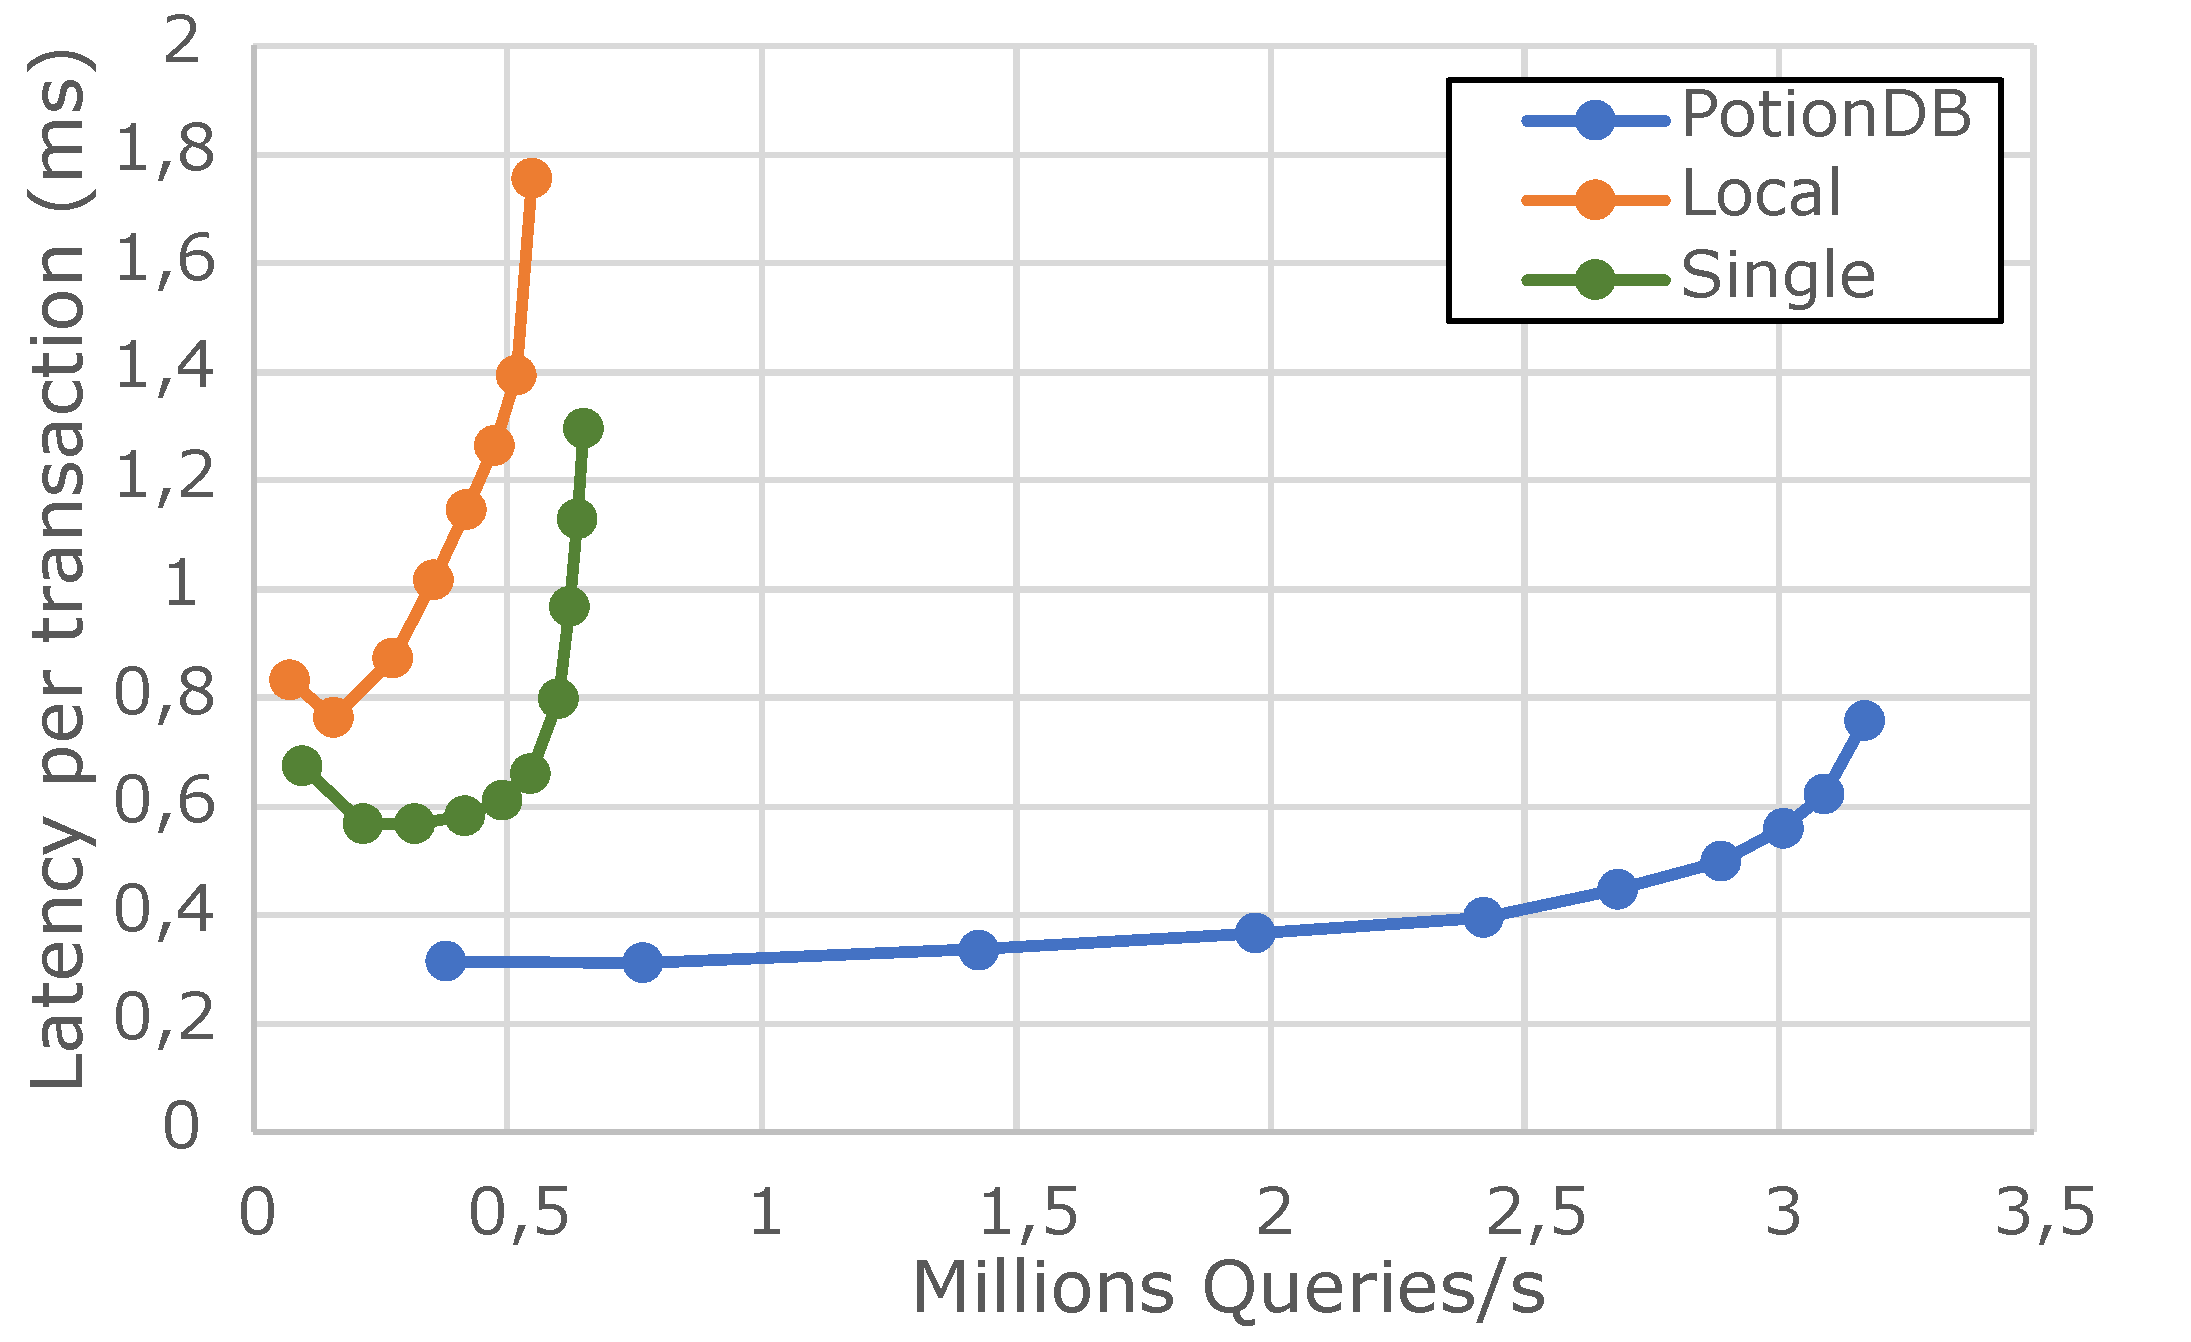
\includegraphics[width=.9\linewidth]{clientScale_cut}
		\caption{All queries}
		\label{fig:global_local_single}
	\end{subfigure}%
	\begin{subfigure}{.5\linewidth}
		\centering
		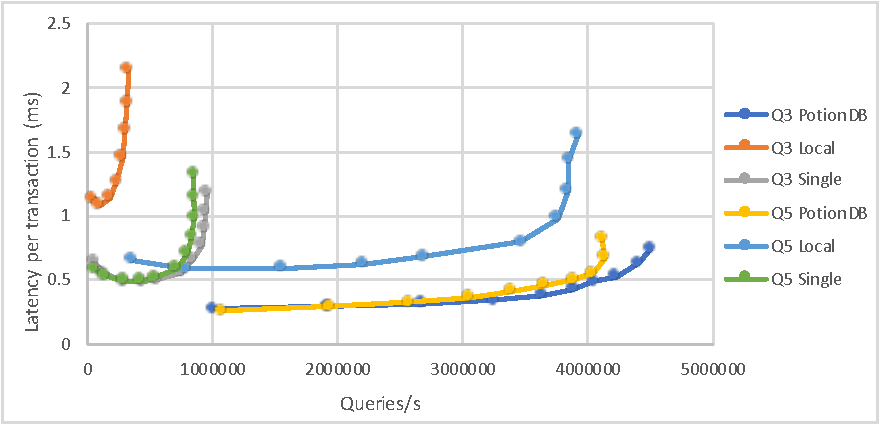
\includegraphics[width=.9\linewidth]{Q3vsQ5_cut}
		\caption{Single query type}
		\label{fig:q3q5}
	\end{subfigure}
	\caption{Query-only performance of PotionDB and its local and single view versions. On the left all queries are executed, while on the right only Q3 or Q5 are.}
	\label{fig:query_only}
\end{figure}

Figure \ref{fig:query_only} shows the results of experiments for the three versions of PotionDB, in terms of query/s versus latency.
Figure \ref{fig:global_local_single} includes all queries in the execution, while \ref{fig:q3q5} only includes a single type of query at a time.

When factoring in all queries (Figure \ref{fig:global_local_single}), as expected both local and single view PotionDB perform worse than (normal) PotionDB.
The single version's max throughput is about 1/5th of PotionDB's.
This occours due to queries being entirely served by views, which are all in a single server - thus, in a query-only scenario, one server gets all the load, instead of it being distributed across 5 servers.
The local version has about 1/6th of PotionDB's performance, as 2/3rd of the queries require data from all regions, which implies that in local mode such queries need to consult the views in every server.
The redirection of requests (see Section \ref{subsec:operationsNonLocal}) required to consult the views of others servers implies an extra round-trip for most queries. It also implies waiting for all servers to reply in order to complete a transaction, further reducing thoughput and increasing latency.

In Figure \ref{fig:q3q5} the focus is on two particular queries. Query 3 (Q3) requires data from all over the globe, while Query 5 (Q5) can be answered with data from a single region.
Thus, Q5 fits well both normal and local versions of PotionDB.
In fact, Q5's performance in local and normal modes is very similar - both reach a max throughput of around 4 million queries/s.
This occours as clients query data concerning the region of the server they are connected to, thus there is no need to contact other servers even in the local version.
As for the single version, Q5's performance is about 1/5th of the other two.
On the other hand, Q3 is a perfect example of how data locality affects performance.
This query requires data from all servers, thus in the local version every server needs to be contacted. The extra pressure on the servers (as all servers are required to answer all queries), as well as the extra round-trip, alongside bigger transfers of data, lead to a decreased performance of about 1/13th compared to PotionDB.
The single version has, as expected, about 1/5th of PotionDB's performance.

\begin{figure}
	\centering
	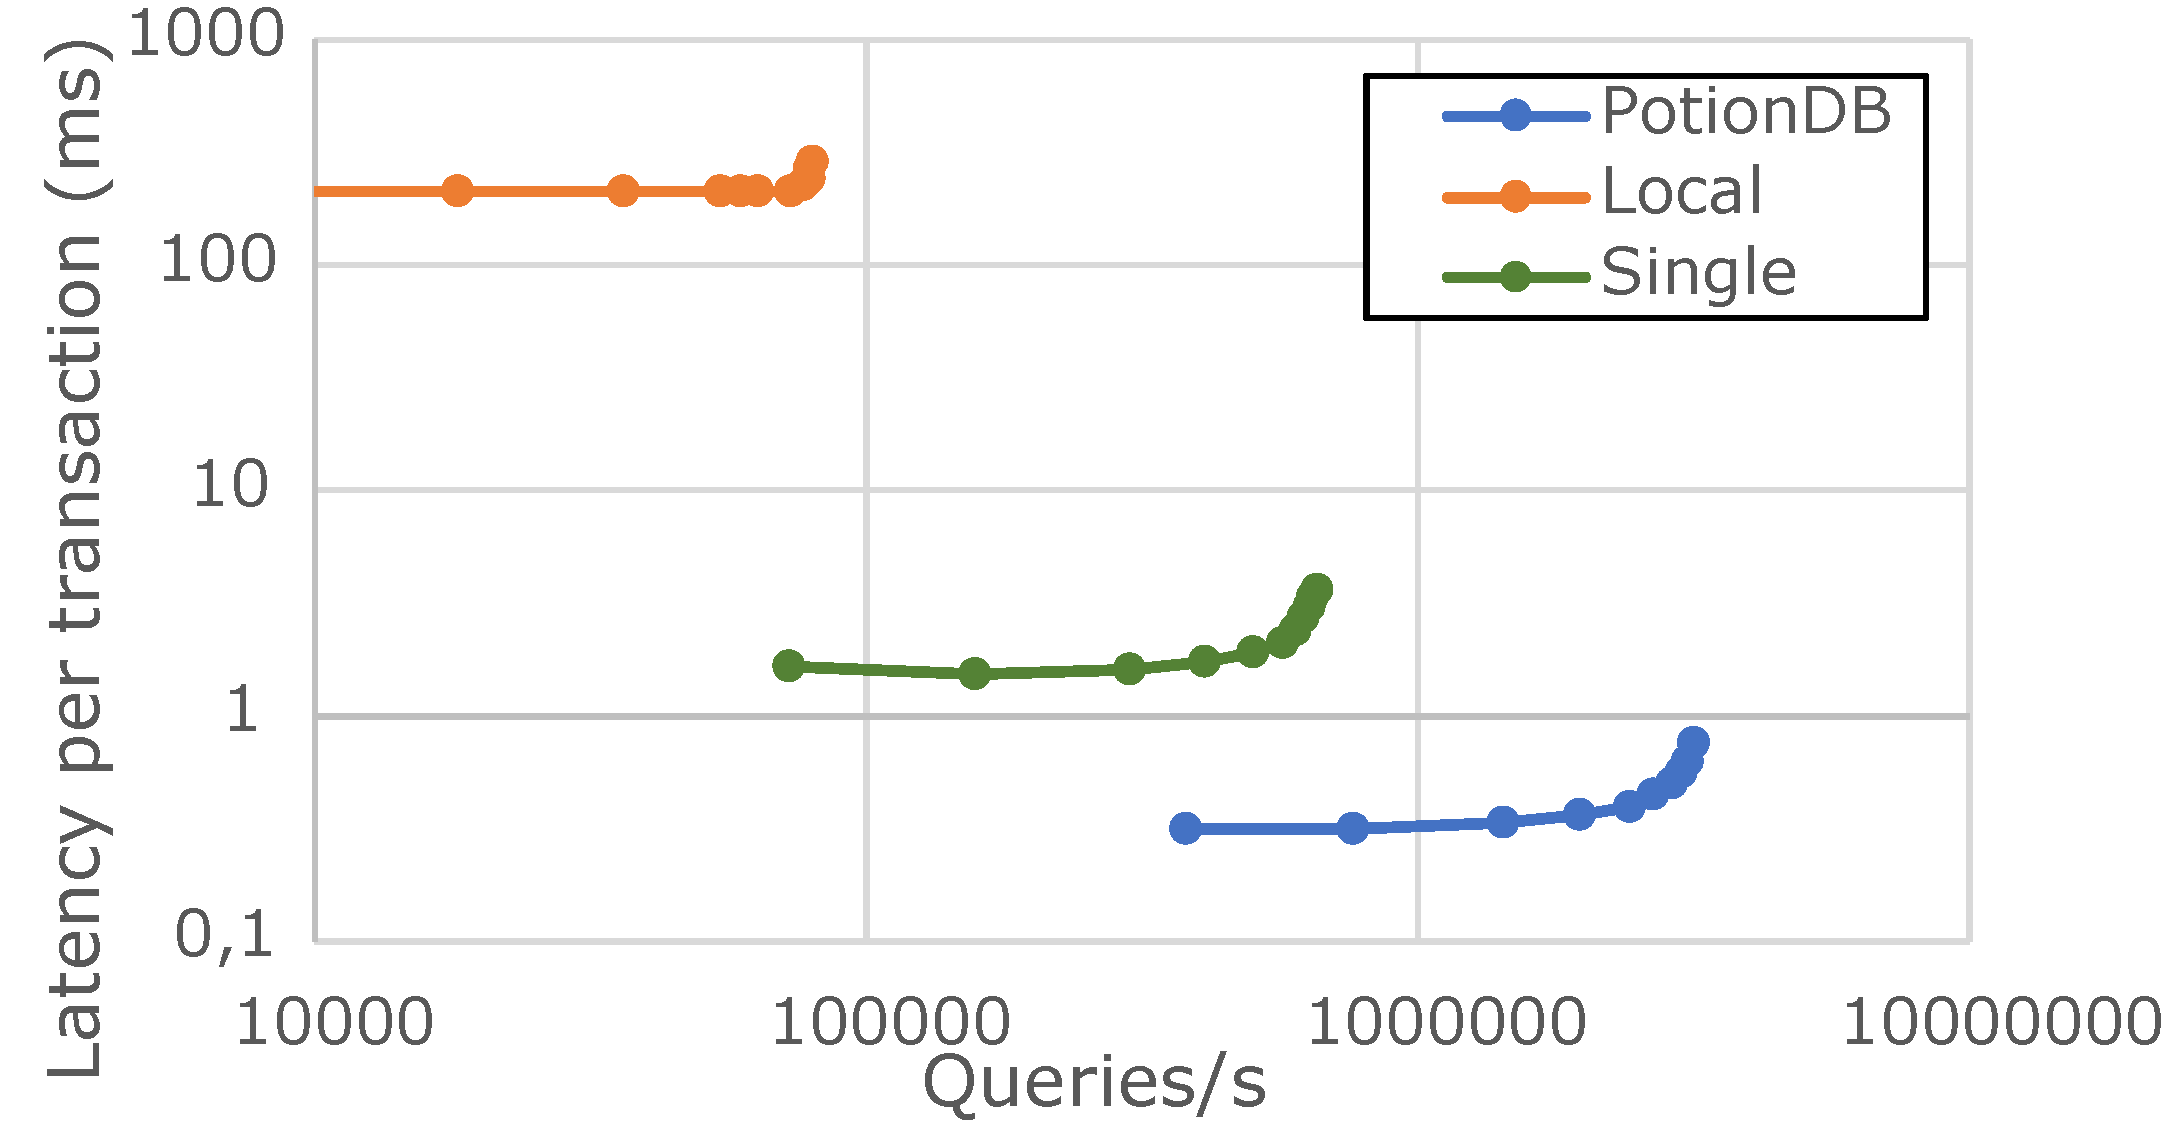
\includegraphics[width=.75\linewidth]{clientScale_tc_cut}
	\caption{PotionDB's performance executing all queries with added latency. Both axes have a log(10) scale.}
	\label{fig:global_local_single_tc}
\end{figure}

In the previous tests the latency of the clients to all servers is very low, as all servers and clients are connected in a LAN.
Figure \ref{fig:global_local_single_tc} shows the result of adding latency between servers (clients still retain low latency to represent being close to their server of choice).
Normal PotionDB is "unnafected" in terms of throughput and client's latency as clients only contact their nearby server - since no latency is added between client-server, no effect is noticeable.
In a scenario with updates however, an effect would be noticeable "under the hood" - replication would take longer to happen due to the imposed latency, thus a given client would take longer to be able to see the effects of updates executed on servers other than the one said client is connected to.
This would not affect query throughput, instead only the freshness of data.
For single PotionDB, a higher latency is noticeable compared to Figure \ref{fig:global_local_single}.
This happens as most clients will have high latency (i.e., the ones not connected to the server with the views) and do few operations, while the remaining ones will be operating directly on the view server.
The ones operating directly will be responsible for the majority of the load in the server with views - hence why the average client's latency increased midly.
As such, as long as more clients are used compared to Figure \ref{fig:global_local_single}, a similar max throughput is still achieved.
Finally, it is on local PotionDB where the effects of latency are most noticeable - here, for 2/3rd of the queries, all servers will be contacted. Since all transactions consist in one of each type of query, this implies all transactions will take, at least, as long as a RTT between the two most faraway servers - hence the observed latency of about 210ms.
Compared to Figure \ref{fig:global_local_single}, the max throughput is much lower. This is due to the much higher amount of clients needed to sature the servers: aproximately 3000 clients instead of 160.
The much higher amount of connections to each server, as well as the much more frequent "swap" of the processor cores between each client justify this lower throughput.

\subsubsection{PotionDB scaling - queries VS updates}

We now evaluate the impact on PotionDB's throughput of executing updates alongside queries, with multiple read/write ratios (\ref{enum:question2}).
In this scenario, when a client wants to execute an operation, it picks at random whenever a query or an update is executed.

In TPC-H an update is defined as the replacement of an old order with a new one.
As such, our granularity of update is the addition and removal of an order, with the associated items and necessary views' updates.
Finally, it is worth noting that even though some updates will execute in multiple replicas (e.g.: view updates), we only count one execution in our graphs.
%It is worth noting that an update affects both base data and all associated views.
%Also note that while view updates are executed in every replica, we only count them once (i.e., if one update is executed 5 times, it still only counts as 1 operation).

\begin{figure}
	\centering
	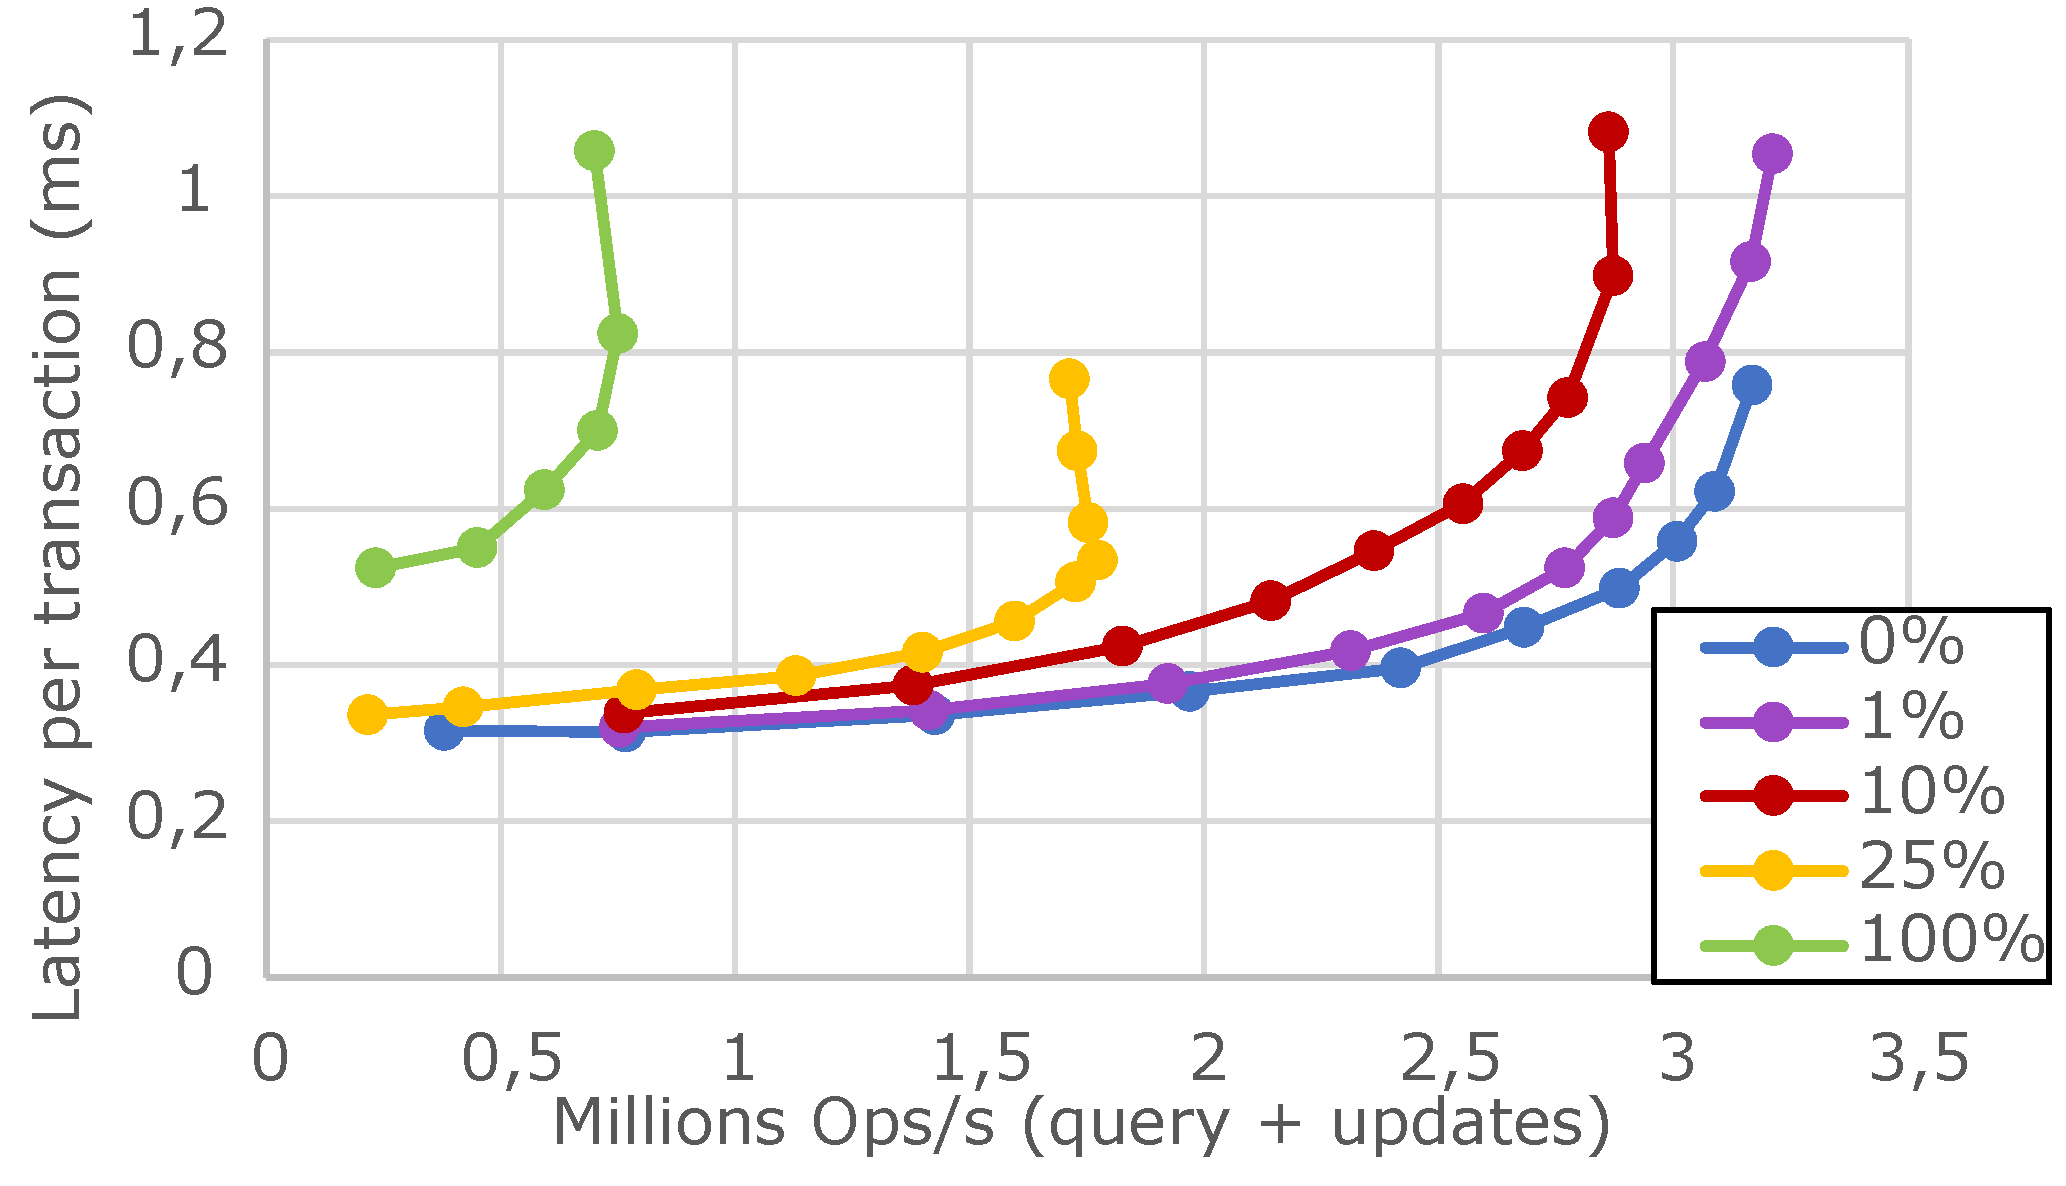
\includegraphics[width=.75\linewidth]{updRate_global_cut}
	\caption{PotionDB's performance with varying update rate.}
	\label{fig:update_rates}
\end{figure}
\begin{figure}
	\centering
	\begin{subfigure}{.5\linewidth}
		\centering
		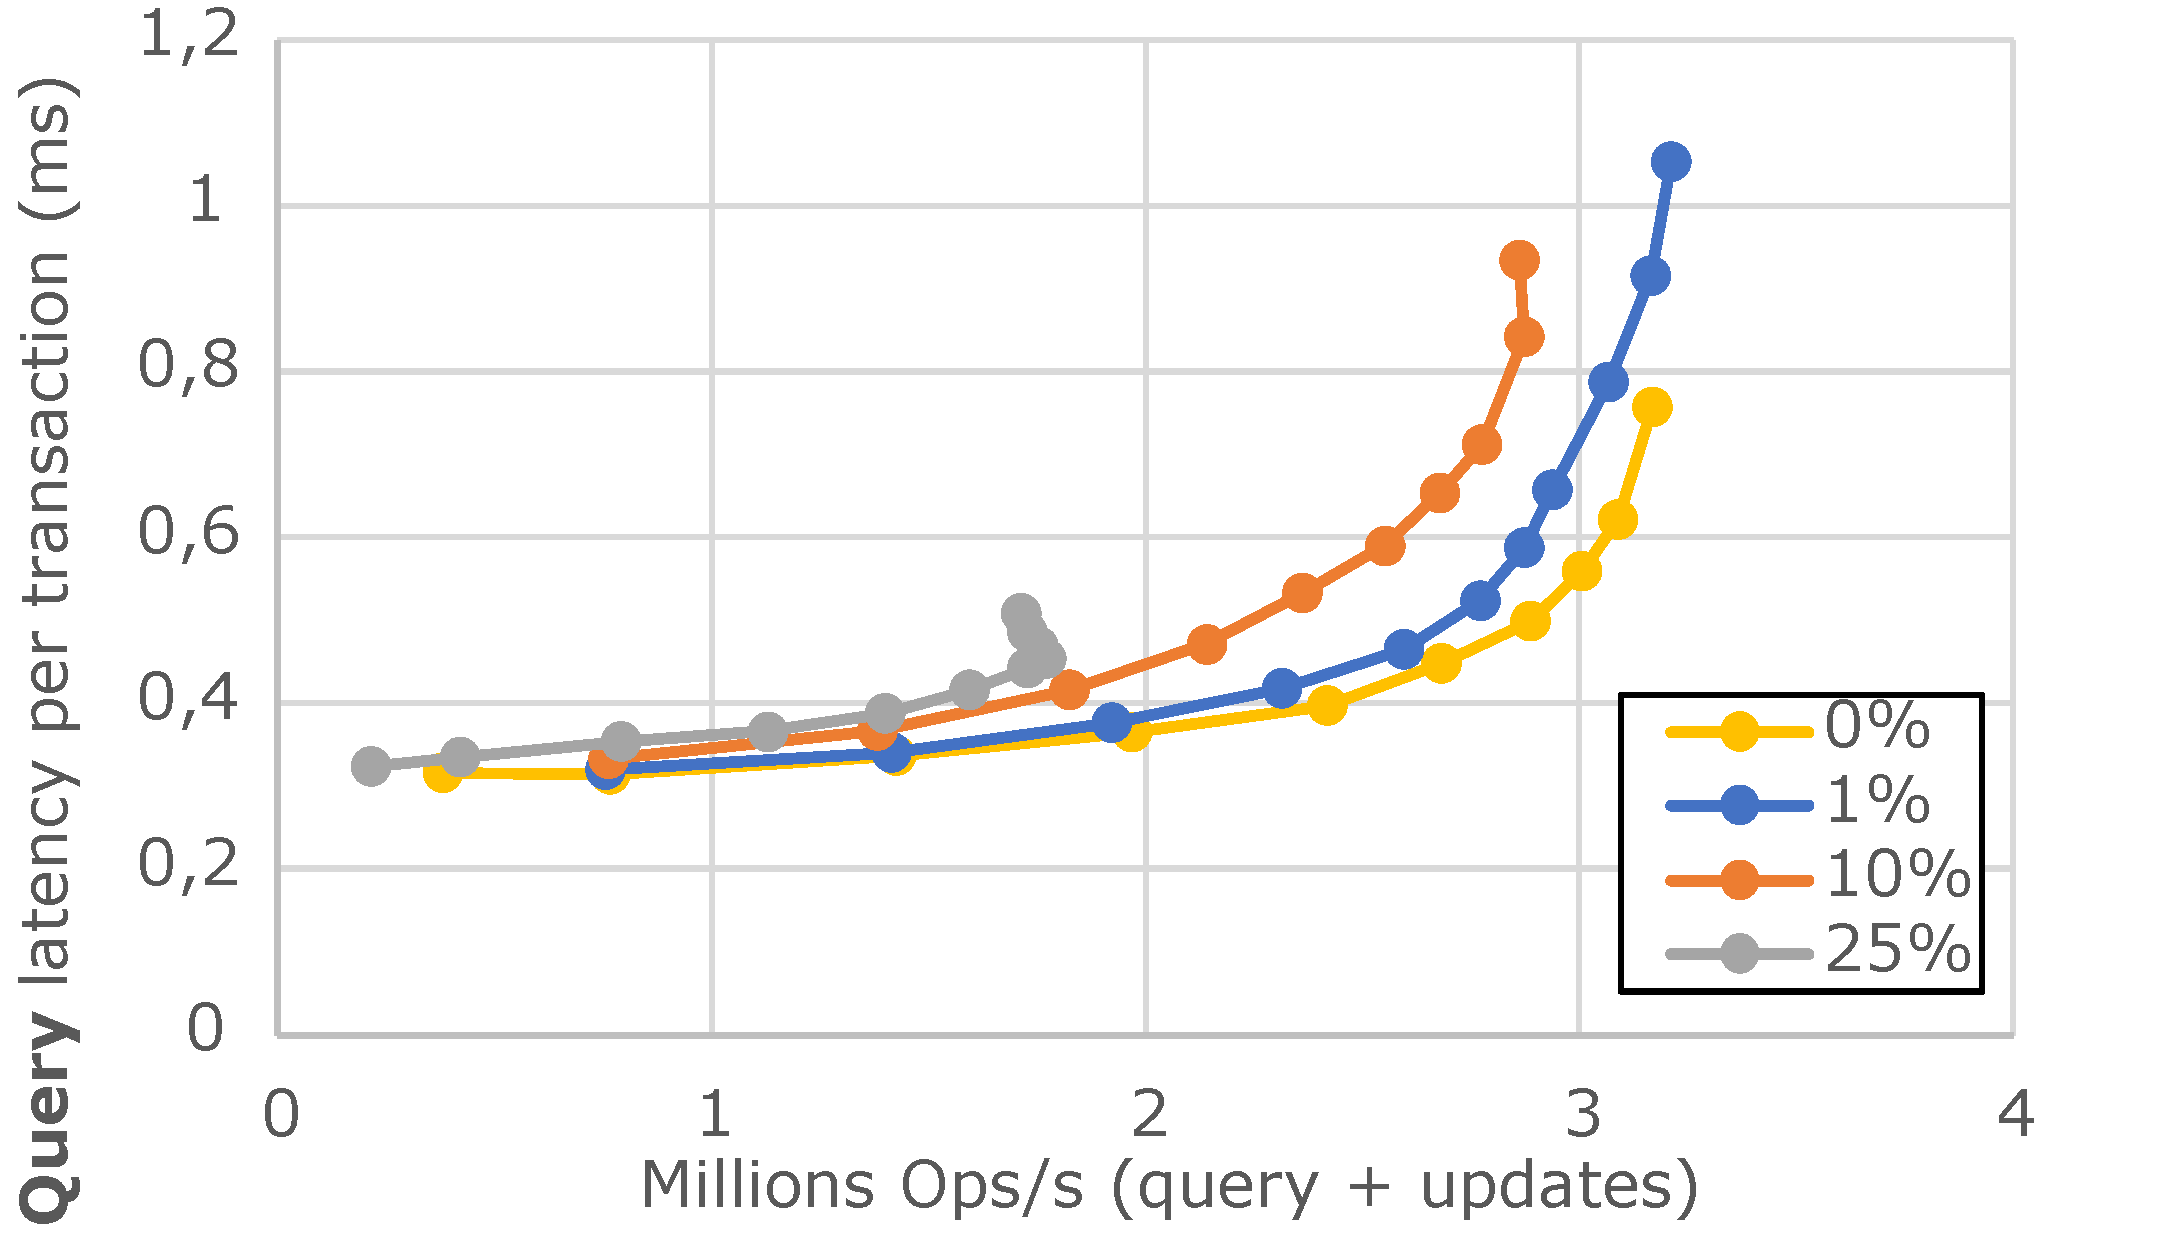
\includegraphics[width=.99\linewidth]{updRate_queryLatency_cut}
		\caption{Query-latency}
		\label{fig:update_rates_query}
	\end{subfigure}%
	\begin{subfigure}{.5\linewidth}
		\centering
		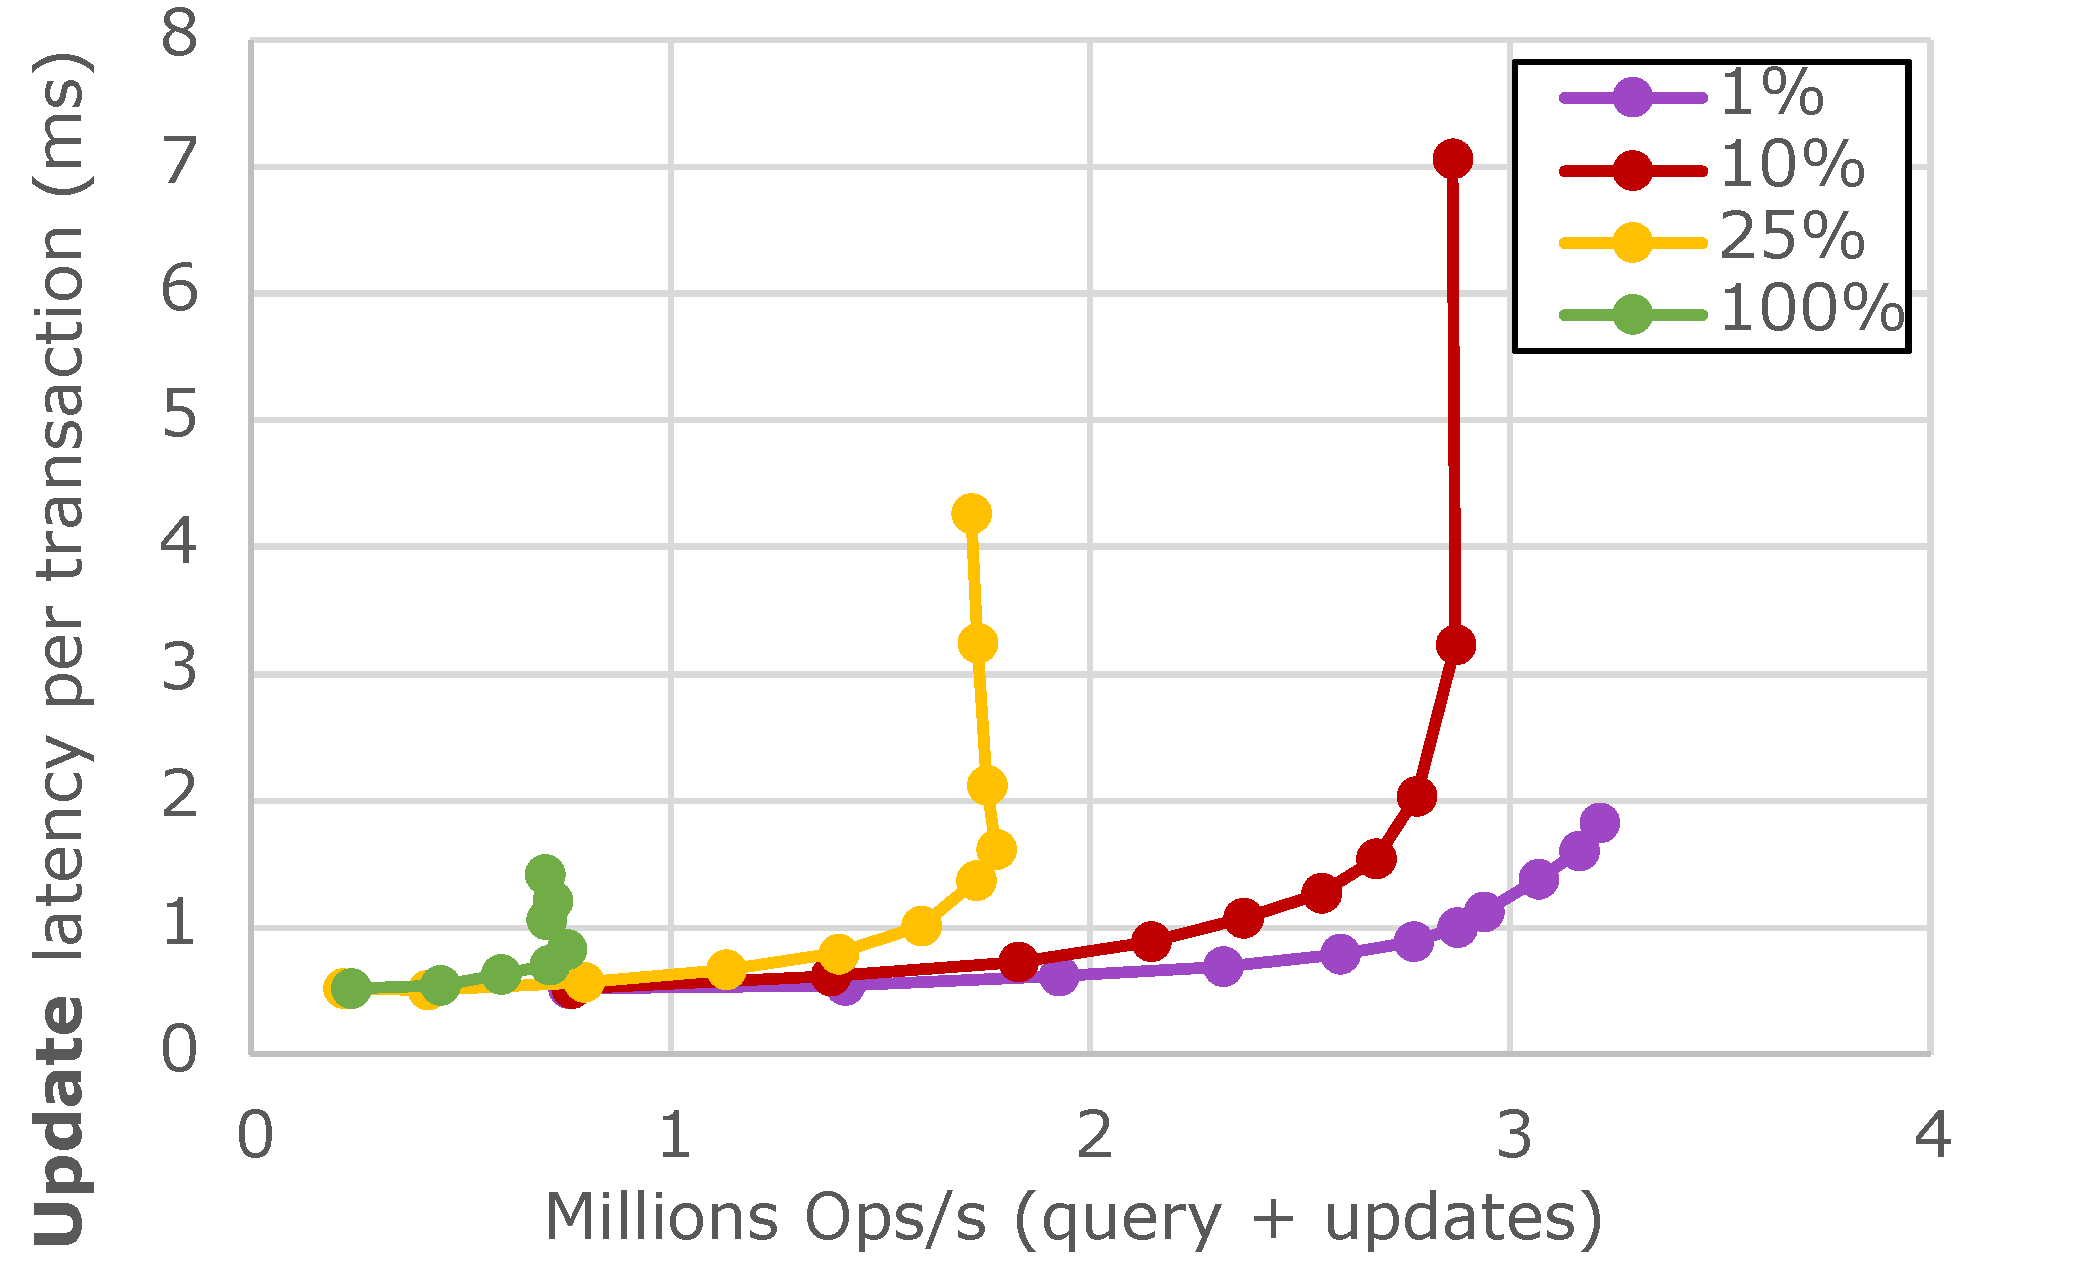
\includegraphics[width=.99\linewidth]{updRate_updateLatency_cut}
		\caption{Update-latency}
		\label{fig:update_rates_update}
	\end{subfigure}
	\caption{PotionDB's performance with varying update rate, with query and update latencies split. Note that each update transaction adds and removes one order, as well as associated items and views, thus having more operations than one query-only transaction.}
	\label{fig:update_rates_split}
\end{figure}

Figure \ref{fig:update_rates} shows the results of executing updates alongside queries, with varying odds of choosing an update.
For low update rates (1\% and 10\%), the decrease in performance can be considered reasonable: aproximately 4\% and 16\%.
For higher rates, two observations can be made:
\begin{enumerate*}[label=(\roman*)]
	\item the servers saturate earlier, in some cases even decreasing throughput as the number of clients rises;
	\item the max throughput is lower.
\end{enumerate*}

The referred observations can be explained by considering the following. 
With PotionDB's sharding (Section \ref{subsec:sharding}), queries on objects of different shards can be executed concurrently, thus query-only scenarios scale easily. 
However, transactions with updates must lock the partitions they are involved and do our commit protocol in order to ensure the states evolve sequentially in a replica even when concurrent transactions are issued.
As such, if the update rate is high, clients executing queries or updates may often have to wait for a transaction with updates to finish executing before executing their own operations.

Figure \ref{fig:update_rates_split} shows the same experiment as Figure \ref{fig:update_rates}, but showcases the latencies of queries and updates splitted, instead of together.
It is noticeable that updates, even with few clients, have higher latency than queries - this is mostly due to update transactions having more operations than queries.
The abrupt spike observed at the end in the update latency graph happens as many clients are doing updates and, thus, many commits with locks are issued, which have to wait for each other to finish.

\begin{figure}
	\centering
	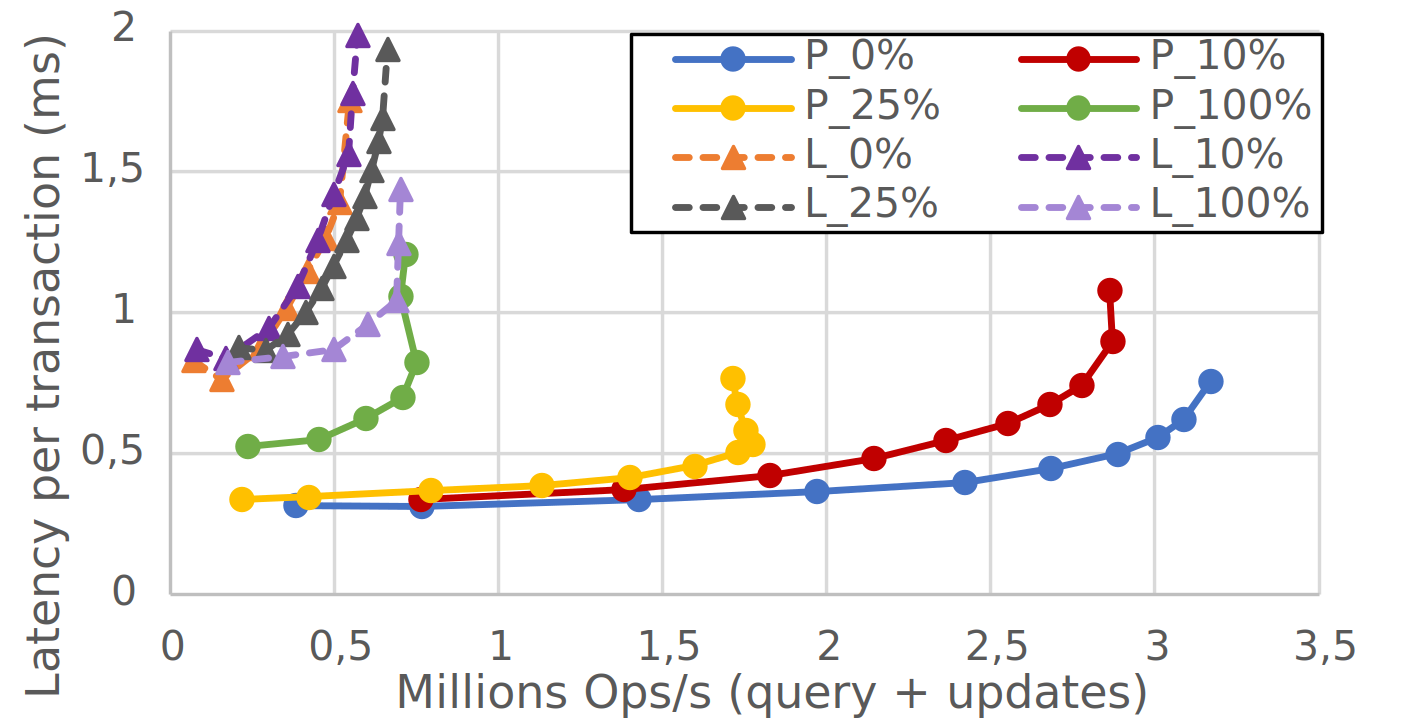
\includegraphics[width=.7\linewidth]{updRate_localvsglobal_cut}
	\caption{Normal(P\_) and Local (L\_) PotionDB's performance with varying update rate.}
	\label{fig:update_rates_normal_vs_local}
\end{figure}

\andre{Note: I'm not sure on the explanation below. Basically, in local mode, more update ops are done per transaction, thus actually less orders are updated in the same period of time. However, since views are local, there's less replication work. Not much redirection is done as 50\% of the orders are fully local, and most others have few regions.}

Figure \ref{fig:update_rates_normal_vs_local} showcases the performance of both PotionDB and local PotionDB with varying update rates.
As expected, local PotionDB performs worse than PotionDB.
However, as the percentage of updates increases in local PotionDB, so does the throughput.
This happens as updates are not as hindered by views being split per region as queries.
Aproximately half of the orders are local to a region \footnote{This does not occour on the original TPC-H dataset, whose items of orders are totally random. We did this modification to add locality to orders. This helps local PotionDB more than PotionDB.} while most others refer few regions, thus not many view updates need to be redirected to other servers.
Besides, since each view only contains local data, updates to a view do not need to be replicated to every other server, reducing the load on the servers due to replication.
These factors added up allow local PotionDB to have higher performance when updates are added and end up with a similar throughput to PotionDB when only updates are executed.

\andre{Maybe a graph of local VS normal PotionDB with updates of all views and only queries of Q5? That query has high performance in both modes - may be interesting to see how it scales with updates (I wonder if local PotionDB has higher throughput than normal in that scenario?)}

We now consider a scenario with latency added between servers, as described in Section \ref{subsubsec:commonSettings}.
Recall that on normal PotionDB, as previously discussed, throughput isn't affected as clients only interact with the server they are close to, even when doing updates.
They would, however, take longer to see the effects of updates done on views that were executed in other servers, due to the added latency on replication.

\begin{figure}
	\centering
	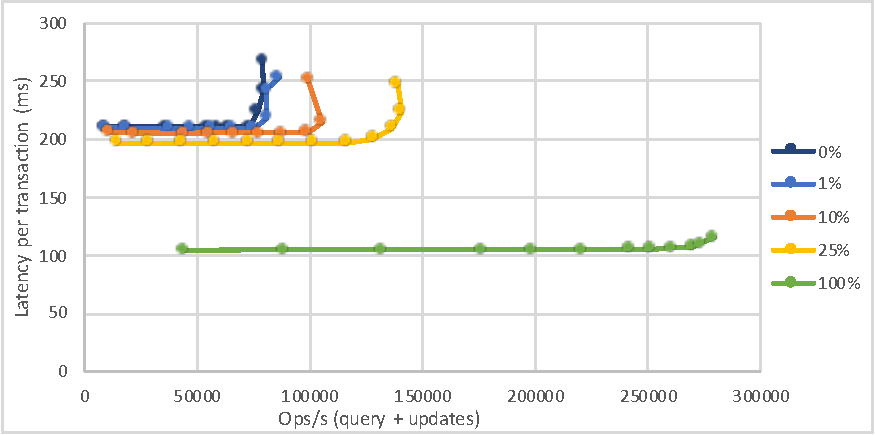
\includegraphics[width=.7\linewidth]{updRate_tc_cut}
	\caption{Local PotionDB's performance with varying update rate, with latency added.}
	\label{fig:update_rates_tc}
\end{figure}

Thus, we focus on local PotionDB, which is shown on Figure \ref{fig:update_rates_tc}.
We can easily observe that as the percentage of updates rise, the maximum throughput also rises quickly.
At a first glance this may seem confusing, however the following justifies this behavior:
\begin{compactitem}
	\item Updates have lower latency than queries, as each update transaction only needs to contact a subset of servers, unlike query transactions which need to contact all. Thus, they can often avoid the connection with highest latency.
	\item Updates have more operations per transaction than queries, which means more operations done per round trip.
\end{compactitem}

\andre{Should I mention that a lot less clients are needed to sature the server, the higher the update rate is? (mainly on scenarios without latency)}
\andre{Probably some concluding note that reffers that for PotionDB's intented usages it is likely that updates are much less frequent than queries, or maybe even that updates could maybe be delayed?}

\subsubsection{CRDT Benchmarks}

%\andre{Note: On the graphs here I forgot to put "Latency per transaction (ms)" instead of just "Latency (ms)"... will fix that when we do a final version of those graphs}

We now focus on evaluating the performance of the CRDTs used to build the views of TPC-H.
Namely, we test TopK, TopSum, Counter and Average CRDTs.
\andre{TODO: Maybe I should test embedded maps too? Since they are used to ``hold'' multiple CRDTs in Q5, acting as a group by.}

In this scenario, we drop the TPC-H dataset.
Instead, for each test we prepare 20 CRDTs with random initial data (the same amount of CRDTs used for Q15’s views, discussed in Section \ref{subsec:implementedQueries}).
%Instead, we prepare each CRDT with some random initial data.
%In each test, 20 CRDTs are created/manipulated by the clients (the same number of CRDTs that are used to build the views for Query 15, discussed in Section \ref{subsec:implementedQueries}).
Each client picks a CRDT randomly following an uniform distribution and uses said CRDT to do query and/or update operations. 
%Then, each client does query and/or update operations on one of the CRDTs.
The number of operations per transaction is the same as in the TPC-H scenario. \andre{(Do I need to define this in the TPC-H scenario?)}
%The distribution of CRDTs is the type "shared"


%TOPK test max throughputs: 11.3M, 10.3M, 3.1M, 0.37M
\begin{figure}
	\centering
	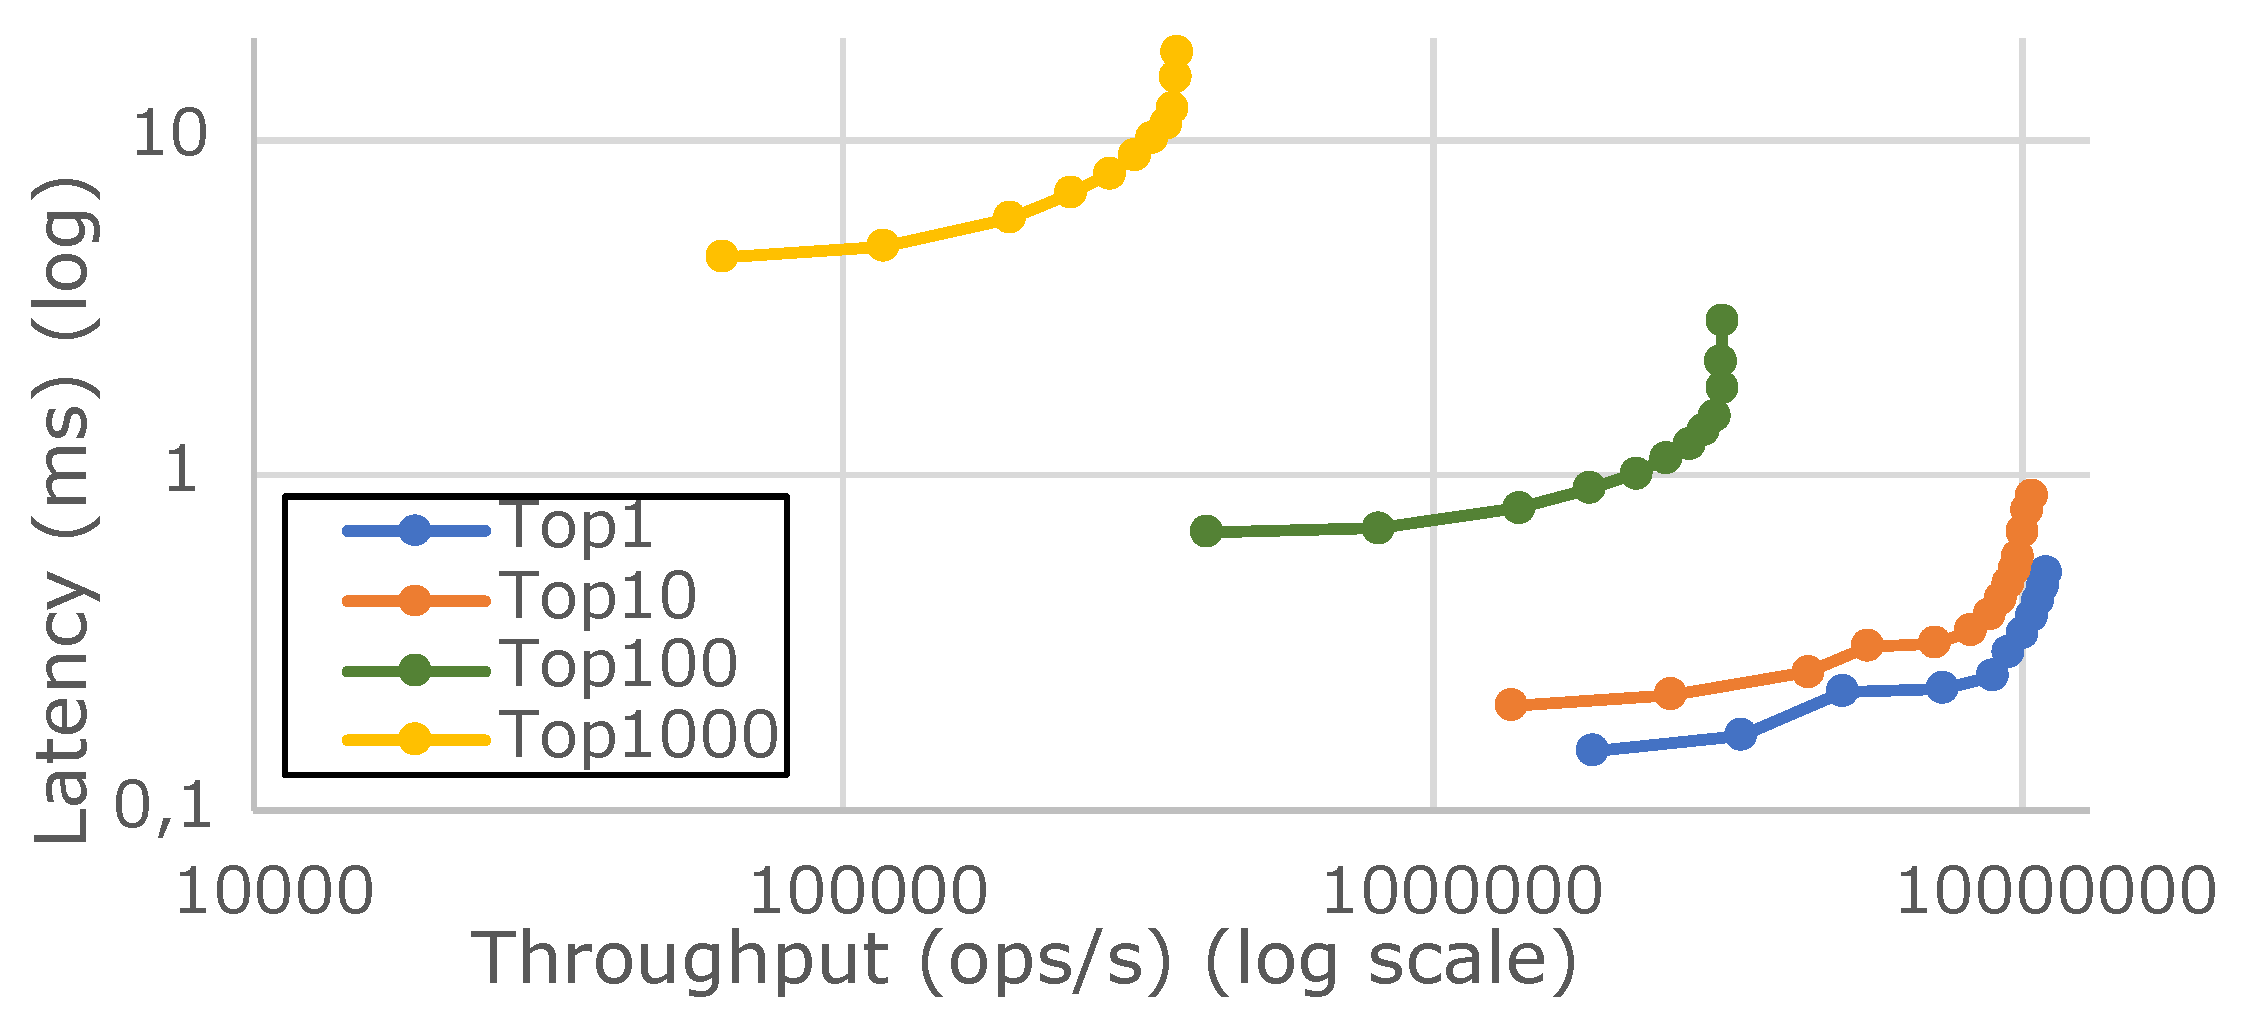
\includegraphics[width=.7\linewidth]{TopKTopSize0upd_cut}
	\caption{TopK query performance with a varying top size.}
	\label{fig:TopkSize0upd}
\end{figure}

Figure \ref{fig:TopkSize0upd} contains the results of executing TopK queries with different values for K.
The throughput difference between Top-1 and Top-10 is small (10\%). This happens as the amount of data transfered is small compared to the communication overhead (latency + metadata transfered, alongside the cost of serializing/parsing the protobufs for request and reply), as well as the overhead of handling a high amount of clients.
As the size of the TopK increases, the query performance drops as the amount of data transfered starts to become more relevant.
From Top-10 to Top-100 and Top-100 to Top-1000 the throughput decreases by, respectively, 70\% and 88\%.
We expect that after 1000, increasing linearly the number of elements on top will decrease the throughput by the same factor.
%\andre{Should I mention throughput numbers? The max of each is 11.3M, 10.3M, 3.1M, 0.37M ops/s.}
%\andre{Is it relevant to mention the number of entries in the TopK? (10000, same as in Q15) If so, how/where do I mention that?}

\begin{figure}
	\centering
	\begin{subfigure}{.5\linewidth}
		\centering
		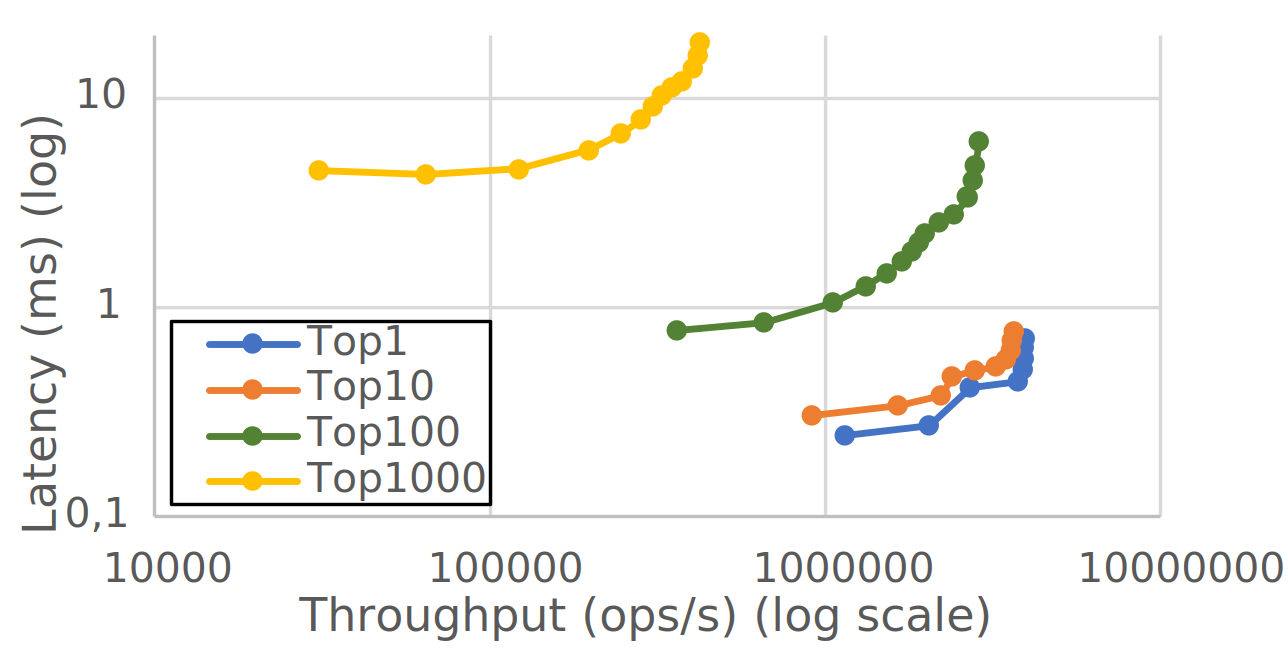
\includegraphics[width=.97\linewidth]{TopKTopSize25upd_cut}
		\caption{TopK with 25\% updates}
		\label{fig:TopkSize25upd}
	\end{subfigure}%
	\begin{subfigure}{.5\linewidth}
		\centering
		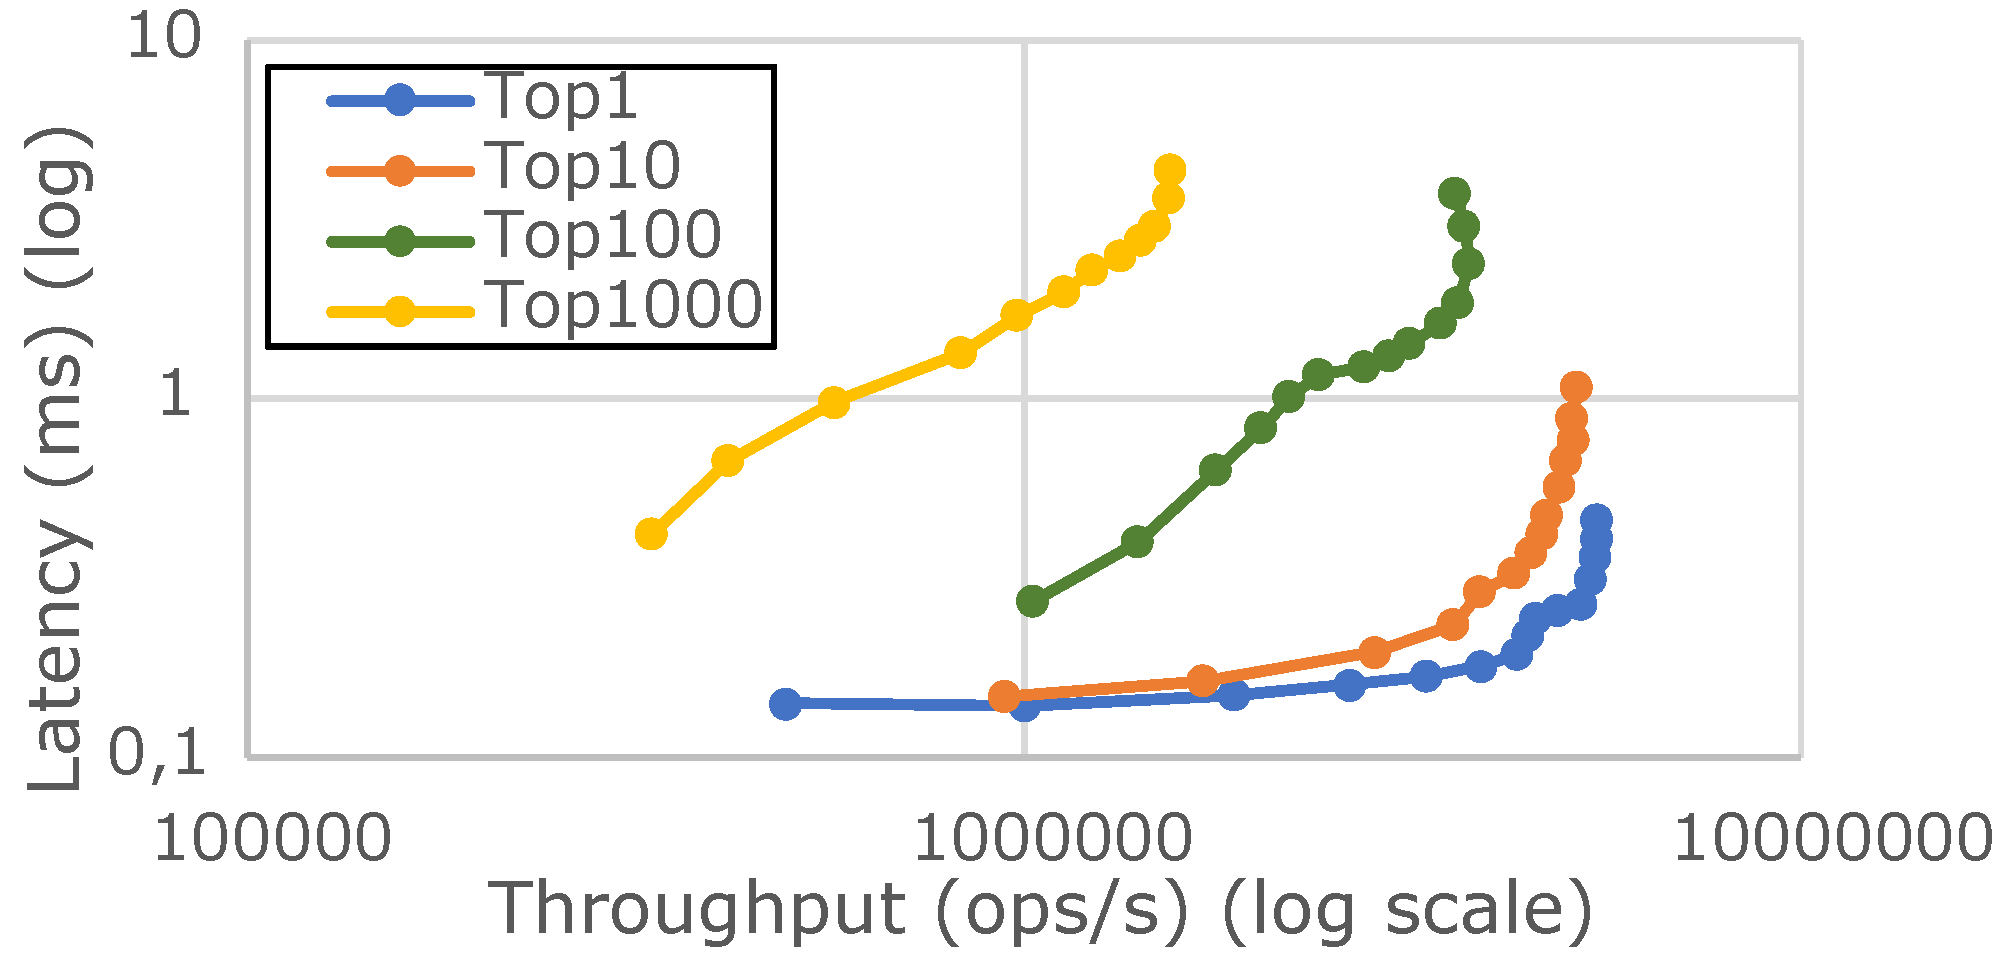
\includegraphics[width=.97\linewidth]{TopKTopSize100upd_cut}
		\caption{TopK with 100\% updates}
		\label{fig:TopkSize100upd}
	\end{subfigure}
	\caption{TopK operations (query + update) performance with varying top size.}
	\label{fig:TopkSize25_100upd}
\end{figure}


Figure \ref{fig:TopkSize25_100upd} contains the same test as before but with, respectively, 25\% and 100\% updates.
The differences in performance here are different compared to query-only's scenario.
This happens as on updates, the amount of data transfered is similar for all scenarios. 
However, as expected, as the value of K increases, adding or removing elements to the top gets more expensive.
\andre{Not sure if/how I explain this. I believe the reason why it becomes more expensive is because of when the TopK needs to search for the ``new minimum'' of the top - since the elements ``not in top'' are stored as a set, sometimes that entire set needs to be searched upon to find a new minimum.}

%\andre{Note: Interestingly, the TopSum graphs for 100\% updates are quite different from TopK. TopSum scores 5M ops/s on all top sizes for 100\% updates (to be precise: 5.4M, 5.4M, 5.3M, 5.1M Top1, Top10, Top100, Top1000); while TopK scores below 2M ops/s for Top1000. I haven't searched yet why it is like that.}

\begin{figure}
	\centering
	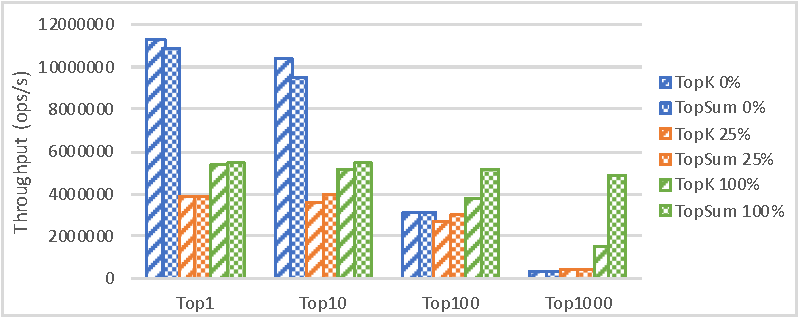
\includegraphics[width=.7\linewidth]{TopKVSTopSum_cut}
	\caption{TopK and TopSum performances for different top sizes and update rates.}
	\label{fig:TopkVSTopsum}
\end{figure}

Figure \ref{fig:TopkVSTopsum} shows how the TopSum compares to the TopK CRDT in similar scenarios.
When only executing queries, the performance is very similar. 
However for high update rates, TopSum handles updates better than TopK.
\andre{TODO: I have to check why this is happening... some guesses: 1- TopSum doesn't have removes but rather incs/subs, so less elements being removed/created from each set (but still, some should when moved between top and not-top) ; 2 - topK has tombstones, topSum does not (but should be okay as it is only 1 timestamp per element) ; 3 - TopSum uses pointers to structures for the elements while TopK uses structures ; 4 - some other reason? Like different behaviour? I don't know. Maybe I need to test with a Map or Set CRDT. But even so it is odd...}

\begin{figure}
	\centering
	\begin{subfigure}{.33\linewidth}
		\centering
		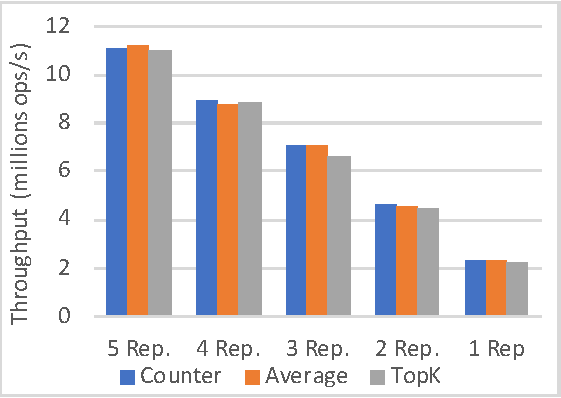
\includegraphics[width=.97\linewidth]{CounterAvgTopK0upd_v2_cut}
		\caption{0\% update rate}
		\label{fig:CounterAvgTopK0upd}
	\end{subfigure}%
	\begin{subfigure}{.33\linewidth}
		\centering
		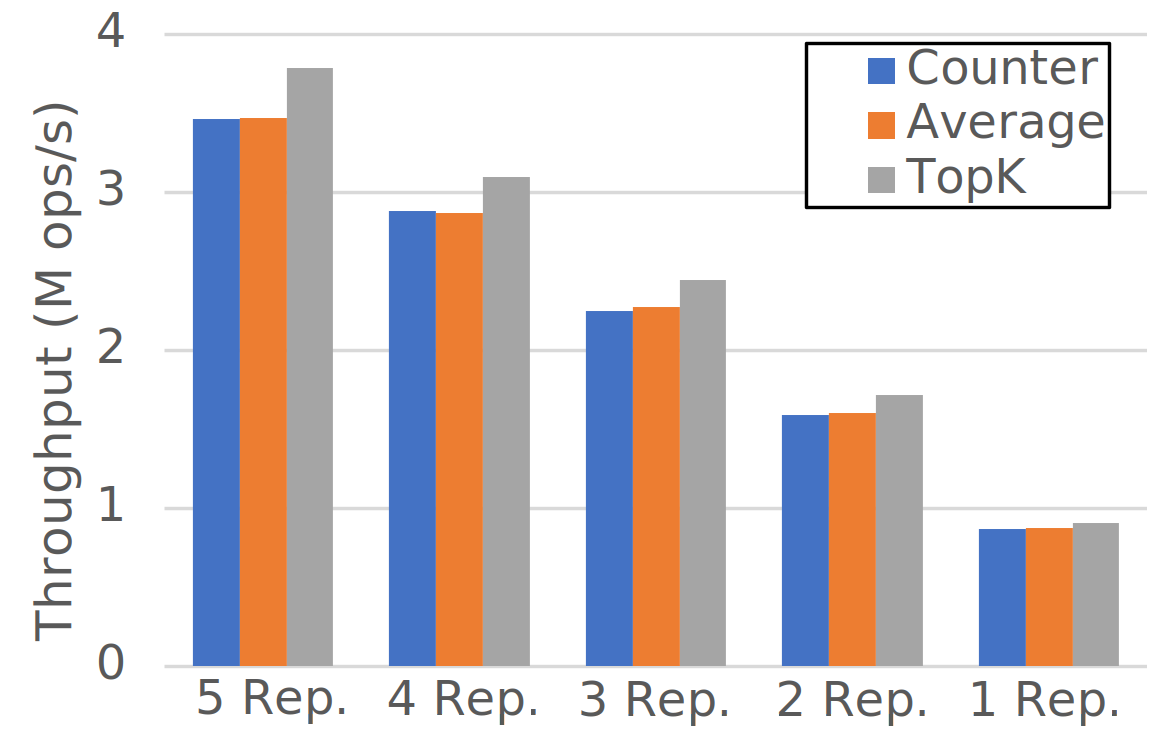
\includegraphics[width=.97\linewidth]{CounterAvgTopK25upd_v2_cut}
		\caption{25\% update rate}
		\label{fig:CounterAvgTopK25upd}
	\end{subfigure}%
	\begin{subfigure}{.33\linewidth}
		\centering
		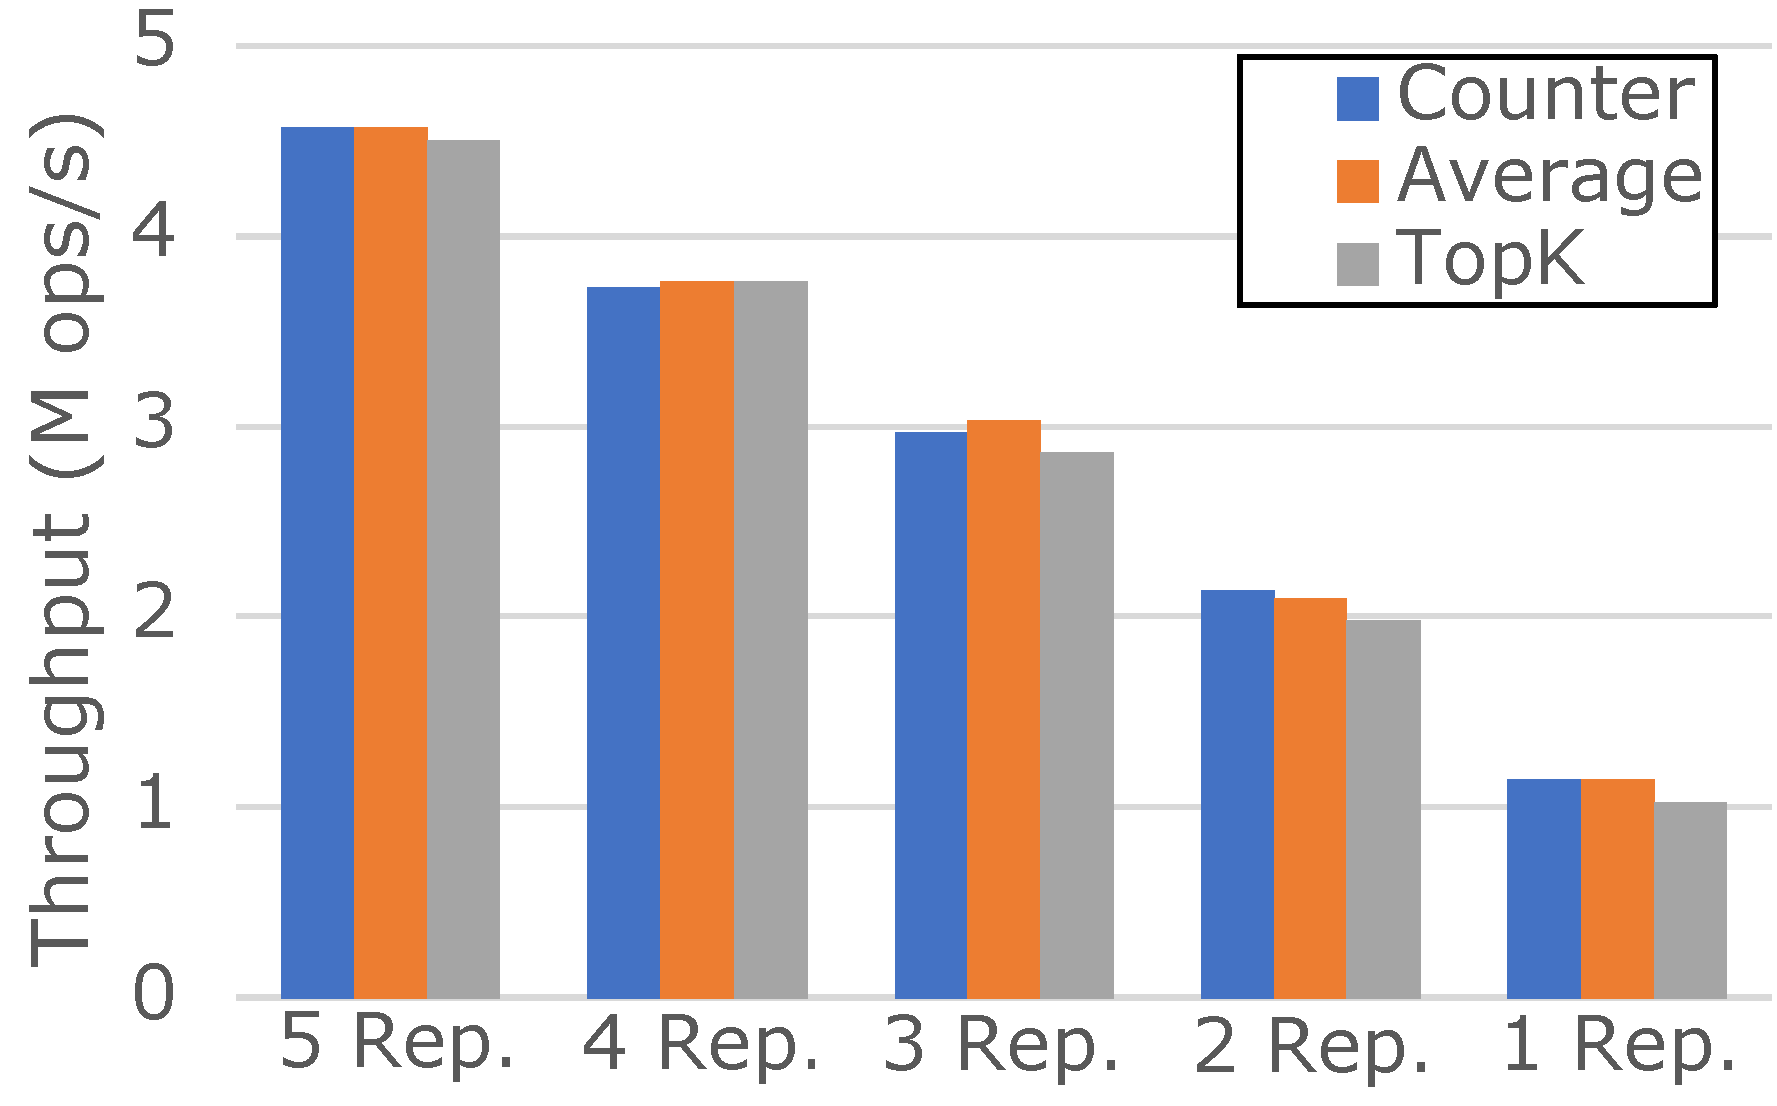
\includegraphics[width=.97\linewidth]{CounterAvgTopK100upd_v2_cut}
		\caption{100\% update rate}
		\label{fig:CounterAvgTopK100upd}
	\end{subfigure}
	\caption{Counter, Average and TopK CRDTs performance for different numbers of replicas and update rates.}
	\label{fig:CounterAvgTopK}
\end{figure}

Figure \ref{fig:CounterAvgTopK} shows the max throughput of Counter, Average, and TopK (top of one) CRDTs.
In these tests we try to assess how the performance of CRDTs scales with the number of replicas.
When executing queries-only, the performance scales aproximately linearly with the number of servers for the three CRDTs, with all three CRDTs having similar throughput.
For instance, Average CRDT goes from 11.1M ops/s with 5 servers to 2.35M ops/s with 1 server (78.8\% decrease).
This happens as any server can be queried without needing to synchronize with other servers.
With updates, the max throughput is lower and it scales down less linearly.
For example, Average CRDT with 25\% update rate goes from 3.46M ops/s with 5 servers to 2.87M ops/s with 4 servers (17.1\% decrease) and to 1.11M ops/s with 1 server (67.9\% decrease from 5 servers).
A similar percentage drop is observed with 100\% updates.
This happens as updates have to be propagated and executed in every other replica.
However, PotionDB's replication mechanism groups updates from different transactions, allowing them to be executed more efficiently.
\andre{No idea why topK has a bit more performance with 25\% updates. I'm not sure why update-only has better throughput than query+update, but I can think of two possible reasons: a) updates make queries wait; b) updates reply quicker as a reply is sent as soon as the partitions confirm they will commit (and not after the commit is executed), unlike queries which must wait for the result to be ready.}

\section{Related Work}
\label{sec:related_work}

%TODO: Veronica uses projection to improve queries, might be worth comparing to.

Database systems can offer different levels of consistency, with solutions usually being labeled as either strong consistency or weak consistency.
Strong consistency systems \cite{spanner, slog, scatter, krikellas2010strongly, redblue, megastore} are easier to work with as they provide a total order for their transactions.
However, the CAP theorem \cite{cap} implies that availability may be compromised in case of network partitions.
Furthermore, high latency is to be expected in geo-distributed scenarios as multiple data centers must be contacted for commiting a transaction.
By relaxing the provided consistency guarantees, weak consistency systems \cite{dynamo, couchDB, cassandra, chainreaction, cops, riak, eiger} can provide low latency, high throughput and better fault tolerance.
However, concurrency conflicts make those solutions harder to work with.
Causal consistency is a sub-form of weak consistency that alleviates this problem, however anomalities can still be observed even with cross-object causality \cite{cops, burckhardt2013understanding}.

Both indexes and materialized views can speed up the execution of queries.
Indexes can provide quick access to a table or object using a non-primary key, and are often used by queries which require sorting or a given range of values.
Multiple systems implement indexes \cite{dynamo, couchDB, cassandra, megastore} and research on efficient usage and storage of those is a common research topic \cite{lee2020asymmetric, lisa, alex, bindex, slik}.
On the other hand, materialized views work as a cache for the result of a large query.
Materialized views can provide quick access to data that would take a long time to calculate, and are often useful for analytic queries \cite{analyticdb}.
\andre{[I didn't find a proper reference for ``views being useful for analytic queries''. Suggestions?]}
However, maintaining views consistent and automatically updated is challenging \cite{oracleViews, chronocache, birds} and few systems implement them \cite{chronocache, marviq, estocada, couchDB, oracleViews, noria}, even though they can speed up queries considerably.
To the best of our knowledge, PotionDB is the first system to support materialized views of global data in a partially geo-replicated scenario.

Geo-distributed scenarios imply high latency when acessing far away data centers, which is required for strong consistency \cite{chronocache, slog, cops, eiger}. 
Network partitions are also a concern, as they may render strongly consistent systems unavailable.
Weak consistency can help avoid both problems but lacks the useful consistency guarantees provided by strong consistency.

%\andre{I still need to find citations for partial replication. Any suggestion/starting point is more than welcome}

Partial replication allows to reduce storage costs and can potencially improve a system's performance, e.g., due to less operations being applied on each server \cite{sipre, optimisticPartial, coda}, and are thus of interest for geo distribution.
The partitioning of data must be carefully done by considering where each object is relevant, as otherwise clients may need to access far away servers and thus experience high latency \cite{sipre, optimisticPartial, coda}.
However, one common problem with partial replication is that, sometimes, it is necessary to query data sharded among different data centers \cite{sipre}.
%Many systems provide partial replication \cite{???}.
%However, a problem not often analyzed in these kind of systems is that some analytic queries may need to consult objects sharded between different data centers.
Without views, this process can be slow, specially when trying to provide a consistent snapshot of the database.
PotionDB tackles this problem by providing views that summarize partially replicated data and directly answer such queries.

Conflict-free Replicated Data Types, CRDTs \cite{crdt}, are replicated data types that guarantee state convergence as long as all updates are eventually delivered.
Thus, they are often used in weakly consistent systems, e.g., Redis \cite{redisCRDT} and Riak \cite{riak}.
Some types of CRDTs have been introduced that can help with representing views of data, namely computational CRDTs \cite{computationalCrdt} and non-uniform CRDTs \cite{Cabrita17Nonuniform}.
The former computes some result over data (e.g., a sum), while the later focus on minimizing the information that needs to be replicated to correctly reply to queries (e.g.: a top-k CRDT does not need all entries to be replicated).
In PotionDB every object is a CRDT and, in particular, we leverage on both computational and non-uniform CRDTs to support our views.

\andre{I did not really organize/compact the comparisons to other systems. Are they OK like this? Suggestions/changes are appreciated.}

ChronoCache \cite{chronocache} is a middleware caching layer for geo-replicated databases which focus on combining multiple queries into one request and caching query results.
While the caching can speed up future requests, complex queries may still need to contact multiple servers and updates can invalidade the cache or else clients read stale data.

AnalyticDB \cite{analyticdb} focus on optimizing analytic queries. 
It separates write and read paths to prevent complex queries from slowing down writes. 
It also makes usage of indexes to speed up queries.
However, complex queries still take hundreds of milliseconds to execute and may slow down other simpler queries.
They do not make usage of views.

SLOG \cite{slog} provides ACID transactions in a geo-replicated scenario.
They share one of PotionDB's insights - not all data is relevant everywhere and clients will often access data relevant in their region.
Thus, SLOG achieves low latency ACID transactions for transactions that can be served by a single data center.
However, unlike PotionDB, queries regarding data partitioned across multiple data centers has considerably higher latency.
We leverage on views of global data to prevent this.

ESTOCADA \cite{estocada} is a system designed to work with polystores and focus on taking advantage of each database's stronger points and make extensive usage of the materialized views provided on each.

%Preciso de rever este melhor (local/remoto?)
Marviq \cite{marviq} tackles the specific situation of efficiently providing a visualization (e.g., scatterplot) of a large data set.
While a more specific scenario than the one PotionDB aims for, it showcases similar challenges - large datasets that need to be sumarized and queried efficiently.
They make usage of materialized views to handle range queries on the datasets.

Magrino et. al. \cite{treaties} propose predictive treaties. 
The insight is that some computations can be expressed by treaties, and is possible to antecipate a range of how a value might change over time.
While this can lead to fast query replies and less duplicated data compared to views, since those treaties are not enforced as invariants, it is possible to read incorrect values.
It may also be unfeasable to predict changes for some data.
Finally, since a strong consistency scenario is assumed, care is needed to specify treaties in such a way that synchronization is kept to close-by replicas, which may make it difficult or unfeasible to specify treaties concerning global data.

Noria \cite{noria} is a streaming data-flow system. 
It leverages on views and partial data to provide fast query reply with reasonable memory usage.
While it features high throughput, it is only able to provide eventual consistency, which is tougher to work with than casual consistency.
There is also concerns on the performance of queries when a view needs to be rebuilt and data is sharded.

Dynamo \cite{dynamo} and Cassandra \cite{cassandra} are eventually consistent databases (the latter can provide stronger consistency when needed).
Both provide indexes to speed up some queries but not materialized views, thus complex queries may need to access large amounts of objects.
CouchDB \cite{couchDB} provides both indexes and materialized views, however their views can only refer to data in one partition.

%Should prob make a general comparison to MongoDB/Cassandra/Dynamo

%Comparison to specific solutions?

%Geo-replication, partial-replication

%CRDTs?

%\section{[OLD]Related Work}
%
%Both strongly and weakly consistent solutions exist to support services that require geo replication of their data.
%%Strong consistency solutions like Spanner \cite{???} \comment{likely introduce others}
%%Some examples include, for strong, Spanner \cite{???} and ???; while for weak ??? and ???.
%Strong consistency solutions like Spanner \cite{spanner} and CockroachDB \cite{cockroachdb} provide the ilusion of a single replica, thus making it easier to provide a consistent view for clients.
%However, the CAP theorem \cite{cap} implies that availability may be compromised in case of network partitions, and high latency is expected as multiple data centers need to be contacted for executing operations.
%Weak consistent solutions such as Dynamo \cite{dynamo} and COPS \cite{cops} can provide highly available, low latency operations, but providing a consistent view of the database to clients is challenging.
%Causal consistency is a sub-form of weak consistency that alleviates this problem, however anomalities can still be observed even with cross-object causality \cite{cops, burckhardt2013understanding}.
%
%Systems like Dynamo \cite{dynamo}, COPS \cite{cops} and CockroachDB \cite{cockroachdb} provide geo-replication.
%Dynamo provides partial replication, however reads and updates for multiple keys are done independently, thus there's no causal read of multiple reads.
%COPS provides causal+ consistency and supports transactions for reads, however it doesn't support neither partial replication or views.
%CockroachDB is strongly consistent and, thus, may fail due to network partitions, and does not provide partial replication.
% 
%CRDTs \cite{crdt} are replicated data types that guarantee state convergence, assuming all updates are eventually delivered.
%Thus, they are often used in weakly consistent systems, e.g., Redis \cite{redisCRDT} and Riak \cite{riak}.
%Some types of CRDTs have been introduced that can help with representing views of data, namely computational CRDTs \cite{computationalCrdt} and non-uniform CRDTs \cite{Cabrita17Nonuniform}.
%The former computes some result over data (e.g., a sum), while the later focus on minimizing the information that needs to be replicated to correctly reply to queries (e.g.: a top-k CRDT doesn't need all entries to be replicated).
%We leverage on both in our solution.
%
%Alternative solutions to provide global queries on partially replicated data includes using distributed processing systems like Pixida \cite{kloudas2015pixida} or Hourglass \cite{hourglass}.
%However, this impose challenges both consistency-wise, as well as in terms of latency and data transferred.
%The amount of data to be transfered is specially concerning, as if the underlyng systems only provide simple get operations, very high amounts of data may have to be transfered to reply to a small query like a top 10.
%PotionDB avoids this by having materialized views, which allows to have only the required data replicated in every server and thus reply to such query efficiently.
%%COPS doesn't support partial replication
%%Dynamo supports partial replication, but doesn't support views or consistent reads of multiple objects.
%%Start talking about partial replication
%%Mention some geo-distributed DBs, explain that they don't provide partial replication
%%CRDTs, non-uniform replication
%%Maybe at some point refers transactions
%%Refer alternative solution of pixida/parallel jobs.
%%Maybe mention views in consistent databases.
%%Hourglass is mentioned in Pixida paper.

\section{Conclusion}
\label{sec:conclusion}

PotionDB is a weakly consistent, partially geo-replicated database geared to efficiently support OLAP queries.
PotionDB’s key feature is the provision of efficient and automatically maintained materialized views.
PotionDB’s view can efficiently answer queries concerning large amounts of global data with a single read operation, even if the base data required to build the view is partitioned across multiple servers.
Furthermore, PotionDB ensures views and their base data are always consistent by providing transactional causal consistency.
Transactional causal consistency, alongside our rich library of data types, view API and usage of CRDTs to automatically handle concurrency conflicts, ease the programmer’s difficulty on developing distributed applications using PotionDB when compared to other weakly consistent solutions.

Our evaluation shows that PotionDB can answer complex queries with very low latency and high throughput, even under scenarios with considerable update ratios.
Our implementation and analysis of TPC-H benchmark showcases both the expressivity and efficiency of PotionDB.

\textbf{Acknowledgements:} 
%This work was partially funded by FCT, Fundação para a Ciência e Tecnologia - Portugal, through SAMOA, Project PTDC/CCI-INF/32662/2017, and PhD scolarship SFRH/BD/143401/2019.
Experiments presented in this paper were carried out using the Grid'5000 testbed, supported by a scientific interest group hosted by INRIA and including CNRS, RENATER and several Universities as well as other organizations (see https://www.grid5000.fr).

%Anything else I should mention? Like the replication/transaction algorithms?

\balance

\bibliographystyle{abbrv}
\bibliography{bib}

%Multi-table version of View API
%\subsection{View API}
%\label{subsec:viewAPI}
%%Having this "false" API does defeat/hide a big part of the challenge of adapting TPC-H to PotionDB - which is to figure out which objects to use and how to update it. In theory if we can build materialized views as in the API then it's kind of a direct translation from the queries in TPC-H... (albeit I suppose at least updating the view is still a relevant topic)
%
%PotionDB's materialized views can speed up the execution of certain queries by summarizing data spread across multiple objects.
%Data referred by our views may be partitioned across multiple servers, without a single server containing all the information required for the view.
%This allows to make usage of data locality to save on replication costs while still providing summaries or views of global data.
%
%Updating or reading a view is done with the same interface used for other objects, as described in the previous section.
%Details on how we keep a view up-to-date and consistent with the objects it builds upon is left for Sections \ref{subsec:viewsTransaction} and \ref{subsec:repl_views}.
%As such in this section we focus on how can a view be specified, namely how to make it depend on the state of other objects.
%
%\begin{table}[]
%	\setlength\tabcolsep{3.5pt}
%	\small
%	\begin{minipage}{0.18\textwidth}
%		\vspace{0.9em}
%		\centering
%		\begin{tabular}{llll}
%			\multicolumn{4}{c}{\textbf{Products}} \vspace{0.4em}                                                                                        \\
%			\multicolumn{1}{|l|}{ID} & \multicolumn{1}{l|}{Name}   & \multicolumn{1}{l|}{Cost} & \multicolumn{1}{l|}{Brand} \\ \hline
%			\multicolumn{1}{|l|}{1}  & \multicolumn{1}{l|}{Phone}  & \multicolumn{1}{l|}{100}       & \multicolumn{1}{l|}{A}     \\
%			\multicolumn{1}{|l|}{2}  & \multicolumn{1}{l|}{Laptop} & \multicolumn{1}{l|}{500}      & \multicolumn{1}{l|}{B}     \\
%			\multicolumn{1}{|l|}{3}  & \multicolumn{1}{l|}{Disk}   & \multicolumn{1}{l|}{20}       & \multicolumn{1}{l|}{B}     \\ \hline
%		\end{tabular}
%		\vspace{1em}
%		\captionof{table}{Products "table"}
%		\label{table:products}
%	\end{minipage} \hfill
%	\begin{minipage}{0.31\textwidth}
%		\centering
%		\begin{tabular}{lllll}
%			\multicolumn{5}{c}{\textbf{Sales}} \vspace{0.4em} \\%\hline
%			\multicolumn{1}{|l|}{ID} & \multicolumn{1}{l|}{ProdID} & \multicolumn{1}{l|}{CustID} & \multicolumn{1}{l|}{Price} & \multicolumn{1}{l|}{SaleDate} \\ \hline
%			\multicolumn{1}{|l|}{1}  & \multicolumn{1}{l|}{1}      & \multicolumn{1}{l|}{1}      & \multicolumn{1}{l|}{350}       & \multicolumn{1}{l|}{20/02/23} \\
%			\multicolumn{1}{|l|}{2}  & \multicolumn{1}{l|}{2}      & \multicolumn{1}{l|}{1}      & \multicolumn{1}{l|}{1200}      & \multicolumn{1}{l|}{27/02/23} \\
%			\multicolumn{1}{|l|}{3}  & \multicolumn{1}{l|}{1}      & \multicolumn{1}{l|}{2}      & \multicolumn{1}{l|}{350}       & \multicolumn{1}{l|}{05/02/23} \\
%			\multicolumn{1}{|l|}{4}  & \multicolumn{1}{l|}{3}      & \multicolumn{1}{l|}{3}      & \multicolumn{1}{l|}{100}        & \multicolumn{1}{l|}{15/02/23} \\ \hline
%		\end{tabular}
%		\vspace{1em}
%		\captionof{table}{Sales "table"}
%		\label{table:sales}
%	\end{minipage}
%\end{table}
%
%\begin{figure}
%	\setlength\tabcolsep{3.5pt}
%	\begin{minipage}{0.18\textwidth}
%		\small
%		\begin{tabular}{lll}
%			\multicolumn{3}{c}{\textbf{TopSales}} \vspace{0.4em}                                                                \\
%			\multicolumn{1}{|l|}{Name}   & \multicolumn{1}{l|}{Profit} & \multicolumn{1}{l|}{NSales} \\ \hline
%			\multicolumn{1}{|l|}{Laptop} & \multicolumn{1}{l|}{700}     & \multicolumn{1}{l|}{1}        \\
%			\multicolumn{1}{|l|}{Phone}  & \multicolumn{1}{l|}{500}      & \multicolumn{1}{l|}{2}        \\
%			\multicolumn{1}{|l|}{Disk}   & \multicolumn{1}{l|}{80}      & \multicolumn{1}{l|}{1}        \\ \hline
%		\end{tabular}
%		\vspace{1em}
%		\captionof{table}{TopSales materialized view. This view builds upon Products and Sales objects.}
%		\label{table:topSales}
%	\end{minipage} \hfill
%	\begin{minipage}{0.26\textwidth}
%		CREATE view ($key, bucket, type$) \\
%		SELECT attribute1, ..., attributeN \\
%		FROM container1 (, ..., containerN) \\
%		WHERE condition \\
%		(optionally: GROUP BY, ORDER BY, LIMIT) \\
%		\captionof{figure}{Specification of views in PotionDB}
%		\label{fig:viewSQL}
%	\end{minipage}
%\end{figure}
%
%\begin{figure}
%	CREATE view (\emph{TopSales, views, TopSum}) AS \\
%	SELECT products.Name, sum(sales.Price - products.Cost) \\
%	\hphantom{SELECT }AS SumProfit, count(sales.ID) AS NumSales \\
%	FROM products, sales \\
%	WHERE products.ID == sales.ProdID \\
%	GROUP BY products.Name \\
%	ORDER BY sum(sales.SoldPrice) DESC, products.ID INC \\
%	LIMIT 100 \\
%	\caption{Specification of the view \emph{TopSales}}
%	\label{fig:topSalesSQL}
%\end{figure}
%
%%\begin{tabular}{llll}
%%	\multicolumn{4}{c}{\textbf{Sales}} \vspace{0.4em} \\%\hline
%%	\multicolumn{1}{|l|}{ID} & \multicolumn{1}{l|}{ProdID} & \multicolumn{1}{l|}{CustID} & \multicolumn{1}{l|}{Price}  \\ \hline
%%	\multicolumn{1}{|l|}{1}  & \multicolumn{1}{l|}{1}      & \multicolumn{1}{l|}{1}      & \multicolumn{1}{l|}{350}        \\
%%	\multicolumn{1}{|l|}{2}  & \multicolumn{1}{l|}{2}      & \multicolumn{1}{l|}{1}      & \multicolumn{1}{l|}{1200}       \\
%%	\multicolumn{1}{|l|}{3}  & \multicolumn{1}{l|}{1}      & \multicolumn{1}{l|}{2}      & \multicolumn{1}{l|}{350}        \\
%%	\multicolumn{1}{|l|}{4}  & \multicolumn{1}{l|}{3}      & \multicolumn{1}{l|}{3}      & \multicolumn{1}{l|}{100}         \\ \hline
%%\end{tabular}
%
%%Need to refer to tables and figures.
%Figure \ref{fig:viewSQL} showcases the language for specifying materialized views in PotionDB.
%Our specification takes inspiration from SQL \cite{sequel} sintax for defining views, as found in some relational databases.
%\emph{Create} defines the name (key), bucket and type of the view.
%\emph{From} defines which objects to use to build the view, and \emph{Select} chooses which attributes of the objects should be used for the view.
%The attributes for the view can potencially be aggregates (e.g., sum) of the objects' attributes.
%\emph{Where} defines conditions for building the view, similar to in SQL - it defines how different objects can be joined together (e.g., join by id), or apply restrictions on which objects are considered for the view (e.g., only customers of a given country).
%
%%Now explain from.
%In PotionDB we have objects instead of tables.
%Thus, to provide a ``table-like'' vision, we assume the objects can be organized in containers - e.g., we could define that all objects representing customers are in a \emph{customers} container.
%These containers are then used in the \emph{From} clause.
%This abstraction allows for a view to easily refer to objects as if they were organized in tables, as well as consider objects that have not yet been created.
%Objects in the same container can still be in different buckets - e.g., we could have one bucket for each country and have customers split across buckets depending on their home country.
%Thus, views can refer to objects that are not replicated in the local server.
%We assume an object's container is non-mutable. %Do I need to refer anything further about containers (e.g. that they have no implications on implementation?)
%
%%Note: Is the explanation below necessary? I believe it is not. Probably would be enough to say that table contains an example of a materialized view.
%%The explanation is a bit difficult since none of this maps to actually anything in the implementation...
%Figure \ref{fig:topSalesSQL} shows a specification of a view which answers the following query: "What are the top 10 most profiteable products? And how many units did those sell?"
%Example data of the base objects and of the view can be seen, respectively, in Tables \ref{table:products}, \ref{table:sales} and \ref{table:topSales}.
%Such a query can be useful to identify products that may need to be restocked, see if promotions/advertisement were effective, etc.
%This view is implemented with a topSum CRDT, taking data from all products and sales, as specified in \emph{From}.
%\emph{Select} lists which attributes should be part of the view.
%Aggregation functions are suported: in this case, \emph{sum} and \emph{count} are used.
%We also support \emph{max}, \emph{min} and \emph{avg}.
%The \emph{Where} and \emph{Group By} provide necessary information to know how to group the objects.
%Meanwhile, \emph{Order By} defines the sorting order for the top, using product.ID as a tie-breaker, while \emph{Limit} specifies how many elements are considered to be "in the top".
%More complex queries are also possible, as we support nesting of objects, e.g., a map of maps of counters to represent sums which are indexed by two keys.
%
%%Should I mention here how our views are so expressive we could represent the entirety of TPC-H? Or no need, as that was already mentioned in the CRDTs subsection?
%%Should I explain how do we decide internal CRDTs? E.g. in the case of "map of maps of counters"

\null\newpage\null

\if 0

\section{Topics}

This contains the topics that were initially discussed during the first meeting and some afterthoughts.

\section{System overview}

\begin{itemize}
	\item System model
	\begin{itemize}
		\item Replicação parcial
	\end{itemize}
	\item System API
	\begin{itemize}
		\item "Create table"
		\item "Create view"
		\begin{itemize}
			\item CRDT não uniforme
			\item put numa table $\implies$ puts nas várias views
			\begin{itemize}
				\item consistência das views face aos dados - in sync
			\end{itemize}
		\end{itemize}
	\end{itemize}
	\item System description
	\begin{itemize}
		\item CRDT não uniforme
		\item Implementação de queries?
	\end{itemize}
	
\end{itemize}

\section{Implementation}

\section{Evaluation}

%- Dizer o que se vai avaliar.
%- Ter um gráfico com o que seria de esperar.

\section{Related Work}

\section{Conclusions}

\section{System overview}
Possiveis pontos mais detalhados?

\subsection{System model}

\begin{itemize}
	\item Network assumptions
	\item Client-server interaction (refer key-value store interface? Maybe refer this instead in System API?)
	\item Server-server interaction? (is it needed? We'll already touch this in Replication.)
	\item System guarantees
	\begin{itemize}
		\item CRDTs
		\item Consistency level	
	\end{itemize}
	\item Replication
	\item Async
	\item Op-based
	\item Maintains consistency, i.e., transaction level based.
	\item Partial (system admin defined, each server only has a subset of the data based on topics. Potencially some data can be replicated everywhere)
\end{itemize}

\subsection{System API}

\begin{itemize}
	\item Basically how can we translate a problem to sql-like operations
	\item Create table
	\item Create view
	\item Updates (incluir problema de consistência de views/dados)
	\item Queries (incluir aqui problema de os CRDTs não uniformes precisarem de mais dados? Ou na zona da view?)
\end{itemize}

\subsection{System description}

\begin{itemize}
	\item Structure? Maybe that's for implementation? How much detail?
	\begin{itemize}
		\item Internal partitioning vs external partitioning? Capaz de não ser boa ideia...	
	\end{itemize}
	\item CRDTs and non-uniform CRDTs?
\end{itemize}

\andre{I ended up describing the topics of system description in other subsections, apart from Structure. I don't recall going into much detail of what a CRDT is, but that shouldn't be necessary anyway.}

\section{Implementation}

\begin{itemize}
	\item Go
	\item Transactions (TM/Mat?)
	\item Replication (RabbitMQ and other stuff?)
	\item Communication (protobufs. Also worth noticing the compability with existing AntidoteDB clients)
	\item CRDTs (version management at least)
\end{itemize}

\andre{A good part of the implementation is already included in other sections, at least indirectly. Mainly Replication and to an extent Transactions/Communication. We need to decide what really is important to refer in the "implementation" section.}

\fi

\end{document}


























%%%%%IGNORE WHAT'S BELOW%%%%%
%%%%%Previous sections... should no longer be necessary.%%%%%

\if 0
\section{System Design}

PotionDB is weekly consistent, geo-replicated storage system with support for partial replication.
A key feature in PotionDB is the ability to efficiently provide global views on partially replicated data under the conditions mentioned previously.
In this section we discuss design decisions which made it possible to provide such feature.

\subsection{Database Model and API}
\label{subsec:databasemodel}

%Explicar qual o modelo da BD: key-value store
%
%Objetos são CRDT.
%
%Objetos organizados em buckets. Falar das partições.
%
%Clientes executam transações com modelo de consistência: Parallel Snapshot Isolation.
%
%Unlike typical key-value stores, suporta a definição de views sobre os dados.
%
%Modelo de consistência estende-se para as views (SEMPRE???).

PotionDB provides a key-value store interface.
%TODO: Reference?
As such, all objects are indexed by a key and support \emph{get} and \emph{update} operations which, respectively, query/modify the state of an object.
Objects are uniquely identified by the triple (key, bucket, type); we call this triple of unique identifier (uid).
Objects are automatically created when a read or update to their uid is first applied.
%An object for a given uid is created when an update or read operation is first applied to it.

In PotionDB objects are CRDTs \cite{crdt}, which ensures that even if objects are modified concurrently in different replicas, their states will eventually converge.
This allows for both \emph{get} and \emph{update} operations to be executed locally, with the effects of \emph{updates} being propagated asynchronously to other replicas.
PotionDB offers transactions with parallel snapshot isolation consistency \cite{parallelSI}, i.e., operations executed in a single replica are executed as in snapshot isolation, while transactions in different replicas can be executed concurrently and still ensure convergence due to the usage of CRDTs.

PotionDB supports partial replication, that is, different objects can be replicated in different subsets of servers.
We achieve partial replication by associating a ``bucket'' to each object. Buckets define groups of objects that are replicated in the same group of replicas.
Thus, all objects with the same bucket value will be replicated in the same replicas.
Each replica contains the list of buckets it replicates.
When defining the list of buckets, regular expressions can be used.
This allows, e.g., for a server to replicate any bucket that ends in ``europe''.
\andre{We only support for buckets things like europe*, *europe, *europe*... basically suffixes and prefixes. How should I mention this?}

\andre{Should we refer that our views are ``novel'' due to supporting data not replicated locally?}

Unlike typical key-value stores, PotionDB provides support for materialized views.
As in relational databases, defining the right materialized views allows for efficient execution of complex queries.
We highlight that views can refer to data not replicated locally, i.e., it is possible to have views spanning data partitioned across multiple replicas.
Thus, queries that would usually require consulting multiple servers in a typical geo-replicated database can be executed quickly in just one PotionDB server.
Views are updated automatically by using user-defined triggers.
Whenever an object is updated, all the views that refer to it are updated in the same transaction - thus, a sticky client sees updates to the base data and their views as if they happened at the same point in time.
We leave the description of the inner workings of views and triggers to Section \ref{sec:views}.


\subsection{Data Definition API}
\label{subsec:dataAPI}

As previously mentioned, PotionDB provides support for partial replication.
As such, it is essential to have a mechanism to choose which servers should replicate each object.

All objects in PotionDB have a ``bucket'' associated to it.
Buckets define groups of objects that are replicated in the same subset of replicas. In other words, two objects with the same bucket value will be replicated in the same set of replicas.
For each replica, the system admin can define which buckets will be replicated in it.

To exemplify, recall the e-commerce example described in Section \ref{sec:overview}.
The customers can be partitioned based on their country's continent by taking the following steps: 

\begin{enumerate}
	\item Define one bucket per continent;
	\item Configure the servers so that each replica replicates the bucket of its continent + another one for fault tolerance purposes;
	\item When adding a customer to the database, specify the bucket correspondent to the customer's continent.
\end{enumerate}

We leave details on the internal workings of our replication algorithm, namely how it ensures each object is only sent to the right subset of replicas, to Section \ref{subsec:replication}.

%Section \ref{subsec:replication} gives more details on how PotionDB handles replication, namely how it ensures each object is only sent to the right subset of replicas.

%It's worth noting that clients must ensure they are communicating with a server which replicates the buckets they want to operate on, since each server only replicates a subset of the buckets and doesn't forward operations to other servers.

%(será aqui??)
%apresentar como se define a que partição pertence cada objeto.


\subsection{Data Access API}

\andre{I repeated the uid explanation from Database Model and API to here... where should it stay?}

PotionDB provides a key-value store interface with support for transactions.
Objects are uniquely identified (uid) by the triple (key, bucket, type), where key is a user provided name for the object, bucket identifies where the object should be replicated and type is the type of object.
We support both \emph{read} and \emph{update} operations on an object, as well as operations to \emph{start}, \emph{commit} and \emph{abort} transactions.
More precisely, said operations have the following format:

\firstblockemph{get(uid) $\rightarrow$ object}

\middleblockemph{read(uid, op, params) $\rightarrow$ data}

\middleblockemph{update(uid, op, params))} \\

\middleblockemph{beginTx(startTs)}

\middleblockemph{commitTx()}

\lastblockemph{abortTx()}

We now explain the arguments of each operation and the expected result.
\andre(Any suggestions for a better phrase here...?)

\emph{get(uid) $\rightarrow$ object}. Given an object identified by \emph{uid}, it returns the state of the object.
E.g., in a set, it returns all the elements in the set.

\emph{read(uid, op, params) $\rightarrow$ data}. Performs a partial read in the object identified by \emph{uid}, returning the result of said read. 
\emph{Op} identifies the type of read operation to apply, while params correspond to the arguments necessary (if any) for that read operation.
E.g., in a set, emph{get(uid, lookup, ``e'')} returns \emph{true} if the set identified by uid contains the element ``e'', \emph{false} otherwise.

\emph{update(uid, op, params)}. Applies an update to the object identified by \emph{uid}, modifying its state.
\emph{Op} and \emph{params} have the same meaning as in \emph{read()}.
E.g., in a set, \emph{update(uid, add, ``e'')} adds the element ``e'' to the set identified by uid.

\emph{beginTx(startTs)}. Starts a new transaction. Optionally, a starting timestamp \emph{startTs} can be supplied. This ensures that a client will not read older versions when contacting a different replica from where he executed his previous operations.
\andre{TODO: Add reference to some place where I explain this properly...?}

\emph{commitTx()}. Commits a transaction, applying the effect of every update operation issued since the respective \emph{beginTx}.

\emph{abortTx}. Cancels a transaction, ensuring the updates issued since the respective \emph{beginTx} have no effect.

\andre{I think somewhere I'll have to explain the following: a) how beginTx works when receiving a startTs; b) how are commits/aborts handled (i.e., when updates are applied); c) that reads return right away and consider the temporary effects of updates issued in that transaction}


%\begin{verbatim}
%begin_tx()
%commit_tx()
%rollback_tx()
%
%get( key) -> object
%readOp( key, op, params) -> data
%updateOp( key, op, params)
%\end{verbatim}
%
%Explicar o que são - isto ém qual o resultado esperado.


\subsection{View Definition API}
\label{subsec:alsoold_viewAPI}

PotionDB supports materialized views, which can speed up the execution of certain queries by summarizing data spread across multiple objects.
The data referred by a view does not need to be all replicated in a single server - such data can be partitionated across multiple servers.

Views can be read the same way as non-view objects, by using the same \emph{get} and \emph{read} interface.
On the other hand, updates work differently - PotionDB automatically updates views by using user supplied \emph{triggers}.
A view object is created when the first read, or an update generated by a trigger, is defined for it.

We support the following type of views:
\begin{itemize}
	\item max, min, sum, average: aggregation functions used to summarize information from usually multiple counter objects;
	\item topK/leaderboard: keeps a list of the \emph{n} elements with highest score. That is, a list of pairs (id, score) ordered from highest to lowest score. In practice, this implements the functions \emph{limit} and \emph{orderby}. An example of this view can be the top 100 customers with highest spendings in a store.
	\item common types of objects like counters, registers, sets and maps can be used as views. E.g., it is possible to have a counter which keeps track of how many times a given object was modified.
\end{itemize}

As referred, views are updated automatically by making use of user-supplied triggers.
The intuition behind triggers is to automatically generate updates to views, by defining how updates on certain objects translate into updates on views.
\andre{How do I refer that this is a common practice too in relational databases?}
We extend our key-value store API presented before with the following operation, in order to support the definition of triggers:

\firstblockemph{Create Trigger name}

\middleblockemph{On uid1}

\middleblockemph{With operationName1(arguments)}

\middleblockemph{Do Update uid2}

\lastblockemph{With operationName2(arguments)}

\emph{Create Trigger name} specifies the name associated to this trigger, so that it can later be removed if needed.
\emph{On uid1} specifies the object that activates this trigger, while \emph{with operationName1(arguments)} specifies the type of operation, as we may want a trigger to only be fired on, e.g., adds.
\emph{Do Update uid2} specifies the object (view) which will be updated by the trigger, while \emph{with}  \emph{operationName2} \emph{(arguments)} specifies which operation will be applied on the view.

A simple example would be:

\firstblockemph{Create Trigger t1}

\middleblockemph{On (key1, bucket, COUNTER)}

\middleblockemph{With inc(c)}

\middleblockemph{Do Update (key2, bucket, REGISTER)}

\lastblockemph{With set(c)}

With this trigger, everytime an increment (but not decrements) is applied to the counter identified by (key1, bucket, COUNTER), an update is created for the register object identified by (key2, bucket, REGISTER).
The value used to increment the counter (argument \emph{c}) is then used to update the register.
In practice, this makes the register keep track of the latest increment applied to the counter.

It is also possible to define more generic triggers that are fired whenever a subset of objects are updated.
This is done by allowing the key and bucket of uid1, i.e., the object that triggers, to be a regular expression.
We support the RE2 \cite{RE2sintax} sintax for regular expressions.

To exemplify a generic trigger, consider that we have multiple counter objects identified by (counter1, bucket, COUNTER), (counter2, bucket, COUNTER), ..., (counterN, bucket, COUNTER), along with one topK object identified by (topk1, bucket, TOPK).
Assume our goal is for the topK to register the maximum increment of each counter.
One way of achieving this is by defining the following trigger:

\firstblockemph{Create Trigger t2}

\middleblockemph{On (counter[0-9]\textsuperscript{+}, bucket, COUNTER)}

\middleblockemph{With inc(c)}

\middleblockemph{Do Update (topk1, bucket, TOPK)}

\lastblockemph{With add(counter[0-9]\textsuperscript{+}, c)}

In this particular case, any object that simultaneously meets the requirements of
\begin{enumerate*}[label=(\roman*)] 
	\item being a counter; 
	\item belonging to the bucket \emph{bucket};
	\item key starts with \emph{counter}, followed by one or more numbers;
\end{enumerate*}
will trigger an update to the topK whenever an increment is applied.
The key of the counter object is used for the id of the entry in the topK.

\andre{I added this new paragraph to explain @ custom code}.

More complex queries may require a view which needs multiple steps or intermediate calculations to update.
For such scenarios, the current implementation of PotionDB allows generic code to be associated to the trigger.
Ideally, a specific data manipulation language would be used for this purpose (e.g., \cite{oracleTriggers}), but this sits outside of the scope of the paper and is thus left as future work.
We leave further details on the inner workings of triggers, as well as views, to Section \ref{sec:views}.



%Apresentar as operações - que tipo de views são suportadas.
%
%Explicar o que são e o resultado esperado.
%
%Dizer que do ponto vista do acesso uma view é como se fosse um objeto normal, sendo 
%acedid através da API normal.


\subsection{Database Architecture} 

\begin{figure}
	\centering
	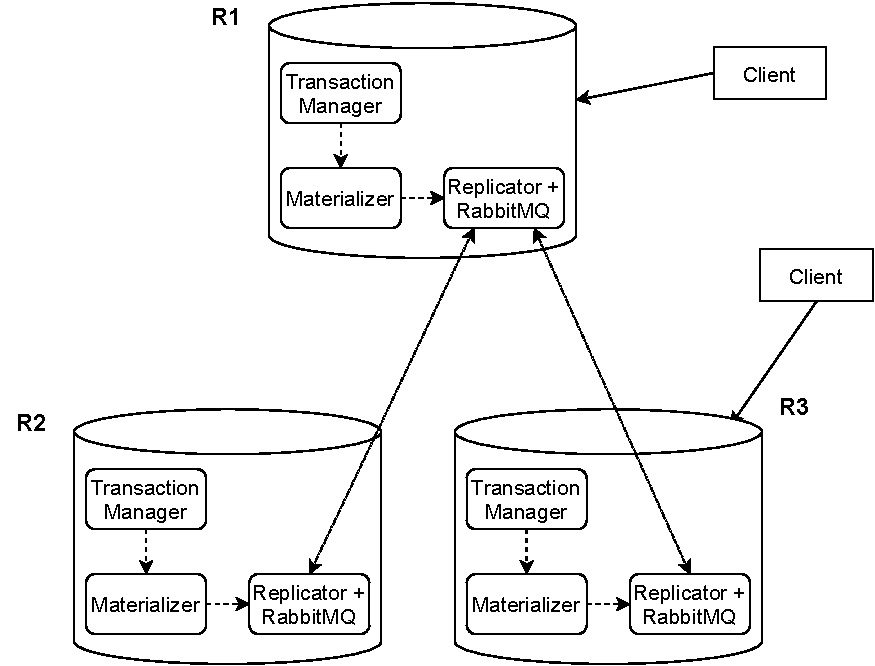
\includegraphics[width=.95\linewidth]{potiondb_architecture}
	\caption{PotionDB Architecture}
	\label{fig:potiondbArch}
\end{figure}

Figure \ref{fig:potiondbArch} illustrates PotionDB's architecture.
%PotionDB is a geo-replicated key-value store as illustrated in Figure \ref{fig:potiondbArch}.
Clients communicate with one or more servers to execute their operations.
Transactions are executed locally in one server, with updates being propagated asynchronously to other replicas.

Each replica contains only a subset of the objects - the system admin defines which groups (buckets) each server replicates (as described in Section \ref{subsec:dataAPI}).
If objects are partitioned correctly according to an application's needs, each client should only need to communicate with one server to do his operations, as all the data relevant to a client should be in one server.
In the case of not all required data being in one server, the client has two options:
\begin{enumerate*}[label=(\roman*)]
	\item contact other servers and execute a transaction on each server;
	\item send all the operations to one server, which will then request operations to other servers for objects not locally replicated.
\end{enumerate*}
%the client can either contact multiple servers and execute a transaction in each server.
Note that this case should be exceptional - in most cases views will be replicated in all servers, thus reducing the need to consult other servers.
We discuss this further in Section \ref{subsec:operationsNonLocal}.

\andre{Should I even mention Cure here, and if yes, what else should I say about it, mainly in terms of similarities/differences with PotionDB}

\andre{Maybe the figure reference should only be here?}

The internal architecture of each PotionDB replica is similar to Cure \cite{cure}.
Each PotionDB replica can be separated in three main components:
%\begin{enumerate*}[label=(\roman*)]
%\item TransactionManager (TM), which is responsible for receiving and replying to client requests, attributing timestamps to transactions and forwarding operations to Materializer;
%\item Materializer (MAT) which stores the object and applies both local and remote read/write operations, ensuring parallel snapshot isolation while executing those.
%\end{enumerate*}

\begin{itemize}
	\item TransactionManager (TM), which is responsible for receiving and replying to client requests, attributing timestamps to transactions and forwarding operations to Materializer;
	\item Materializer (MAT) which stores the object and applies both local and remote read/write operations, ensuring parallel snapshot isolation while executing those.
	Local updates of a transaction are forwarded to the replicator once the transaction finishes executing;
	\item Replicator + RabbitMQ is responsible for both propagating updates to other replicas as well as receiving them. Operations are replicated asynchronously. We give more details on the replication  mechanism in Section \ref{subsec:replication}.
\end{itemize}


%apresentar a arquitetura a nível geral.

%Explicar servidores, clientes, sincronização.

\section{Transactions over Partially Replicated Data}

In PotionDB objects are partially replicated across the servers.
Furthermore, views can refer to data not present in the local replica.
Both factors can make it difficult to reason about the consistency guarantees of PotionDB.

Thus in this section we define precisely the consistency model provided by PotionDB.
We also define formally what a view object is in PotionDB.

%artigo com valter 2018, secção 2
%Definir matematicamente a consistência e as views
%- Ver a base de dados como sendo um conjunto de objectos e um conjunto de views, sendo que as views são uma função dos objecto(s)
%- Definir como estão as views num dado snapshot
%- Ou seja, a consistência de ler... e manter up-to-date.

\subsection{Views}

We define a PotionDB database as a set of objects partially replicated across multiple servers.
Updates and reads can be applied on an object.
A transaction is a list of updates and/or reads for one or more objects.
Each object has a bucket associated, with all objects in a bucket being replicated in the same subset of replicas. %\emphfunction{B}{o} returns the bucket of an object \emph{o}.

We consider a view to be any object for which it is possible to describe its state as being a function of object(s).
Assuming that \emphfunction{S}{o} returns the state of the object \emph{o}, we can say that \emphfunction{S}{v} = \emphfunction{F}{o_1, o_2, ..., o_n}, where $v$ is a view, $o_1, o_2, ..., o_n$ the objects which $v$ is based on, and \emph{F} the function that converts those object's state into the view's state.

Our views are updated in the same transaction as the objects they refer to.
%That is, $\forall v : \exists u_o \in T \land S(v)=F(o, ...) : \exists u_v \in T$
That is, $\forall v: \exists u_o \in T \land S(v)=F(o, ...) : \exists u_v \in T$, where $u_o$ and $u_v$ represent updates for, respectively, object $o$ and view $v$ in transaction $T$.
Non-formally, we assume there is some mechanism that provides updates for all views which refer to some object being updated in a given transaction. %applying those view updates in the same transaction.
%We discuss the implications of partial replication on updating views in Section \ref{subsec:partialReplicationViews}.

\subsection{Consistency}

PotionDB supports both Parallel Snapshot Isolation (PSI) \cite{walter} and Read committed (RC) as its consistency models.
We now explain precisely which guarantees PotionDB provides under each model.

\subsubsection{Parallel Snapshot Isolation}

To start with, consider only one server and the Snapshot Isolation (SI) model. 
SI allows each transaction to access a consistent view (snapshot) of the database.
More precisely, a snapshot can be defined as the sequence of transactions that happened before said snapshot.
Assuming $SN_i$ represents the initial empty state of the database, a $T$ represents a transaction, we can define a snapshot $SN_n$ as the result of $T_m(T_{m-1}(...(T_1(SN_i))))$, where $T_1$ ... $T_m$ represent the list of transactions that happened-before $SN_n$.

All transactions issued in a replica can be serialized.
That is, given any local transactions $T_1$ and $T_2$, either $T_1 \prec T_2$ or $T_2 \prec T_1$.
When a transaction commits, its updates are executed according to the issued order.
Furthermore, for any two local transactions $T_1$ and $T_2$, if  $T_1 \prec T_2$, then $\forall u_n \in T_1 \land \forall u_m \in T_2 : u_n \prec u_m$.

It was previously stated that updates for a given object and all the views that refer to it happen in the same transaction.
Given said statement, along with our snapshot definition, the following theorem can be defined:

\begin{theorem}
	\label{theorem:viewobj}
	Given any object $o$ present in snapshot $SN_n$, the state of all views which refer to object $o$ matches the respective function $F$ that describes a view's state based on the object $o$.
\end{theorem}

Informally, Theorem \ref{theorem:viewobj} states that for any given object $o$ in snapshot $S_n$, all views that refer to it are consistent and thus include the effects of all operations applied to $o$ until snapshot $S_n$.

\andre{Anything else I need to define for snapshot isolation?}

Consider now multiple servers, as well as the model Parallel Snapshot Isolation (PSI).
PSI is an extension of SI, allowing for transactions executing in different servers to have different commit orders - that is, transactions can be concurrent if they commit in different servers.
This implies that transactions originated from different servers may have a different execution order from server to server.
Two transactions $T_1$ and $T_2$ are considered concurrent if $T_1 \not\prec  T_2 \land T_2 \not\prec  T_1$.

%A serialization of transactions under PSI is considered valid if the order of execution of the transactions respects the happens-before relationship. That is, for any $T_1 \prec T_2$, $T_1$ must be serialized before $T_2$.
%For concurrent transactions, any order which does not break the happens-before relationship with other transactions is valid.

A serialization of transactions under PSI is considered valid if the order of execution of the transactions respects the happens-before relationship.
To be precise, $\forall T_1, T_2 : T_1 \prec T_2 : T_1 \Rightarrow T_2$, where $\Rightarrow$ denotes that the left transaction is serialized before the right transaction.
Note how there is no restriction for concurrent transactions - as long as the happens-before relationship is respected, concurrent transactions can commit in any order, possibly in different orders in different servers.
In PotionDB, the usage of CRDTs ensures the states of different replicas will eventually converge even if concurrent transactions are applied in different orders.

\andre{Section \ref{subsec:partialReplicationViews} describes the implications of partial replication in keeping views up-to-date. Do I need to refer that section here?}

\subsubsection{Read committed}

Read committed (RC) is a consistency model which guarantees that only states resulting from committed transactions can be read.
This model is ``weaker'' (less guarantees) when compared to PSI.
However, PSI has considerable overhead on reads in PotionDB, for scenarios with a high update rate, due to the provisioning of the snapshots.
Thus, we provide the option to use RC for when high read throughput is a must under a high update rate scenario.

For now, consider a single object in the database.
Under RC, PotionDB ensures that consecutive reads of the object read either the same state or a more recent state.
That is, for two reads of object $o$, $R_1(o)$ and $R_2(o)$, if $R_1(o) \prec R_2(o)$, then the state returned by $R_2(o)$ is either more recent or the same as in $R_1(o)$.
Also, no reads of ongoing (uncommitted) transactions can ever be read.
In other words, under RC, single-object causality is still ensured.

Consider now multiple objects in the database.
Under RC, PotionDB does not guarantee that if two objects are read simultaneously, the returned states will be in the same snapshot.
Thus, under RC it is possible to read an object and a view associated to it and observe unconsistent states (e.g., the view may not reflect the last update visible on the object).
In other words, under RC cross-object causality is not guaranteed - PSI must be used to have this property.

To be precise, the following is possible under RC:
$\forall R_1(o_1), R_2(o_2) : R_1(o_1) \in T \land R_2(o_2) \in T \land o_1 \not= o_2 :$ the states returned by $R_1(o_1)$ and $R_2(o_2)$ may be from different snapshots.

\andre{Do I need/should I do the correspondent property to the one above in the PSI section?}



%
%To be precise, the form of RC provided by PotionDB can be described as follows.
%Only states resulting from committed transactions can be read.
%Furthermore, once a version A is read from an object, any future read will return either version A or a more recent version.
%However, reads to different objects in the same transaction can read different versions.
%As such, single-object causality is ensured but cross-object causality is not.
%
%The main advantage of RC is the ability to still provide a high read throughput even under scenarios with a high update ratio.
%However, when cross-object causality is desired (e.g., when reading an object referred by a view), PSI should be used.


\if 0	

\section{Transactions over Partially Replicated Data}

\andre{The formal definition of PotionDB is already in section 3...}

In PotionDB objects are partially replicated across the servers.
Moreover, views may refer to data not present in the local replica.
For simplicity, we name objects that are referred by views as ``base objects''.
Furthermore, clients can access and modify multiple objects in the same transaction.
Any object in PotionDB is a CRDT, which allows objects to converge even in the presence of concurrency.

In this section we detail the consistency guarantees provided by PotionDB.
We also describe how transactions refering objects not locally replicated proceed, as well as the guarantees in said scenario.

%In PotionDB data is partially replicated across the servers.
%Moreover, views may refer to data not present in the local replica.
%In this section we first clarify the guarantees clients have when accessing non-view objects in PotionDB, and afterwards extend it for views. 

\subsection{Consistency}

PotionDB supports both Parallel Snapshot Isolation (PSI) \cite{walter} and Read committed (RC) as its consistency models.
We now detail each of the models, starting by assuming that all objects referred in a transaction are replicated in the same server (which is the intended use case of PotionDB).
We will drop this assumption later on.

Snapshot Isolation (SI) ensures that each transaction reads a consistent view (snapshot) of the database - that is, all objects are read in the same version, without interference from ongoing transactions.
SI also ensures that transactions which write to the same object can not commit concurrently - either one must be aborted or the transactions need to occour sequentially.
PSI extends SI by allowing transactions on different servers to have different commit orders - that is, transactions can happen concurrently if happening in different servers. 
The usage of CRDTs to represent objects ensures the state converge even with concurrent transactions in different servers.
We note that causality is still preserved - if server A executed transaction T1 before T2, T1 will execute before T2 in every other server.

%By default, PotionDB provides Parallel Snapshot Isolation (PSI) \cite{walter} as its consistency model.
%Transactions can both read and update multiple objects in a single replica.
%With PSI, PotionDB guarantees that all objects are read at the same version and that all modified objects will have the same new version.
%Furthermore, other clients only observe the state of the objects either before the effects of the transaction, or after - that is,
%the new version of the objects can only be read once the transaction has finished commiting and being applied.

%PSI allows concurrent operations to happen in different replicas, and such is possible in PotionDB.
%CRDTs ensure the states of remote replicas converge.
%We also ensure causality when considering remote operations - once a client sees the effect of a remote operation, any later read will reflect the effects of said operation.

Providing PSI has considerable overheads due to the isolation guarantee \cite{walter} and provisioning of snapshots.
Thus, PotionDB can also operate in a quicker, but weaker, consistency model - Read committed (RC).

To be precise, the form of RC provided by PotionDB can be described as follows.
Only states resulting from committed transactions can be read.
Furthermore, once a version A is read from an object, any future read will return either version A or a more recent version.
However, reads to different objects in the same transaction can read different versions.
As such, single-object causality is ensured but cross-object causality is not.

The main advantage of RC is the ability to still provide a high read throughput even under scenarios with a high update ratio.
However, when cross-object causality is desired (e.g., when reading an object referred by a view), PSI should be used.

%Due to the isolation required to provide SI, PotionDB also provides the option of doing ``fast reads'' with less guarantees.
%Namely PotionDB provides the option for read committed.
%With this reads can be executed imediatelly and do not need to wait for any ongoing transaction to finish. 
%However, causality between objects is not ensured - a client may read object A in one version and then object B in a previous version.
%Single-object causality is still ensured though - if object A is read in version X, any further read done on object A by that client will be on version X or on a more recent version.

%\andre{Does this here need some justification on how this is acceptable for some use cases (and probably refer other DBs that do so? Also if we should refer that only with moderately high update rates are these fast reads needed.}

\subsection{Views}

Views can reflect data that is not present in the same replica as the view.
This poses questions in how views are kept updated and its relation with consistency.
We give details on the former in Section \ref{subsec:partialReplicationViews}, while focusing on the latter for this section.

Replicas of a view receive all updates for said view that occour in other replicas, even if a given replica does not replicate the base data that generated the view update.
Thus, views are kept up-to-date and complete in all replicas.
Views are also accessed as any other object, thus the consistency guarantees discussed in the previous section also apply to views.

It is important to note that under PSI, a client is able to read in a transaction both a view and its base data in the same version, assuming the base data is replicated in the server the client is accessing.
However, under RC, it is possible for different versions to be accessed in the same transaction when reading the view and its base data.


%One key challenge in PotionDB is keeping views synchronized with their base data, even when part of that data is not replicated locally.
%It is also important to provide useful guarantees to the clients accessing the view, in order to facilitate application developing.
%To better explain our guarantees, we define four scenarios, based on the read consistency used and whenever a view's base data is present or not:

%\begin{itemize}
%\item PSI and base data present: a view and its base data are updated in the same transaction.
%Since all of a transaction's updates are applied at one point in time from the client's view, a view always reflects the latest data and is consistent with the base data.
%If a client fetches a view and a base data object in the same transaction, it is guaranteed that the same version will be provided for both.
%\item PSI and base data not present: the view is kept updated as view updates from other replicas are received.
%It is possible that the base data in a remote replica may be in a more recent version than the view in the local replica.
%However, it is guaranteed that eventually the local replica will receive all view updates from other replicas with relevant base data.
%\item Read committed and base data present: it is possible to read different versions for object and view even if done in the same transaction.
%PSI should be used if it is desired to read both the view and base data consistently.
%Noteworthy, since single-object causality is ensured, reading just the view will always wield the same version or more recent versions than the prior read's.
%\item Read committed and base data not present: single-object causality is ensured. 
%The view will receive updates from other replicas and will, eventually, reflect the latest state.
%\end{itemize}

\fi

\subsection{Operations on objects not locally replicated}
\label{subsec:old_operationsNonLocal}

In an optimal scenario, clients only need to access data that is present in a nearby server.
Ideally, partial replication is done in such a way that data is distributed according to its relevance in the geographical area where each server is located in.
This is also the scenario for which PotionDB is optimized.
We do however recognize the need for queries that may involve global data (namely analytic/statistical queries), hence why we provide materialized views of data not replicated locally.

Nevertheless, in case a client sporadically needs to access an object not served by a view and not locally replicated, the client has two options:
\begin{enumerate*}[label=(\roman*)]
	\item \label{remote1}directly contact a replica of the said object; 
	\item \label{remote2}request the operation on the server the client was already accessing.
\end{enumerate*}

Option \ref{remote1} is the expected use case and the fastest to execute, as the request can be done concurrently while still operating on the original server.
Option \ref{remote2} is also provided, however, for ease of use and for when it is intended for the object to be accessed in the context of an already ongoing transaction.
We note, however, that option \ref{remote2} is slower - internally, what is done is that the server receiving the request redirects it to another server and awaits its reply.
That is, the transaction will be on hold until the other server replies and the client is, effectively, paying 2 round-trips of latency (between servers + server the client is contacting).
Finally, we note that in the current implementation of PotionDB, only RC is ensured for remote reads - a different version from the local objects may be returned by the remote read.

We believe for most use cases, good data locality when doing partial replication, alongside the usage of views, will make needing to access other replicas a very sporadic event.
We note that data which may be revelant everywhere can still be replicated in every server if desired.

%Garantias
% Snapshot isolation
% Read committed
%Modelo de Consistencia?
%Modelo de consistencia no acesso às views (garantias do utilizador)

\section{Supporting Views}
\label{sec:views}

\andre{I ended up not mentioning the challenges of supporting views, but let me know if I should fit those somehow}

In this section we elaborate on the mechanisms we use in PotionDB in order to support views.
Namely, we detail how views are updated when a relevant object gets updated, how partial replication affects views and how we keep the storage overhead of views reasonable.

%\andre{Possible topics for this?}
%\begin{itemize}
%	\item "Introduction?" (challenges? As in Section \ref{sec:views})
%	\item NuCRDTs
%	\item Triggers
%	\item View distribution and transactions (that is, explain how we require views to be in every replica that contains base data relevant to the view + view updates are bundled in the same transaction as the base object update. Definitely needs a better title.)
%\end{itemize}
%
%\andre{Also check Section \ref{sec:views}... maybe most of it is okay/re-usable?}

\subsection{Triggers}
\andre{Please check for repetition/overlap with section \ref{subsec:viewAPI}}

When an object is updated, all views to which that object may be relevant must be updated as well.
Another concern is how updates to an object are converted into view updates, specially when considering that any object supported by PotionDB can be used as a view.
We leverage on the usage of triggers to deal with both concerns.

The intuition behind triggers in databases is to automatically do an action when a read or update to given object(s) happen.
Similarly to some relational DBs \cite{???}, in PotionDB we use triggers to automatically generate updates to views when related objects are updated.
In Section \ref{subsec:viewAPI} we presented the interface for triggers. In this section we focus on how they are used.

\subsubsection{Storage}

\andre{We likely need to refer in the replication section how we replicate triggers? }

We store triggers in PotionDB as plain objects, i.e., not as CRDTs.
They do not need to be handled as CRDTs since:
\begin{enumerate*}[label=(\roman*)]
	\item each trigger is immutable (it can not be modified after being created);
	\item we assume trigger names are unique and, thus, there will not be any concurrent add/remove of a trigger.
\end{enumerate*}
While the latter point may seem questionable, we believe it is a fair assumption as triggers will not be created commonly by the clients, as they are usually defined by system admins and often before the database is populated.
Triggers are replicated as explained in Section \ref{???}.

\subsubsection{Matching}

As shown on Section \ref{subsec:viewAPI}, triggers can either be specific to one object or generic and thus concern multiple objects.
Single-target triggers are stored in a map indexed by the trigger's source object key, type and bucket, thus allowing direct access when an object is updated.
On the other hand, generic triggers are stored in a different map indexed by the source object type, as well as the operation type that fires the trigger (both elements can not be generic).
When an update happens, the entry which contains the triggers (if any) for the source object and operation type is fetched.
For each trigger in said entry, the regular expression of the key and bucket is tested with the key and bucket of the object being updated.
A view update is generated if both match.

\subsubsection{Update generation}

\andre{two questions: a) should the part of clients applying the triggers be in its own subsection; b) should I mention that in the future we intend for servers to apply the triggers?}

On startup, clients fetch the list of triggers from a replica.
When a client intends to update an object, the triggers are checked as described in the previous section.
For all triggers that match, view updates are generated.
Both the original object's and all generated view's updates are grouped in the same transaction, thus ensuring PotionDB will apply all of them with the same logical clock.

Recalling the API presented in Section \ref{subsec:viewAPI}, all triggers have a source object and a target viewV.
The source operation defines which object(s) and operation fires the trigger, as well as any variables, while the view part defines the operation to be generated and to which object.
Any variables used in the source can be used in view operation.
When an update happens, the variables are replaced with the actual values.

\andre{Should I just use a figure/table for this example instead of the paragraph below?}

To exemplify, consider a trigger with a source counter identified by the triple (counter[0-9]*, bucket1, COUNTER) and the operation inc(c).
Consider also a topk view identified by the triple (topk1, bucket1, TOPK) and the operation add(counter[0-9]*, c).
The update inc(5) to the object (counter12, bucket1, COUNTER) would generate the update add(counter12, 5) to the topk view.

\subsection{Partial replication implications on Views}
\label{subsec:partialReplicationViews}

As previously mentioned, view updates are grouped with the source object in the same transaction.
PotionDB ensures that in a replica, all the updates of a transaction become visible at one moment in time.
This implies that a client can not see a state in which an object has been updated in a replica but its views have not.

%However, this still leave the following questions open: %\emph{How does partial replication affect views? How
%\emph{How do we ensure all replicas of a view receive view updates, even if they do not replicate the base data?}
However, this still leaves questions related to how partial replication may affect view updating. Namely, on how it is ensured that views are kept up-to-date even if not all relevant objects to a view are replicated in one replica.

%\andre{For as long as the clients generate the view updates, we don't require for views to be replicated in every replica. Do I still mention this? This section makes a bit less sense with triggers on client side.}

%\andre{The only thing that makes sense for now is to explain how }

%When a client wants to execute a transaction, all the operations are sent to one replica.
%A replica ignores all operations concerning buckets it does not replicate. 
%Thus if a client wants to manipulate objects which are scattered across multiple servers, the client must contact multiple servers and send a transaction to enough servers in order to ensure each object to be updated is replicated in at least one of those servers.
%This limitation can pose a problem concerning view updating - if a server contains an object relevant to a view but said view is not replicated there, the view update would be discarded.

Partial replication poses concerns related to keeping views up to date.
As each replica only applies updates to objects it replicates, if a replica contains objects relevant to some view but not the view itself, the view updates would not be generated and applied.

%\andre{I should refer in future work/some other place that we plan to address this limitation (not supporting updates for objects not replicated locally)? Do we actually want to address it? If not, we should justify/defend it}.

One possible solution for this is to require every server to replicate views.
This can be easily achieved by having one or more buckets just for views and having all servers replicate those buckets.
With this, a server will never discard an update to a view.
Due to how replication works (see Section \ref{subsec:replication}), this also ensures that all servers will replicate view updates and thus have their views up-to-date.
We note that this requirement is not a limitation - in fact, given the expected use case of PotionDB, it would already be desired for views to be replicated everywhere in most cases.
Even so, the exact requirement to keep views up-to-date is ligther:
more precisely, it is required for a view to be replicated in every server in which there may be objects relevant to the view.
This lighter requirement might be useful for cases in which the view doesn't concern data from the whole globe but instead, e.g., from one given country.

%16/03/21:
%Para a secção "Supporting Views":
%- Explicar NuCRDTs
%- Explicar como se actualizam as vistas
%- Triggers
%- juntar operações
%- Se for apresentar as dificuldades/desafios, fazer algo curto.
%- Não explicar a consistência aqui.

\subsection{Non-uniform CRDTs}

Non-uniform CRDTs (NuCRDT) leverage on the non-uniform eventual consistency model introduced by Cabrita et. al. \cite{Cabrita17Nonuniform}.
The observation is that with non-uniform eventual consistency, it is only required that the observable state is eventually equivalent in all replicas, instead of the states themselves.
Two observable states are defined as equivalent iff, for each possible query, the result is equivalent when executed on either states.
This allows to save both storage space and communication overhead, as not all updates in a NuCRDT must be replicated to all replicas.
For example, in a TopK CRDT, where K = 100, the states are observable equivalent as long as the 100 entries in the top are equal between states.
Thus, an operation that adds an entry which would sit outside of the top 100 may not need to be replicated.

NuCRDTs are specially useful to serve as materialized views, as they allow to keep summaries of data easily while also being space-efficient.
E.g., recall the e-commerce scenario described in Section \ref{sec:overview} and consider a topK of ``top 100 consumers who spent the most''. 
Even if there's millions of customers globally, each replica does not need to keep data for all customers in order to correctly apply reads in the topK CRDT.
PotionDB fully supports the usage of NuCRDTs for both objects and views.

Supporting NuCRDTs has the following implications in PotionDB.
When an operation is applied to a NuCRDT, it is verified if the observable state has changed.
The operation is only replicated if the observable state changed.
Otherwise, the operation is stored locally if it may be relevant at some point later.
If it is known that it will never be relevant (e.g., adding an element outside of the top for a TopK without removals), no information is stored.

\andre{Note: in theory, for fault tolerance purposes, even operations that do not change the visible state should be replicated to a subset of the replicas. This is, however, not currently supported by PotionDB. Should we mention we plan to address this in future work?}

As mentioned, some operations may become relevant later on due to the execution of other operations.
For example, consider a Top-K with 100 elements on the top, with many other elements outside of the top.
If one element from the top is removed, another element will need to rise to the top.
Since not all operations are replicated, it may happen that by the execution of a \emph{remove}, an \emph{add} may now need to be replicated.
This kind of operations (in this example, the add) are only replicated when they become relevant to the observable state.
This is supported in PotionDB as follows.
When a transaction is applied, new operations generated by NuCRDTs (the add in the example) due to the appliance of NuCRDTs' operations in the transaction (the remove in the example) are gathered in a new transaction.
The new transaction is then replicated to other replicas as any other transaction, as described in Section \ref{subsec:replication}.
After the new transaction is applied, the observable states in every replica will be equivalent again.

\andre{In short, in topk, when an element is removed from the top, the replicas may diverge for a while.}

PotionDB supports max/min, average, TopK (with removal) and TopSum (with increments + decrements) as NuCRDTs.
The TopSum in particular is interesting, as the original design only supports increments \cite{Cabrita17Nonuniform}, thus we had to extend the design to support decrements.

A key difficulty in supporting TopSum is deciding when an operation may be relevant.
For example, consider two replicas, where the smallest element on top is 10.
If both replicas add 6 to element ``a'', then ``a'' must be added to the top.
Thus, the following heuristic is applied to decide when to replicate elements not in top.
Consider element ``a'' not in the top.
First, the difference between the smallest element on top and the value of ``a'' that is known in every replica is calculated.
Secondly, we divide the difference by the number of replicas - let the result be called \emph{margin}.
If the sum of non-propagated values for ``a'' is equal or higher than \emph{margin}, then said sum is propagated to every replica.
The intuition behind this heuristic is that, if all replicas were to add \emph{margin}, ``a'' would go to the top.
If any replica adds at least \emph{margin}, said add is replicated, potentially triggering the non-replicated adds for ``a'' stored in other replicas to also be replicated, as margin will decrease when adds get applied.
If all replicas add less than \emph{margin}, it is safe as the element would not go to the top even if replicated.

\andre{We apply the same heuristic as defined in \cite{Cabrita17Nonuniform}. Should I mention that?}

To support the heuristic described above, the TopSum implementation stores both non-propagated and propagated values.
As for subtractions, they are handled as follows.
If the subtraction is for an element in top, or for when the top is still not full, it gets replicated.
Otherwise it is not propagated, as a subtraction on its own will never make an element reach the top.
The entry for non-propagated values is updated however, in order for the subtraction to be considered if said element should ever reach the top.



%%%%%%%%Old text%%%%%%%%%%

%Non-uniform CRDTs \cite{Cabrita17Nonuniform} leverage on the fact that, for certain objects, not all of the object's data is necessary to answer queries.
%E.g., in a topK, only the K elements with highest value are required to answer a query.
%Thus, non-uniform CRDTs capitalize on this by only requiring those K elements to be replicated in every replica, which allows to reduce storage overhead.
%
%Cabrita et. al. introduce the concept of non-uniform eventual consistency. 
%The key difference between eventual consistency and non-uniform eventual consistency is that, instead of requiring for the states of each object to be eventually equivalent, it requires for the \emph{observable} stables to be eventually equivalent \cite{Cabrita17Nonuniform}.
%Two states are defined as observable equivalent iff, for each possible query, the result is equivalent when executed on either states.
%This allows to save both storage space and communication overhead, as not all updates in a non-uniform CRDT must be replicated to all replicas \cite{Cabrita17Nonuniform}.
%
%Non-uniform CRDTs are specially useful to serve as materialized views, as they allow to keep summaries of data easily while also being space-efficient.
%E.g., recall the e-commerce scenario described in Section \ref{sec:overview} and consider a topK of ``top 100 consumers who spent the most''. 
%Even if there's millions of customers globally, each replica does not need to keep data for all customers in order to correctly apply reads in the topK CRDT.
%
%PotionDB fully supports the usage of NuCRDTs for its objects.
%Thus, when an operation is applied on a NuCRDT object, the operation is only replicated to all replicas iff that operation changed the visible state.
%Some operations however may only have an effect later (e.g: in a topK, an element may rise to the top after another one gets removed) \cite{Cabrita17Nonuniform}.
%Operations in this category are only replicated from one replica to the others when it affects the visible state.
%
%\andre{Should I specify, *clearly*, that all replicas "together" need to keep the whole CRDT state? As in, if we concatenated the state of each replica, we would get the full state. I already hint this in the previous paragraph.}

\section{Internal Partitioning and Replication}

%In this section we discuss three important design decisions in PotionDB:
In this section we describe two important mechanisms in PotionDB: internal partitioning and replication.
The referred mechanisms are essential in efficiently supporting queries on global data, while maintaing reasonable update performance and space overhead.

\subsection{Partitions}

\andre{I've decided to, for now, use here the terms partition/sharding for, respectively, internal \& external partitioning. Maybe I should do the same in previous sections (namely Section 4)?}

In PotionDB objects are partitioned both internally in a server and externally between different servers.
Internally, we partition in order to efficiently utilize multicore CPUs, while externally we partition to reduce the amount of data stored and processed in each server, making usage of data locality.

External partitioning was discussed in Section \ref{subsec:dataAPI}.
Thus, we now focus on how we do internal partitioning in PotionDB.
%To simplicify, we refer to external and internal partitioning as, respectively, sharding and partitioning.
%We now explain how both mechanisms work in PotionDB.
%Both partitioning mechanisms work differently and have different goals, which we explain in this subsection.

%\subsubsection{Partitioning}

Inside a PotionDB instance, objects are split across multiple partitions.
%In a PotionDB instance, objects are split across multiple partitions.
Each partition has one thread associated to it, which allows requests in different partitions to potencially be processed in parallel. 
Each object is assigned to one partition automatically, based on a hash of the composition of the object's key, bucket and type.
%Inside a server objects are split across multiple partitions.
%Each object is assigned to one partition automatically.
%The partition to which an object is assigned to is determined by computing an hash based on the object's key, bucket and type.

The intuition behind partitioning objects in a server comes from the observation that, by having data grouped in multiple ``slots'' (i.e., partitions), if different clients access objects in different partitions, then both requests can be processed in parallel by a replica without any conflict.
And if both requests are read only, they can be processed in parallel even if some objects are present in both requests, as reads do not conflict \cite{???}.

At a first glance it may seem odd to partition based on a hash with the goal of improving performance.
However, this is justified by the expected use of PotionDB - simirlarly to relational databases, the most frequent and complicated queries are expected to have, for each one, a single view that answers them directly, thus requiring only a single operation.
Due to the nature of hashing, these views are likelly to be spread across multiple partitions.
This implies that multiple queries can be executed concurrently without conflicts even in the presence of concurrent updates that only affect unrelated objects.
Our practical evaluation shows that this partitioning improves PotionDB's performance quite considerably. \andre{Does it actually show that? Should we show that?}
%TODO: This very likelly will not be included in the Practical evaluation section. I may have to run some benchmarks and report the results here.

\andre{What's below is probably not needed. It's just a comparison with other alternatives}

%A possible alternative to internal partitioning and still make use of multi-core CPUs would be to use locks to control access to the same object, in order to prevent write conflicts \cite{???}.
Other possible solutions to make use of multi-core CPUs are possible, for instance:
\begin{enumerate}
	\item \label{item:old_locks} using locks to protect the same object from being concurrently modified \cite{???};
	\item \label{item:old_multiplePotion} running multiple PotionDB servers in the same computer.
\end{enumerate}

%In theory this can lead to a considerate performance improvement, as each replica can make use of their multi-core CPUs by having one thread per partition to process requests.
%Other possible solutions include: 
%\begin{enumerate*}[label=(\roman*)] 
%\item \label{item:locks} using locks to protect the same object from being concurrently modified \cite{???};
%\item \label{item:single} using only a single thread \cite{???}.
%\end{enumerate*}

Alternative \ref{item:locks} is difficult to implement, as it is required to find the right level of lock granularity and when should locks be obtained/released \cite{???}. 
Special care is needed to avoid deadlocking concurrent transactions. 
There's also concerns with both fairness and overhead of obtaining locks.
Our solution does not need to lock data, thus it avoids the overhead from using locks, is easier to implement and does not have deadlocks.

As for \ref{item:multiplePotion}, this would imply more replicas running in the system, which increases both replication and storage costs.
This would also imply concurrency conflicts even in the same computer.
Finally, while this can allow more clients to be processed in the same period of time, and is quite easy to implement, it does not improve the performance of each client, as each transaction must be done in a single replica (and thread) to avoid breaking consistency. \andre{Does this need to be explained? The idea here is that we would lose the "write follows reads/writes" property.}

%As for \ref{item:single}, the solution does not take any benefict from  the multiple cores of nowadays CPUs \cite{???}. In section \ref{???}, we show that this solution has worse performance than ours, specially with read-only transactions.

%\subsubsection{Sharding}
%
%\andre{This has a lot of overlap with Section \ref{subsec:databasemodel}}
%
%Since PotionDB is a partially replicated \cite{???} database, it is necessary to have a mechanism which allows to precisely define in which servers should an object be replicated in.
%
%We achieve this by requiring each object to be identified not only by its key, but also by a ``bucket''.
%Buckets define groups of objects that are replicated in the same group of replicas. In other words, two objects with the same bucket value will be replicated in the same set of replicas.
%For each replica, the system admin can define which buckets will be replicated in it.
%
%To exemplify, recall the commerce example presented in Section \ref{sec:example}.
%The customers can be partitioned based on their country's continent by taking the following steps: 
%
%\begin{enumerate}
%	\item Define one bucket per continent;
%	\item Configure the servers so that each replica replicates the bucket of its continent + another one for fault tolerance purposes;
%	\item When adding a customer to the database, specify the bucket correspondent to the customer's continent.
%\end{enumerate}
%
%%PotionDB's replication mechanism takes in consideration the bucket distribution among servers, ensuring only servers interested in a given bucket receive updates for that bucket.
%It's worth noting that clients must ensure they are communicating with a server which replicates the buckets they want to operate on, since each server only replicates a subset of the buckets and doesn't forward operations to other servers.

\subsection{Replication}
\label{subsec:replication}

\andre{Note: If we decide to keep this section, maybe I should add a scheme showing each server "subscribing" buckets and another with the operations being sent?}

%Explain the basic idea of replication (async, partial, etc). Also include NuCRDTs here.
Replication in PotionDB is asynchronous and partial.
Operations are executed locally, without needing to contact other replicas.
Periodically, new updates are propagated asynchronously to other replicas.
All objects in PotionDB are operation-based CRDTs, thus the information required to propagate an update consists in the operation type and its arguments.

PotionDB uses RabbitMQ \cite{???} for handling communication between replicas.
RabbitMQ is a message brooker which allows consumers to register the topics of messages in which they are interested.
We leverage on topics to ensure each replica only fetches the messages containing updates for objects in buckets they are replicating.

We use RabbitMQ as follows.
Each PotionDB server runs alongside it a RabbitMQ instance.
When a replica starts, it contacts other server's RabbitMQs and subscribes to all messages whose topics match the buckets it replicates.
When a replica wants to publish new updates, it splits those updates by buckets (while maintaining causality), ensuring each message only contains updates for one bucket and whose topic value is that bucket.
Those updates are then sent to the local RabbitMQ instance, which then forwards them to interested PotionDB instances.
A receiving replica then rebuilds the transactions, applying the transaction once every update (for the buckets it replicates) of a transaction is received.
Causality related transactions will be applied according to their original order.

We also use RabbitMQ to support the addition of new replicas without stopping the system.
However, such mechanism is outside of the scope of this paper and thus we don't describe it here.

%\subsubsection{NuCRDTs replication}
%\label{subsubsec:nureplication}
%
%Non-uniform CRDTs \cite{Cabrita17Nonuniform} leverage on the fact that, for certain objects, not all of the object's data is necessary to answer queries.
%E.g., in a topK CRDT that only maintains the K elements with highest value, only those K elements must be replicated in every replica.
%
%The key difference between eventual consistency and non-uniform eventual consistency is that, instead of requiring for the states of each object to be eventually equivalent, it requires for the \emph{observable} stables to be eventually equivalent \cite{Cabrita17Nonuniform}.
%Two states are defined as observable equivalent iff, for each possible query, the result is equivalent when executed on either states.
%This allows to save both storage space and communication overhead, as not all updates in a non-uniform CRDT must be replicated to all replicas \cite{Cabrita17Nonuniform}.
%
%Non-uniform CRDTs are specially useful for using as materialized views, as they allow to keep summaries of data easily while also being space-efficient.
%E.g., if we consider the scenario described in Section \ref{sec:example} and a topK of ``top 100 consumers who spent the most'', even if there's millions of customers globally, replicas don't need to keep data for all customers in order to correctly apply reads in the topK CRDT.
%%E.g., in the scenario described in Section \ref{subsubsec:APIView}, even if there's millions of customers globally, replicas don't need to keep data for all customers in order to correctly apply reads in the Top-K CRDT.
%
%\andre{What's above, technically, isn't 100\% true: all replicas together need to keep ALL entries of the top-k due to removes being supported. Thus, an entry for all customers in the system. However, no single replica needs to keep all entries.}
%
%PotionDB fully supports NuCRDTs.
%Thus, when an operation is applied on a NuCRDT, the operation is only replicated to all of that CRDT's replicas iff that operation changed the visible state.
%Some operations however may only have an effect later (e.g: in a topK, an element may rise to the top after another one gets removed) \cite{Cabrita17Nonuniform}.
%Operations in that category are only replicated to all replicas when it affects the visible state.
%
%\andre{Should I refer that those operations in the last category are/should (as they aren't as of now) be sent to a few replicas for fault-tolerance purposes?}

\if 0

\section{Views}
\label{sec:oldviews}

Views are useful as they make it easier to specify queries and, in the case of materialized views, it may improve their performance as well.
An essencial question in supporting materialized views in a database is on keeping them coeherent with the base data they refer to.
When an object is updated the views must also be updated, otherwise the database becomes inconsistent which may then lead to errors in applications \cite{???}.

Usually in relational databases, views are updated automatically by using triggers associated to the base data tables \cite{???}.
Due to data being fully replicated and strongly consistent, it is guaranteed that at all times the view reflects the latest correct state \cite{???}.

PotionDB also uses triggers to keep the views updated. However, as PotionDB is a weakly consistent, partially geo-replicated database, extra challenges are imposed for maintaining materialized views up-to-date, namelly:
\begin{enumerate}
	\item Association between views and their base data. 
	PotionDB is a key-value store, thus multiple objects that would usually belong to the same table in a relational database (e.g., customers) have different keys associated.
	\item Automatic inclusion of objects created after the view that represent entities of the same kind (e.g., new customers) but necessarely have different keys.
	\item Translation of updates in base data to views. 
	Unlike in relational databases in which all data can be seen as tables with multiple columns, here there are multiple types of objects which have different kinds of properties and operations.
	\item Keeping the views and base data synchronized at all time.
	I.e., from the perspective of a client, updates on base data should lead to the view being updated simultaneously.
	%This isn't a problem in relational databases as they will belong to the same table.
	\item Keeping views updated even if all necessary data for it isn't present locally due to partial replication.
\end{enumerate}

In this section we detail the inner workings of views and triggers, and show how we address the points referred above.
We start by explaining what we define as a view, how are triggers used and updates generated for the views.
We end with discussing how our replication mechanism ensures view updates are sent to every replica that replicates those, even if they don't replicate the relevant base data.

\subsection{View CRDTs and Triggers}

We define as a view CRDT any CRDT that is updated automatically based on updates to other existing CRDTs.
To define how views should be updated, we leverage on the concept of triggers.

A trigger defines how updates on an object (source) translate to updates on another object (view).
The API was already described in Section \ref{subsubsec:APIVew}, thus in this section we focus on how triggers work internally.

\paragraph{Storage}We store triggers in PotionDB as special objects.
They do not need to be stored as CRDTs, as:
\begin{enumerate*}[label=(\roman*)]
	\item each trigger is immutable (it can not be modified after being created);
	\item we assume trigger names are unique and, thus, there will not be any concurrent add/remove of a trigger.
\end{enumerate*}
While the latter point may seem questionable, we believe it is a fair assumption as triggers will not be created commonly by the clients, as they are usually defined by system admins and often before the database is populated.
Triggers are replicated as explained in Section \ref{subsubsec:rabbitmq}.

\andre{Maybe the claim above needs a citation? Suggestions?}

\andre{Note: The storage description above is how I expect to implement it in the near future. At the moment clients store the triggers, but the next step will be for the servers to store them (clients will then have to fetch them)}

\andre{I probably need a better title for the paragraph below. Suggestions?}

\paragraph{Clients apply triggers} When a client starts, the existing triggers are fetched from the database, and stored on the client.
Then, whenever a client requests an update, it checks its triggers in order to generate the appropriate updates for the views.

\paragraph{Matching} As explained in Section \ref{subsubsec:APIVew}, triggers can either be specific to one CRDT or generic (i.e., match with multiple source CRDTs).
Non-generic triggers are stored in a map whose key is the uid (key, bucket, type) of the source CRDT.
Thus, non-generic triggers can be directly indexed when an update to a source CRDT is issued.
On the other hand, for generic triggers, we index them by CRDT and operation type, as both the key and the bucket may be regular expressions.
For a given update, every trigger whose CRDT and operation type is equal to those of the update, is tested to see if the key and bucket respect the regular expressions and, thus, a view should be updated.

\paragraph{Update generation}
Each trigger contains both a source operation and a view operation, which are relative to, respectively, the source and view CRDTs.
On the source operation we can define variables that will then be used on the view operation. E.g., if the source operation is \emph{inc(c)}, the 'c' is a variable that can then be used in the view operation, e.g., \emph{add('id1', c)}.
When an operation is prepared, the variables are replaced by their respective values, e.g., \emph{inc(5)} gets translated into \emph{add('id1', c)}.
Updates generated by triggers are added to the same transaction of the initial update, thus ensuring both updates to views and base data become visible at the same time.

\subsection{Implications of partial replication  on views}

%We now explain how views in PotionDB don't require all of its base data to be present in the same server as the view. To demonstrate this, we will first assume one of the servers contains all the base data for a given view, and then drop such assumption.
We now explain what are the implications of partial replication in PotionDB's views and, more precisely, how does replication need to be configured in order for views to work properly.

For now, we will assume that there is one server (PotionDB1) which contains all the base data that may be used to generate a given view.
If the clients always contact PotionDB1 to update such base objects, and thus the view, PotionDB's replication mechanism would ensure that all replicas which replicate the view's bucket would receive its updates (see Section \ref{subsubsec:rabbitmq}).
Since updates are sent separately, grouped by bucket, other replicas will receive the view updates as long as they replicate the view's bucket, even if they don't replicate the respective base data.
Thus, we have concluded that it is not necessary for every replica to replicate the base data of a view, as long as one server has all the base data.

We now drop the assumption that one server has all the base data, assuming instead that all relevant data is split across multiple servers.
Assuming that when a client wants to update one of the base objects, the contacted server (PotionDB2) replicates such object, we have two scenarios:
\begin{enumerate*}[label=(\roman*)]
	\item PotionDB2 replicates the view and, thus, both updates to base data and view are applied and replicated to other replicas (as described previously);
	\item PotionDB2 doesn't replicate the view, thus updates to the view are ignored, as we require that clients send their updates to servers which replicate the referred buckets.
\end{enumerate*}
In short, whenever a base object is updated, as long as such server also replicates the view's bucket, both the base object update and view's will be replicated to the relevant servers.

With this, we can now define how replication must be configured in order for views to work correctly.
The simpler solution is to have a special bucket for views, which is replicated in every server.
This ensures some server will always have any data that may be relevant to the view.
However, the precise requirement is that a view's bucket must be replicated in every server that contains, or may eventually contain, objects relevant to such view.

We note that it would be possible to ease this requirement further if the clients send updates of base data and views to different servers, as in this case one single server replicating the view would be enough, even if such server had none of its base data.
However, this would imply that the update of the view and of the base data would not be in the same transaction.
This in turn has the downside of, in servers which replicate both the view and some of its base data, to have the updates of the view and base data applied at different times, thus possibly giving an inconsistent representation of the database to the client for a certain period of time.

%Explain how it isn't necessary to have all data replicated everywhere, and how it suffices to have views replicated in every replica in which there may be a relevant base data.
%

%Explain how triggers are stored and used
%Server stores them on a special object; clients fetch triggers; clients generate view updates
%Explain the update procedure on clients
%Prepare main update; check non-generic triggers; check generic triggers; send all updates
%Address points 4 and 5 - same transaction; bucket mechanism ensures view updates are sent to every replica.

\fi

\section{Designing views for applications}

\andre{This probably needs a better title}

In order to evaluate PotionDB's performance, as well as better grasp the expressivity of views in PotionDB, we implemented TPC-H's data model, along with the set of possible updates and a subset of the proposed queries.
In this section we discuss the experience of adapting a SQL-oriented database scenario (TPC-H) to PotionDB, namely focusing on how we designed the views and limitations of our solution.

\subsection{Dataset and partitioning}

TPC-H's \cite{tpch} data set represents an e-commerce scenario, similar to the one described in Section \ref{sec:overview}.
Tables are used to represent customers, suppliers, products (parts), orders, nations and regions (continents).
Two extra tables represent associations: ``partsupply'' and ``lineitem'' represent, respectively, a product which one supplier can sell and a product sold in an order.

The dataset is adequate for partial replication.
We created a bucket for each region, and partitioned each table as follows:

\begin{itemize}
	\item Customer, Supplier, Nation, Region, Orders, Partsupply: associated to one region bucket. 
	All but orders and partsupply have a nation or region directly associated to it, which is used to select the bucket.
	For orders and partsupply, we select, respectively, the customer's region and supplier's region.
	\item Parts: associated to the bucket ``parts'' which is replicated in every replica.
	This is due to the fact that multiple suppliers across the globe may supply the same part; customers across the world can also order the same part.
	\item Lineitem: associated to both the customer's and the supplier's region.
	The details of an ordered object may be relevant for the customer, as well as the supplier.
\end{itemize}

We highlight that views are replicated in every server (they have their own bucket).
Thus, queries that may access data from multiple regions (e.g., the percentage of revenue from sales in which the supplier is not in the same region as the customer) can still be served efficiently.
We also note that lineitems being associated to two regions is not as problematic as it might look at first glance.
As each server has one region associated to it (plus another one for fault-tolerance purposes), very few lineitems will be duplicated in the same server.
Updating and storage costs are still quite lower than if we fully replicated lineitems, as even with duplication, the amount of lineitems in each server is quite less than if fully replicated.

\andre{One detail which I did not mention, as I think it might be confusing at this point - if we have some view that may be triggered by some new/deleted/updated lineitem, we can deterministally choose, e.g., to only generate a view update for the bucket of the supplier's region. That is, duplicated view updates are not possible even with duplicated lineitems.}

\subsection{Converting tables to objects}

\andre{Note: I'd expect to many others having done this to test key-value DBs. Should I refer any of those? If so, any paper suggestions are welcome :)}

All the tables in the TPC-H scenario have either an unique key (e.g., customer key for customer) or multiple keys that, when combined, are unique (e.g., part key + supplier key for partsupply).
Thus, we use those as the keys for our objects.

Each entry in a table maps directly to a map CRDT. E.g., each customer has a map representing it, with the object's key being the customer key.
The fields of a table are also CRDTs - we use whichever data type most closely matches the data in the tables (e.g., registers for strings, counters for numbers, etc.).
Buckets are associated to each object as described in the previous section.

\subsection{Designing views for queries}

\andre{I don't think this introdutory text is good - I need some help here.}

\andre{I think having a scheme (image) to show the resulting view of a query, as well as how it is accessed, would be useful. I'll work on that later on.}

\andre{I selected to explain the query 18 (Q18). Here's my thoughts behind each query implemented in PotionDB: \\
	- Q3 is not complicated to explain, however the motivation query is too specific (not an interesting ``question'' to answer). \\
	- Q5 is easy to explain, has good motivation, but data is local to a region. \\
	- Q11 is somewhat tough to explain (complicated SQL query). Decent motivation query. Also the views for this don't need updates.\\
	- Q14 is too simple. It has a good motivation query however. \\
	- Q15 is okay to explain, has good motivation query, but it's the only query where TPC-H authors themselves define a view. \\
	- Q18 has a decent motivation query, is okay to explain. Uses topK too.
}

Given a query, designing the view(s) appropriate to answer said query consists in figuring out how can the type of CRDTs offered by PotionDB be combined to, ideally, reply to the query in a single read operation.
%The idea is to have the view configured in such a way that, by applying a defined list of steps, we can fetch the reply to the query with just one read operation.

To design views, we define the following guidelines to ease the process:

\begin{itemize}
	\item Filter the data by using maps, or different views. E.g., if all the variations of a query always ask for the data of a month, use a map with one entry per month, or a view for each month.
	\item Some SQL keywords have direct equivalents in CRDTs. E.g., avg() corresponds to the average CRDT, sum() to counter, limit() to topK, etc.
	\item Views can be composed of multiple objects, and ``normal'' objects can be used as views too.
	For example, a counter can be used as a view to answer a query like ``total number of orders done by a client''.
	Another example consists in using a map inside of another map to efficiently filter data with multiple parameters, e.g., by nation and year.
\end{itemize}

To illustrate the process of defining views, consider query 18 (Q18) of TPC-H \cite{tpch}. The SQL query is defined as follows:

\vspace{1em}

``Return the first 100 rows:''

\emph{select}

\hspace{1.5em} c\_name, c\_custkey, o\_orderkey, o\_orderdate, o\_totalprice, \\sum(l\_quantity)

\emph{from}

\hspace{1.5em} customer, orders, lineitem

\emph{where}

\hspace{1.5em} o\_orderkey in (

\hspace{3em} \emph{select}

\hspace{4.5em} l\_orderkey

\hspace{3em} \emph{from}

\hspace{4.5em} lineitem

\hspace{3em} \emph{group by}

\hspace{4.5em} l\_orderkey having sum(l\_quantity) $>$ \{argQuantity\}

\hspace{1.5em}) and c\_custkey = o\_custkey and o\_orderkey = l\_orderkey

\emph{group by}

\hspace{1.5em} c\_name, c\_custkey, o\_orderkey, o\_orderdate, o\_totalprice

\emph{order by}

\hspace{1.5em} o\_totalprice desc, o\_orderdate

\vspace{1em}

In short, this query tries to access the top 100 customers who have placed a large quantity order, using as a sorting criteria the total value of the order.
The minimum value for an order to be considered ``large'' is represented by \{argQuantity\} and is a parameter of the query.
In the where clause, there's an inner query, which in practice collects all orders whose total quantity of ordered items is higher than \{argQuantity\}.

As referred, the only argument of this query is \{argQuantity\}, which is defined in TPC-H as being an integer in the range [312, 315].
Since we're only interested in one quantity at a time, and they have a limited range, we can associate each quantity's data to a different view object.
This has two implications: first, a read of a given quantity only needs to read one of the objects; second: an update may need to update multiple view objects.
E.g., a new order with 314 ordered items implies updating the view for quantity 312 and 313.

The next step is decide which CRDT(s) each object should use.
The ``return the first 100 rows'', as well as the order by, suggest using a TopK CRDT to hold the view's data.
To be more precise, we use a TopK CRDT in which each pair has as ID the l\_orderkey (as suggested by the group by of the internal query) and as value the o\_totalprice.
In each pair we also append c\_name, c\_custkey and o\_orderdate as extra data.
This extra data is optional - the intention is that fetching it directly from the TopK is faster than fetching the customer's and order's data alongside the TopK, specially as that could require accessing more than one server.
This represents a trade-off between extra view data and query execution speed, which should be considered when designing views in PotionDB, similarly to in relational databases.

\andre{I don't really have any specific logic that I use as reference to define the updates... I just think on how to translate an object update into a view update.}

For the context of TPC-H, the dataset is static apart from orders and lineitems.
Orders (and their respective lineitems) can be added and removed, but each object is immutable.
Thus, to keep views up to date, we only need to consider the addiction/removal of orders and lineitems.

For the query considered (query 18), the trigger for deletion is rather simple:

\firstblockemph{\hspace{-1.2em}Create Trigger q18Removal}

\middleblockemph{\hspace{-1.2em}On (order*, bucket, MAP)}

\middleblockemph{\hspace{-1.2em}With MapDelete(orderkey)}

\middleblockemph{\hspace{-1.2em}Do (}

\middleblockemph{\hspace{-0.5em}	Update ("q18\_312", "views", TOPK) With remove(orderkey)}

\middleblockemph{\hspace{-0.5em}	Update ("q18\_313", "views", TOPK) With remove(orderkey)}

\middleblockemph{\hspace{-0.5em}	Update ("q18\_314", "views", TOPK) With remove(orderkey)}

\middleblockemph{\hspace{-0.5em}	Update ("q18\_315", "views", TOPK) With remove(orderkey)}

\lastblockemph{\hspace{-1.2em})}

Removing on the four views may seem unecessary, as not all orders have large enough quantities.
However, by the TopK CRDT definition, if an entry does not exist in the TopK, then a removal is a no-op.
In other words, if the order was not on the views, then the remove will have no effect and thus does not need to be propagated.

\andre{In relation to what's above, another possible solution would be to add an extra field to orders to know the amount of items ordered and thus know which TopKs to remove from. The current implementation of the clients keeps this information.}

The addition is more complex.
For a new order, it is necessary to add up the amount of the items in that order, to know if the order should be added to the views.
As such, it is necessary to define code that, when a new order is added, sums the quantities of the items being added with that order and, if they are above 312, fires the necessary updates.
The trigger (and a simplified pseudo-code) can be defined as follows:

\firstblockemph{\hspace{-1.5em}Create Trigger q18Add}

\middleblockemph{\hspace{-1.5em}On (order*, bucket, MAP)}

\middleblockemph{\hspace{-1.5em}With MapAdd(orderkey, custkey, orderdate, totalprice, ...)}


\middleblockemph{\hspace{-1.5em}Do Code} (

\hspace{2.5em}let sumAmount = 0

\hspace{2.5em}for lineitem in transaction \{

\hspace{3.5em}if (lineitem.orderkey = orderkey) \{

\hspace{4.5em}sumAmount += lineitem.amount

\hspace{3.5em}\}

\hspace{2.5em}\}

\hspace{2.5em}//Views are for 312-315. -1 to account for $>$ quantity

\hspace{2.5em}sumAmount = max(sumAmount-1, 315)

\hspace{2.5em}if sumAmount $>$= 312 \{

\hspace{3.5em}let custName = \emph{Get (custkey, bucket, MAP) With MapGetField("c\_name")}

\hspace{3.5em}for i = 312; i $<$= sumAmount; i++ \{

\hspace{4.5em}\emph{Update ("q18\_" + i, "views", TOPK)}

\hspace{4.5em}\emph{With add(orderkey, totalprice, custName, orderdate)}

\hspace{3.5em}\}

\hspace{2.5em}\}

\lastblockemph{\hspace{-1.5em}})

In short, whenever a new order is defined, the trigger looks into the lineitems defined in the transaction for said order.
It is important to note that for TPC-H, the items of an order are all defined alongside the order itself, so this search can be implemented by looking at the operations defined before the order, until a non-lineitem operation is found.
The amounts of the items of the order are summed up, and if the summed amount is at above 312, updates are fired for the respective views.

For other queries the same steps were done: analyse the query, decide on CRDT(s) to implement the view and then define triggers to generate updates to the object view(s).

\andre{Does this needs some concluding note?}

%The simplest (but not necessarely the most efficient) solution is to define two triggers per view, one for the addition and another for the removal.
%The only difference between triggers is the necessary quantity for the order.

%The trigger for a new order looks as follows:

%Create Trigger q18New312
%On (order*, bucket, Map)
%With MapUpdate(orderkey, orderdate, totalprice, (...))
%Do Update (q18\_312, views, TOPK)
%With add()

\subsection{Limitations}

The main limitation of PotionDB's views is that they are designed for recurring queries - that is, each view is defined to precisely answer a given query.
As such, for scenarios in which the set of queries is constantly changing, it might be challenging to define views and triggers in PotionDB to serve those queries efficiently.

Another shortcoming comes from the triggers themselves - for more complex queries, it may be necessary to define custom code for the trigger's body.
This can raise security and safety concerns.
We note however, that this is an implementation shortcoming and not a design one - it would be possible to use an existing data manipulation language (e.g., \cite{oracleTriggers}) instead of custom code.

\andre{Any suggestions for further limitations?}


\subsection{Discussion of implemented TPC-H queries}
\label{subsec:implementedQueries}

\andre{Note: This should be somewhere else (maybe its own section? Suggestions?), but for now I'll leave it here}
\andre{TODO: Explain/mention TopSum in relevant sections}

To test PotionDB, only a subset of the TPC-H queries were implemented.
Thus, we had to choose a subset which represented different kinds of queries, spanning multiple types of CRDTs and scenarios.
We also considered how interesting the business question associated to each query is when selecting those, however here we focus on their relevance in testing PotionDB:

\andre{I'm not sure I should keep the last phrase above.}

\begin{itemize}
	\item Query 3: this query is interesting as it tests a multitude of things - it requires presenting data from different kinds of objects (lineitems, orders); updating requires accessing yet another kind of object (customer); tests viability of having a view for each day in a given period; tests implementing order by and limit with TopK CRDT.
	\item Query 5: this query was choosen to represent queries local to a region, i.e., queries that could be served only with data locally replicated, not requiring global views.
	Also tests the usage of maps to implement group by and counters for sums.
	\item Query 11: this query also limits the number of results returned but, instead of being e.g. ``limit 100'', it instead only returns results above a certain value, with this value being dependent on each nation's data.
	This thus requires a different approach to querying a TopK CRDT, and to maintaining both the TopK and the reference value updated.
	\item Query 14: this query was selected to choose yet another type of CRDT for views (average), as well as different kinds of the same object affecting the view differently.
	To be precise, lineitems on ``sale'' (tested with a string comparison) affect the view differently from those not on sale.
	\item Query 15: the main interest behind this query consists in it requiring to update the same entry in a ``top'' object multiple times.
	Thus, this requires using the TopSum instead of TopK in order to handle both increments and decrements to each entry as orders are added or removed.
	\item Query 18: this query requires the TopK to maintain extra data in order to query efficiently - data from customers, orders and a sum of lineitems is required.
	Another point of interest is how the views of this query are expected to have few entries compared other queries, thus it tests a scenario where triggers may be fired often but without having any effect.
	%The main source of interest for this query, however, is how it is expected to have usually few results to return while having to maintain entries for all orders.
	%Thus, this tests the efficiency of non-uniform replication in keeping only the necessary data to answer the query replicated in every replica.
\end{itemize}

As a final note, we highlight that we analyzed all queries of TPC-H.
While only the aforementioned 6 were implemented, we designed a possible set of views using PotionDB's objects that would be able to reply to each query defined in TPC-H.
Thus it is possible to support the full set of TPC-H queries in PotionDB, thus reinforcing the expressiveness of PotionDB's object types.

\andre{Should I mention that maybe the triggers would need to be more expressive to support updating all of those views? Then again we're already allowing custom code on them...}

\fi
